\documentclass[a4paper]{article}
\usepackage{spconf}

% \usepackage[utf8]{inputenc}

% \usepackage{graphicx, url}
% \usepackage{amsmath, amsfonts, xfrac}
% \usepackage{mathtools}

\usepackage{multirow}

\usepackage[utf8]{inputenc}

\usepackage[mathcal]{euscript}
\usepackage{booktabs}

\usepackage{graphicx, url}

\usepackage[cmex10]{amsmath}
\usepackage{amsfonts, amssymb, amsthm}
\usepackage{mathptmx}

\usepackage{caption}
\captionsetup{
  font = {footnotesize,up,singlespacing},
  skip = 1ex
}
\usepackage{subcaption}
\usepackage{float}

\usepackage[nocompress]{cite}


\usepackage{tikz}
\usetikzlibrary{positioning}

\newcommand{\Real}{\mathbb{R}}
\newcommand{\Cplx}{\mathbb{C}}

\newcommand{\pr}{\mathbb{P}}
\newcommand{\ex}{\mathbb{E}}
\newcommand{\var}{\text{var}}
\newcommand{\Pcal}{\mathcal{P}}
\newcommand{\Dcal}{\mathcal{D}}
\newcommand{\Ncal}{\mathcal{N}}
\newcommand{\Lcal}{\mathcal{L}}

\newcommand{\defn}{\mathop{\overset{\Delta}{=}}\nolimits}
\newcommand{\lpto}{\mathop{\overset{L^p}{\to}}\nolimits}

\newcommand{\re}{\operatorname{Re}\nolimits}
\newcommand{\im}{\operatorname{Im}\nolimits}

\title{Numerical study of the Crossing Tree for Self-similar Processes}
\twoauthors
  {Geoffrey Decrouez\sthanks{Thanks to the Centre for Advanced Studies for funding.}}
    {National Research University\\
    Higher School of Economics\\
    Moscow, Russia}
  {Ivan Nazarov}
    {IITP RAS\\
     Moscow, Russia}

\begin{document}
\maketitle

\begin{abstract}
The Crossing Tree is a recent tool, created to study scale invariance properties
exhibited by network traffic, financial time-series, and natural phenomena in physics
and biology, such as turbulence, earthquakes and heart beat. It provides an ad-hoc
representation of the data across a wide range of resolutions and independent of
its time scale. In this paper the theoretical and practical construction of the Crossing
Tree is presented. This tool is applied to analyse self-similar signals of processes
known as Hurst self-similar processes with stationary increments to gather evidence 
of the common features of the constructed crossing trees in this class of processes.
\end{abstract}


\section{Introduction} % (fold)
\label{sec:introduction}

Scale-invariance and self-similarity has been widely used lately to analyse a wide
range of time series, from medicine, to seismology, and to financial data. Essentially,
scale-invariance of some process implies that its dynamics is not characterized
by well defined dominant time-scales. Instead their dynamics involve all time-scales.
Analysing this kind of data should rely on identifying the mechanism relating the
scales with one another. The crossing tree (sec.~\ref{sec:the_crossing_tree}) is
a natural tool for analysing data at all scales simultaneously.

The structure of this paper is as follows. Sec.~\ref{sec:the_crossing_tree} outlines
theoretical and practical construction of a crossing tree, sec.~\ref{sec:h_sssi_processes}
reviews self-similar processes with stationary increments, which are used in the
Monte-Carlo study outlined in sec.~\ref{sec:experiment_setup}. Sec.~\ref{sec:results}
discusses the results of the numerical study and attempts to verify if the crossing
trees of $H$-sssi processes share common statistical properties. We conclude the paper
in sec.~\ref{sec:conlusion_and_further_work}.

% section introduction (end)

\section{The crossing tree} % (fold)
\label{sec:the_crossing_tree}

The crossing tree as a tool for analysing self-similarity goes back to the study
of diffusion on fractal sets (see ~\cite{BarlowPerkins88}). It was reintroduced
by in \cite{jones2004} in the context of studying self-similarity and regularity
patterns in network traffic data, where it has been proven to be successful in
detecting structural changes, manifested in changes in local regularity of the
time series. In this section I describe theoretical construction of the crossing
tree and how it is recovered from the discrete time series data.

\subsection{Crossing Times} % (fold)
\label{sub:crossing_times}

Consider a path of real-valued continuous process $\{X(t)\}$ with time running through
$[0,+\infty)$. Continuity is understood in the sense of the path of the process
being almost surely continuous, i.e. the set of discontinuous paths of $\{X(t)\}$
is a subset of a set of probability zero. At the heart of the crossing tree lie
crossing times of a uniformly spaced grid on $\Real$ given by $X(0) + 2^n\delta \mathbb{Z}$
for some $n\geq 0$ and base grid spacing $\delta > 0$.\footnotemark Each $n\geq 0$
represents the ``resolution'' through which sample paths of $\{X(t)\}$ are studied.
\footnotetext{The addition $x_0+A$, for $A$ in an affine space such as $\Real$
represents shifting of every element of the set $A$ by a common value $x_0$.}

The crossing times $T_k^n$ of process $\{X(t)\}$ at resolution $n\geq 0$ are defined
as follows: let $T_0^n = 0$ and for any $k\geq 0$ put
\begin{equation} \label{eq:xing_time}
  T_{k+1}^n = \inf \bigl\{
    t \geq T^n_k \,:\, |X(t) - X(T^n_k)| \geq 2^n\delta
    \bigr\} \,,
\end{equation}
-- the first passage time of a path of $X(t)$ across a level of $2^n\delta \mathbb{Z}$
different from the previousle crossed one. Fixing the zero-th crossing at $0$ aligns
the grid with the process. Therefore, without the loss of generality, we can consider
processes starting at the origin $X(0)=0$.

The crossing times of some fixed level $n\geq 0$ are non-decreasing by definition.
To show that $T_k^n < T_{k+1}^n$ we proceed by contradiction. Indeed, by right-continuity
of paths of $\{X(t)\}$ for $\delta 2^{n-1}$ there is $\eta>0$ with $|X(s)-X(T_k^n)| < \delta 2^{n-1}$
for all $s\in [T_k^n, T_k^n + \eta)$. But by definition of $T_{k+1}^n$ in the $\eta$
vicinity of $T_{k+1}^n$ there is $\hat{s}$ such that $|X(\hat{s})-X(T_k^n)|\geq 2^n\delta$.
Therefore, if $T_k^n = T_{k+1}^n$, then $2^n\delta \leq \delta 2^{n-1}$, which is
a contradiction.

Another property is that $|X(T_{k+1}^n) - X(T_k^n)| = 2^n\delta$ when $T_{k+1}^n$
is finite. Indeed, the function $t \mapsto |X(t) - X(T_k^n)|$ is continuous at least
at $T_{k+1}^n$, whence $|X(T_{k+1}^n) - X(T_k^n)| \geq 2^n\delta$. We proceed by
contradiction: if $|X(T_{k+1}^n) - X(T_k^n)| > 2^n\delta$ then by continuity there
is $s\in [T_k^n, T_{k+1}^n)$ with $|X(s) - X(T_k^n)| > 2^n\delta$, which would
imply that $T_{k+1}^n$ is not the greatest lower bound on all $s\geq T_k^n$ with
$|X(s)-X(T_k^n)| \geq 2^n\delta$.

% The crossing times of an almost surely continuous process $\{X(t)\}$ are such, that
% $T_k^n < T_{k+1}^n$ and $|X(T_{k+1}^n)-X(T_k^n)| = 2^n\delta$ for all $k\geq0$ with
% $T_{k+1}^n<+\infty$ almost surely.

The crossings of a continuous process have a natural tree structure when the times
are considered at different power-of-two resolutions of the grid $\delta \mathbb{Z}$.
To see this suppose that for some $k, m\geq 0$ we have $X(T_m^{n+1}) = X(T_k^n)$
and $T_k^n \in [T_m^{n+1}, T_{m+1}^{n+1})$. The definition of $T_{k+1}^n$ implies
that for all $s \in [T_k^n, T_{k+1}^n)$ we have
\begin{equation}\label{eq:xing_resol}
    |X(s) - X(T_m^{n+1})| = |X(s) - X(T_k^n)| < 2^n\delta \,,
\end{equation}
which implies $s \leq T_{m+1}^{n+1}$, since $T_{m+1}^{n+1}$ is the greatest lower bound.
Therefore $T_{k+1}^n\leq T_{m+1}^{n+1}$.

If the $(n+1)$-st crossing at resolution $m+1$ takes place, i.e. $T_{m+1}^{n+1} < +\infty$,
we get $T_{k+1}^n \neq T_{m+1}^{n+1}$. Indeed, if this were otherwise, $X(T_m^{n+1}) = X(T_k^n)$
and the continuity of sample paths would yield this contradiction:
\begin{equation*} \label{eq:contrad_1}
    2^n\delta = |X(T_{k+1}^n) - X(T_k^n)|
    = |X(T_{m+1}^{n+1}) - X(T_m^{n+1})| = 2^{n+1} \delta\,.
\end{equation*}

This assumption also implies that $T_{k+2}^n \leq T_{m+1}^{n+1}$. We proceed by
contradiction: having $T_{m+1}^{n+1} < T_{k+2}^n$ would imply
\begin{equation*} \label{eq:contrad_2}
    |X(T_{m+1}^{n+1}) - X(T_{k+1}^n)| < 2^n\delta \,,
\end{equation*}
where we used $T_{k+1}^n \leq T_{m+1}^{n+1}$ and the definition of $T_{k+2}^n$.
Finiteness of $T_{m+1}^{n+1}$ implies $|X(T_{k+1}^n) - X(T_k^n)| = 2^n \delta$
and $|X(T_{m+1}^{n+1}) - X(T_m^{n+1})| = 2^{n+1} \delta$. This, the triangle inequality
and $X(T_m^{n+1}) = X(T_k^n)$ imply
\begin{align*} \label{eq:xing_triang}
  |X(T_{m+1}^{n+1}) - X(T_m^{n+1})|
  &\leq |X(T_{m+1}^{n+1}) - X(T_{k+1}^n)| \\
    & + |X(T_{k+1}^n) - X(T_k^n)| \,,
\end{align*}
which leads to the following contradiction:
\begin{equation*} \label{eq:contrad_3}
  2^{n+1} \delta
    \leq |X(T_{m+1}^{n+1}) - X(T_{k+1}^n)| + 2^n\delta
    < 2^{n+1} \delta \,.
\end{equation*}

%% A nice picture is due here!!!!

% subsection crossing_times (end)

\subsection{Sub-crossing structure} % (fold)
\label{sub:subxing_structure}

Let's define the \emph{$n$-th level crossing} as the slice of the path of the process
over the half-interval $[T_k^n, T_{k+1}^n)$, $k\geq 0$, during which it moves exactly
$\pm 2^n\delta$. The properties of crossing times (sec.~\ref{sub:crossing_times})
imply that if $X(T_m^{n+1}) = X(T_k^n)$, $T_{m+1}^{n+1} < +\infty$, and
$T_k^n \in [T_m^{n+1}, T_{m+1}^{n+1})$ then
\begin{equation} \label{eq:duration_partition}
    \bigl[T_k^n, T_{k+1}^n\bigr) \cup \bigl[T_{k+1}^n, T_{k+2}^n\bigr)
        \subseteq \bigl[T_m^{n+1}, T_{m+1}^{n+1}\bigr)
    \,.
\end{equation}
The condition $X(T_m^{n+1}) = X(T_k^n)$ aligns different resolutions of the grid,
and $T_{m+1}^{n+1}<+\infty$ requires that the $(m+1)$-st crossing of the grid with
$(n+1)$-st resolution indeed took place.

%% Draw a simple illustration of the movements within one crossing
\begin{figure}
    \centering
    \resizebox{\linewidth}{!}{
        \tikzset{bullet/.style={circle,draw, fill=black,minimum size=5pt,inner sep=0pt},}
        \begin{tikzpicture}[grow=right, sloped]
    %% Crossings
            \node [bullet] (o) {};
            \node [bullet] (u) [above right = 3em and 9em of o.west, anchor = west] {};
            \node [bullet] (d) [below right = 3em and 9em of o.west, anchor = west] {};
            \node [bullet] (uu) [above right = 3em and 9em of u.west, anchor = west] {};
            \node [bullet] (ud) [above right = 3em and 9em of d.west, anchor = west] {};
            \node [bullet] (dd) [below right = 3em and 9em of d.west, anchor = west] {};
    %% The anchor and labels
            \node [draw=none] [left = 1em of o.west, anchor = east] {$X(T_k^n)$};
            \node [draw=none] [right = 1em of ud.east, anchor = west] {$X(T_k^n)=X(T_{k+2}^n)$};
            \node [draw=none] [right = 1em of uu.east, anchor = west] {$X(T_k^n)+2^{n+1} \delta$};
            \node [draw=none] [right = 1em of dd.east, anchor = west] {$X(T_k^n)-2^{n+1} \delta$};
    %% Crossing times nodes at the bottom
            \node [draw=none] (t2) [below =of dd.south, anchor = west] {$T_{k+2}^n$};
            \node [draw=none] (t1) [left = 9em of t2.west, anchor = west] {$T_{k+1}^n$};
            \node [draw=none] (t0) [left = 9em of t1.west, anchor = west] {$T_k^n$};
    %% Dumy nodes on the top level
            \node [fill=none,draw=none] (dummy2) [above = 1em of uu.north, anchor = north] {};
            \node [fill=none,draw=none] (dummy1) [left = 9em of dummy2.west, anchor = west] {};
            \node [fill=none,draw=none] (dummy0) [left = 9em of dummy1.west, anchor = west] {};
    %% Paths to levels
            \path[thick,draw]
                (o) edge node[above] {$+2^n\delta$} (u)
                (o) edge node[below] {$-2^n\delta$} (d)
                (u) edge node[above] {$+2^n\delta$} (uu)
                (u) edge node[below] {$-2^n\delta$} (ud)
                (d) edge node[above] {$+2^n\delta$} (ud)
                (d) edge node[below] {$-2^n\delta$} (dd);
    %% Crossing times
            \draw[black, dashed] (dummy2.west -| t2.west) -- (t2.west -| t2.west) {};
            \draw[black, dashed] (dummy1.west -| t1.west) -- (t1.west -| t1.west) {};
            \draw[black, dashed] (dummy0.west -| t0.west) -- (t0.west -| t0.west) {};
        \end{tikzpicture}
    }
    %% A very informative caption
    \caption{Possible movements over the $\bigl[T_k^n, T_{k+2}^n\bigr]$ interval.}
    \label{fig:xing_tree_structure}
\end{figure}

This implies that within the $(n+1)$-st level crossing there must be an even number
of subcrossings of the $n$-th resolution grid. Indeed, if $T_k^n = T_m^{n+1}$ and
$T_{m+1}^{n+1}<+\infty$, then there are two possibilities at $T_{k+2}^n$ (fig.~\ref{fig:xing_tree_structure}):
\begin{enumerate}
	\item the path returned to $X(T_k^n)$ level, in which case $X(T_{k+2}^n) = X(T_m^{n+1})$
    and thus by the time $T_{k+2}^n$ no crossing of $(n+1)$-st resolution grid occurred;
    \item at $T_{k+2}^n$ the path moved to a level other than $X(T_k^n)$, thereby
    inducing a crossing of $2^{n+1} \delta$ resolution grid.
\end{enumerate}
In the latter case $T_{m+1}^{n+1} \leq T_{k+2}^n$, and there are exactly \emph{two}
subcrossings, while in the former case the ordering of crossing times entails
\begin{equation*}\label{eq:subxing_order}
  T_{k+2}^n < T_{k+3}^n < T_{k+4}^n \leq T_{m+1}^{n+1} \,.
\end{equation*}
Since $T_{m+1}^{n+1}$ is finite iterative application of this argument implies that
there are even number of $n$-th level subcrossings during an $(n+1)$-st level
crossing.

Thus the properties of crossing times of a continuous process permit a natural tree
structure of crossings. If tree levels are enumerated from bottom up then
\begin{itemize}
	\item a node at the $(n+1)$-st tree level represents a crossing of the $2^{n+1} \delta \mathbb{Z}$;
	\item $n$-th level children (offspring) of an $(n+1)$-st level node represent the
	multiple crossings of a finer gird $2^n\delta \mathbb{Z}$ that took place during
	the larger crossing. 
\end{itemize}

The crossing tree reveals patterns of subcrossings within a parent crossing,
conditional on the direction of the latter. Denote the crossing orientations by
\[ \alpha_k^n = \text{sign}\bigl( X(T_{k+1}^n) - X(T_k^n)\bigr)
    \,. \]
Then subcrossing orientations of a complete crossing come in pairs by construction
of the crossing tree itself. Pairs of oppositely oriented crossings are
\emph{excursions}, and sign pairs ``$-+$'' and ``$+-$'' correspond to down-up
and up-down excursions, respectively, whereas pairs ``$--$'' or ``$++$'' constitute
direct upward and downward crossings, respectively. Any complete parent crossing
can be broken down into a series of excursions followed by a direct crossing, which
concludes the parent crossing by travsersing the next $\pm2^{n+1} \delta$ grid line.
Let $V_k^n$ be $0$ if the $k$-th $n$-level excursion (movements within a finer $(n-1)$-st
gird) is up-down: if $\alpha_{2k}^{n-1} = +$ and $\alpha_{2k+1}^{n-1} = -$, --
and $1$ if it is down-up (``$-+$'').

The above exposition considered the crossing tree for successively coarser resolutions
$2^n\delta \mathbb{Z}$ for $n\geq0$. For example in~\cite{decrouez2013estimation}
the crossing tree is defined for crossing times on this grid for any $n\in\mathbb{Z}$.
The restriction to non-negative levels in this paper was motivated by the fact,
that in practice, on real sample path of some supposedly continuous process it
is never possible no meaningfully go beyond some basic finest resolution given
by $\delta>0$. This has to do with the fact that processes are sampled at finite
frequency or over regularly spaced but finitely many points in time. However, it
is important to note that the crossing tree for resolutions finer than the base
scale give a one-to-one characterisation of the original continuous random process
in terms of the base scale, and crossing times $(T_k^n)_{k\geq 0}$ and crossing
orientations $(\alpha_k^n)_{k\geq 0}$, $n\in \mathbb{Z}$, \cite{decrouez2013estimation, ECP1673}.

% subsection tree_structure (end)

\subsection{Crossing tree on time series data} % (fold)
\label{sub:crossing_tree_on_time_series_data}

Here we briefly describe how the crossing tree is constructed for a sample
path of some continuous process, given by time series data $(t_i, x_i)_{i=0}^N$.

In practice the crossing tree is built iteratively from the finest resolution
specified by the base grid spacing $\delta > 0$. The crossing times of the leaves
of the tree are computed for a fixed and given $\delta>0$ in two passes: the first
pass computes passage times on the passed $x_0+\delta \mathbb{Z}$ grid levels, and
the second pass adjusts the passage times and passed levels to eliminate re-crossings
of the same level (recrossing events). The assumption that the time series data
came from a continuous process is the main reason, that enables a sequential procedure
for estimation of the crossing times of grid $\delta\mathbb{Z}$: recall, that
$X(T_{k+1})^n = X(T_k^n) \pm\delta2^n$ if $T_{k+1}^n<\infty$.

\begin{figure}[ht]
    \centering
    \begin{subfigure}{\linewidth}
        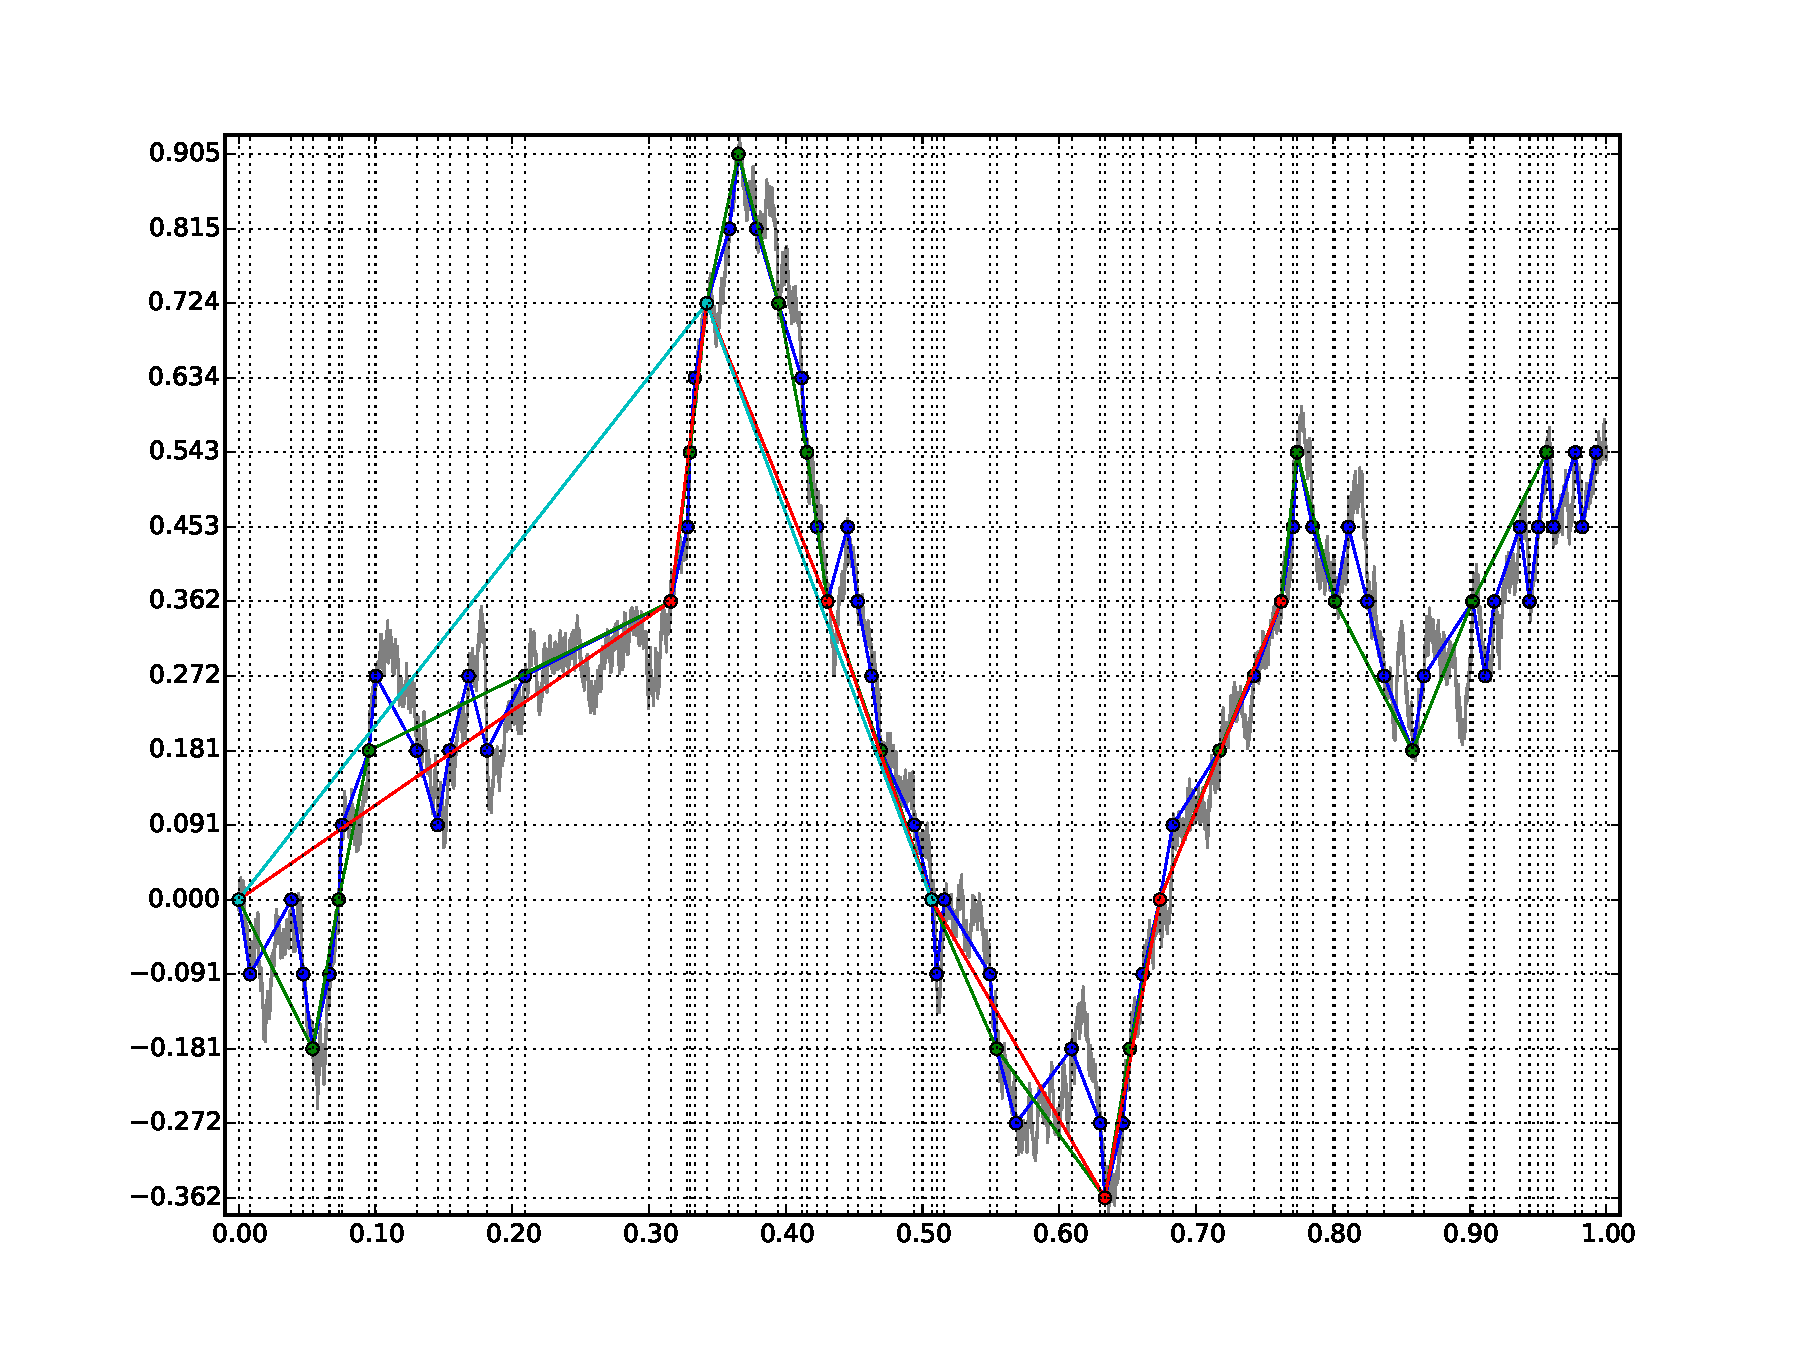
\includegraphics[width=\linewidth]{../plots/sample_path.pdf}
    \end{subfigure}\\
    \vspace{-20pt}
    \begin{subfigure}{\linewidth}
        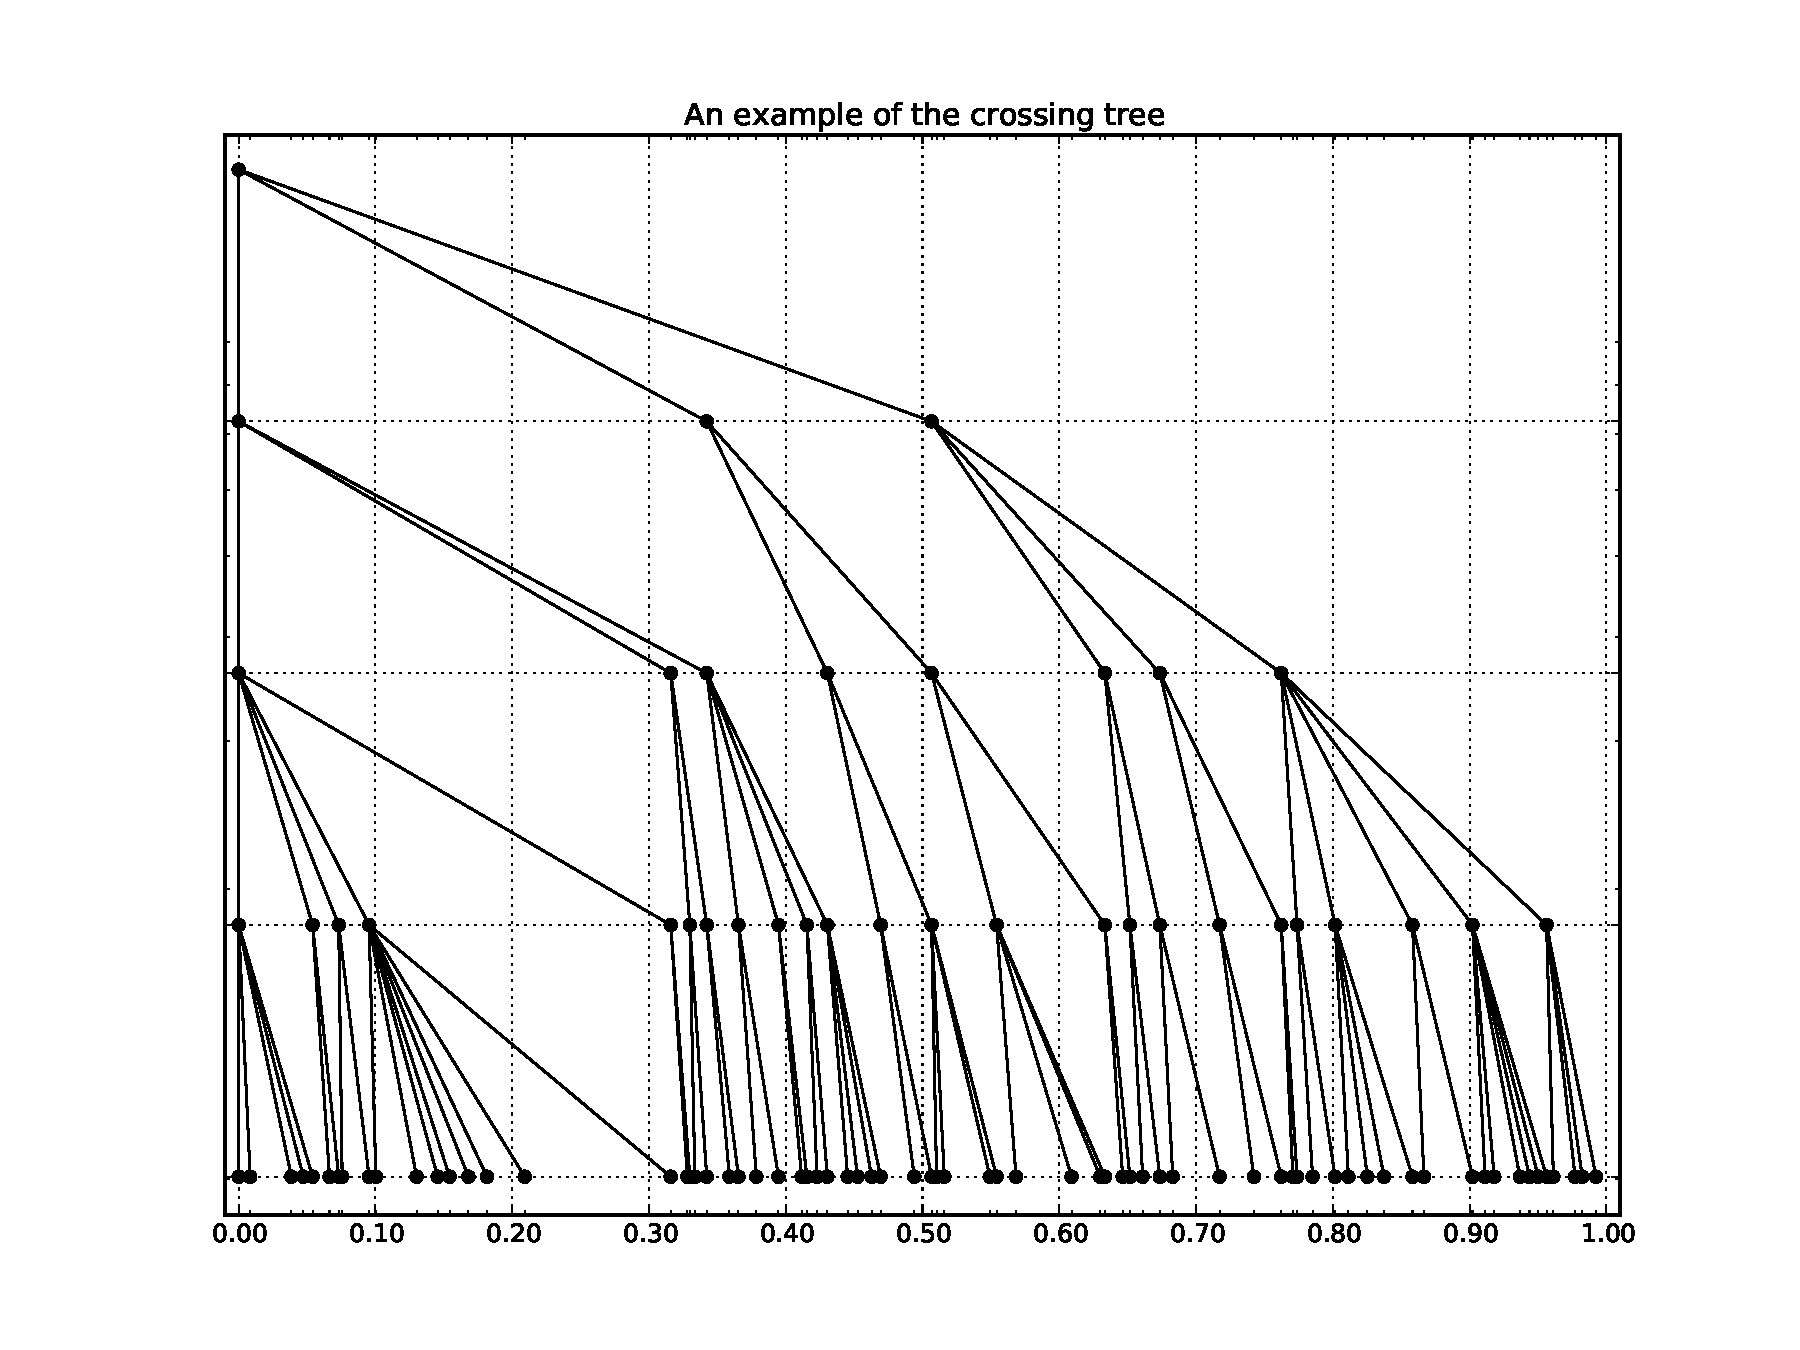
\includegraphics[width=\linewidth]{../plots/sample_tree.pdf}
    \end{subfigure}
    \vspace{-10pt}
    \caption{\emph{top}: the crossing times and levels of a sample trajectory of
    a continuous process; \emph{bottom}: the corresponding tree structure of the
    crossing times.}
    \label{fig:sample_tree}
\end{figure}

Once a crossing tree has been constructed for a particular sample path of a continuous
process $\{X(t)\}$ for a given base resolution $\delta>0$, it can be used to gauge
scale-invariance of the given realisation. Recall that the nodes of level $n$ of
the tree are crossings on the grid $2^n\delta$, and the offspring of each level
$n+1$ node correspond to the subcrossings of a finer grid $2^n\delta$ that constitute
the parent crossings. Typical crossing times and levels, and the corresponding crossing
tree is depicted on fig.~\ref{fig:sample_tree}.

% We briefly describe of the procedure for constructing the crossing tree on time series
% data $(t_i, x_i)_{i=0}^N$.

Recall that the tree is constructed in two passes: initial detection passages over
levels of $\delta \mathbb{Z}$ grid, which also discards within-band movements, and
the pruning phase, where re-crossing events are eliminated.

Before the first pass through the data, the time series $(x_i)$ is shifted and scaled
to series $z_i = \frac{1}{ \delta }\bigl(x_i - x_0\bigr)$, so that the constructed
tree is rooted at the crossing time $t=0$, since the process sets off from the origin.

The first pass sweeps through consecutive increments of the series given by pairs
$(t_i, z_i)$ and $(t_{i+1}, z_{i+1})$ for $i=1, \ldots, N-1$. For each increment,
its direction is determined by the sign of the difference $\Delta_i=z_{i+1}-z_i$,
and, depending on it, the range of grid levels traversed by it is computed. The
range of the $i$-th increment a subset of integers $R_i = [a_i,b_i]\cup\mathbb{Z}$,
where the boundaries $a_i$ and $b_i$ are determined using the following logic:
\begin{description}
    \item[Upcrossing] if $\Delta_i > 0$ then $a_i = \lceil z_i \rceil$
    and $b_i = \lfloor z_{i+1}\rfloor$;
    \item[Downcrossing] for $\Delta_i < 0$ the range given by $b_i = \lceil z_{i+1} \rceil$
    and $a_i = \lfloor z_i\rfloor$.
\end{description}
In a rare case of sideways movement $\Delta_i = 0$, the range is set to be $\emptyset$.
Also note that $[a,b] = \emptyset$ whenever $b<a$.

Movements of the normalised process $(z_i)$ that wiggle strictly within a band between
levels of the grid $\delta \mathbb{Z}$ and do not do not pass through or touch a level
of the grid have empty range, and are discarded.

This sequential elimination of between grid lines movements crucially depends on
the presumption that the process is continuous and linear interpolation between
the endpoints of each increment is valid.

The second pass checks if $b_{j-} = a_j$ for any crossing $j\in J$, where
$J = \{j : R_j\neq \emptyset\}$, and the index $j-$ for any $j\in J$ is defined as
$j- = \max\{i\in J : i < j\}$, or $-\infty$ if $j\in J$ is the very first apparent
crossing of the grid $\delta \mathbb{Z}$, and $a_{j-}$ is taken to be $-\infty$.

If the first level passed by $j\in J$ coincides with the very last level crossed
by $j-$ then the very first crossing event in the $j$-th increment is a re-crossing
event, and thus should be eliminated. This is done by adjusting the $a_i$ in the
direction of the $j$-th increment. The ranges are updated accordingly and empty
ones are discarded.

These passes compute the levels the sample path of the process appears to have
crossed, and the crossing times are estimated by linearly interpolating between
times $t_i$ and $t_{i+1}$ (endpoints of the $i$-th increment) with weights determined
by passed levels of the grid. The formula of the crossing time of some level $l\in R_i$
during the $i$-th increment is
\[ \tau_{il} = t_i + (l - z_i) \frac{t_{i+1} - t_i}{z_{i+1} - z_i} \,. \]

The crossing tree is constructed from the finest resolution up by gradually making
the resolution coarser. The crossing times at some grid are computed based on the 
times and levels provided by the least finest resolution, which is still finer than
the this one, in the same way the second pass functions: since the resolution is
halved between successive tree levels, the crossing times estimated at resolution
$2^{n+1} \delta$ are by construction a subset of crossing times of a finer grid
$2^n\delta$. Indeed, if an increment $j$ passed a line $m 2^{n+1} \delta$ then
this very same passed a line $2m 2^n\delta$ of the finer grid and the interpolation
coefficient used to compute the crossing time is unchanged:
\[
    \biggl( m - \frac{x_j - x_0}{2^{n+1} \delta} \biggr) \frac{x_{j+1} - x_j}{2^{n+1} \delta}
    = \biggl( 2m - \frac{x_j - x_0}{2^n\delta} \biggr) \frac{x_{j+1} - x_j}{2^n\delta} \,.
\]
Thus, since the same increment crossed the grid line, its time remains unchanged.

The choice of $\delta$ is extremely important as it affects the estimates of the
crossing times and levels in the following way, reminiscent of the bias-variance
trade-off:
\begin{itemize}
    \item the grid with too small value of $\delta$ would make the resolution so
    fine as to regard the studied process as a continuous piecewise linear function.
    Each increment would be very likely to produce long consecutive unidirectional
    streaks of crossed levels, which would overestimate the number of crossings
    with only 2 subcrossings by introducing excess number of artificial crossings
    events.
    \item A too large $\delta$ leads to a tree with fewer crossings and offspring,
    which is insufficient for reliable estimates of tree features.
\end{itemize}
One approach to selection of $\delta$ is to consider the increments of the time
series and measure either their standard deviation, or inter-quartile range, or
compute the median of their absolute values. In fact the effect of the base scale
decreases with the level of the tree, provided the tree is tall enough.

% subsection crossing_tree_on_time_series_data (end)

% move this to the numerical study section.

\subsection{Analysis using the crossing tree} % (fold)
\label{sub:analysis_using_the_crossing_tree}

Let $Z_k^n$ be the number of subcrossings of a grid $\delta 2^{n-1}$ that occurr
during the $k$-th crossing of grid $\delta 2^n$, and $N_n$ be the total number
of crossings of level $n$. In general $N_n$ is defined as the last $k\geq0$ such that
$T_k^n < +\infty$. Since it is possible that the very last crossing of the $n$-th
level is incomplete, i.e. the crossing time $T_{N_n}^n = +\infty$, we have the following
inequality:
\[ \sum_{k=1}^{N_{n+1}} Z_k^{n+1} \leq N_n \,.\]
The sequence of numbers of subcrossings, given by $(Z_k)_{k=1}^{N_n}$, can be used to
estimate the offspring distribution. If the process is scale invariant and is ergodic,
it is reasonable to expect that the offspring distributions of crossings of consecutive
levels of the tree are identical, provided the levels are well sampled. To this end one
can use a standard $\chi^2$ squared test:
\begin{enumerate}
    \item Take $h$ bins $\{2m\}$ for $m = 1,h-1$ and $\{2h, 2h+2,\ldots\}$ and compute
    the empirical probabilities $\hat{p}_k^n$ of the number of offspring $(Z_k^n)$ on
    each level $n=p, p+1, \ldots, q$ falling into each bin;
    \item Pool all the offspring together into one pool $Z$, and compute the empirical
    probabilities $\bar{p}_i$ of the pooled offspring $Z_k$ being in each of the bins;
    \item Provided each bin has sufficiently many observations, the following statistic
    \[ t^{p,q} = \sum_{j=p}^q \sum_{i=1}^h N_i \frac{(\hat{p}_i^n-\bar{p}_i)^2}{\bar{p}_i} \]
    tests the hypothesis that the offspring distributions on all levels from $p$ to $q$
    have the same distribution. The test statistic has asymptotic $\chi^2$ distribution
    with $(q-p)(h-1)$ degrees of freedom.
\end{enumerate}

Another important characteristic of the process, which is made apparent by the crossing
tree, is the distribution of patterns of subcrossings within a parent crossing, conditional
on its direction. Indeed, subcrossing orientations of a complete crossing come in
pairs by construction of the crossing tree itself: orientations $-+$ and $+-$ correspond
to down-up and up-down excursions respectively, whereas $--$ or $++$ -- to direct
upward or downward crossings. In fact any complete crossing can be broken down
into a series of excursions followed by a direct crossing, which actually end the
current crossing, since they constitute a transitions to a next $\pm2^{n+1} \delta$
grid line. Let $V_k^n$ be $0$ if the $k$-th $n$-level excursion (movements within a finer
$(n-1)$-st gird) is up-down and $1$ if it is down-up.

If the process is continuous, self-similar and has stationary and ergodic increments
(see~\cite{jonesshen2005}), then the sequences of the number of subcrossings $Z^n = (Z_k^n)_{k\geq 0}$
are identically distributed, stationary and ergodic. The same result holds for
the sequences of properly scaled crossing durations $2^{-n} W^n = (2^{-n} W_k^n)_{k\geq0}$,
where $W_k^n$ is the duration of the $k$-th crossing of level $n$ and is defined
as $W_{k+1}^n = T_{k+1}^n - T_k^n$.

For $H$-sssi processes (see p.\pageref{def:hsssi}) one can use the crossing tree
to estimate the value of the Hurst index $H$ by the following formula:
\[ \hat{H} = \frac{\log 2}{\log \hat{\mu}} \,,\]
where $\hat{\mu} = \ex Z_k^n$. Intuitively, if we one scales the time of an $H$-sssi
process by $\mu$, the expected number of finer subcrossings in a cruder crossing,
then it is necessary to scale down the range of the process by $\tfrac{1}{2}$ --
the multiplier by which the resolution is decreased when ascending the tree from
the finest grid $\delta \mathbb{Z}$. In practice, in order to improve the accuracy of
this estimate one attempts to pool sequences $Z^n$ across several consecutive levels
of the tree, over which the hypothesis of common distribution cannot be rejected.

% subsection analysis_using_the_crossing_tree (end)

\subsection{The crossing tree of Brownian motion} % (fold)
\label{sub:the_crossing_tree_of_brownian_motion}

One of most well studied processes is the Brownian motion. Usually it is axiomatically
as a unique stochastic process $\bigl\{W(t)\bigr\}$ with the following four properties:
\begin{itemize}
    \item $W(t)$ is almost surely $0$ at $t=0$;
    \item $\{W(t)\}$ has independent and stationary increments;
    \item for all $t\geq 0$ the random variable $W(t)$ has Gaussian distribution with
    parameters mean $0$ and variance $t$;
    \item the sample paths of $\{W(t)\}$ are almost surely continuous functions.
\end{itemize}
This process exhibits scale-invariance properties, or self-similarity, since for any
$a>0$, the process $\bigl\{a^{-\tfrac{1}{2}} B(at)\bigr\}$ and $\{B(t)\}$ are stochastically
equivalent in the sense of equality of all their finite-dimensional joint distributions.

The paper \cite{ECP1673} gives a rigorous proof of the statistical properties of
the offspring distribution, crossing lengths and the excursions for crossing trees
built over paths of Brownian motion. Theorem 1 of~\cite{ECP1673}, p.~640, states
that the Brownian motion is the unique continuous process $\{B(t)\}$ for which the
crossing tree has infinitely many offspring at each level ($N_n = +\infty$), and:
\begin{description}
    \item[BM0] $B(0) = 0$;
    \item[BM1] the properly scaled crossing durations $\delta^{-2} 4^{-\frac{n}{2H}} W_k^n$
    for $H = \tfrac{1}{2}$ are identically distributed with mean 1 and finite variance,
    and are mutually independent within each level $n$;
    \item[BM2] the random variables $Z_k^n$ are iid with probability distribution
    \[ \pr\bigl(Z_k^n=2m\bigr) = 2^{1-H^{-1}}\bigl(1-2^{1-(\frac{1}{2})^{-1}}\bigr)^{m-1} \,,\]
    for all $m=1,2,\ldots$;
    \item[BM3] the excursions $V_k^n$ are also iid random variables with 
    $\pr( V_k^n = 1 ) = 2^{-2H^{-1}}$, for $H = \tfrac{1}{2}$.
    $\text{Bern}(\tfrac{1}{2})$.
\end{description}
This theorem crucially depends on the strong Markov property of Bm, which makes $Z_k^n$
independent random variables. The characterisation of Brownian motion in terms of
the properties of its crossing tree is based on ideas used in the construction of
Brownian motion on a nested fractal (see~\cite{BarlowPerkins88}).

% subsection the_crossing_tree_of_brownian_motion (end)

% section the_crossing_tree (end)

\section{$H$-sssi processes} % (fold)
\label{sec:h_sssi_processes}

This section covers the basic definitions and properties of self-similar processes
studied in this project. We consider a process $\bigl\{X(t)\bigr\}$ to be a continuous
-time real-valued stochastic process defined for all $t\in [0,+\infty)$. The contents
of this section are quite general and are based on the following papers and textbooks:
\cite{bulinskii2005teoriya2516755}, \cite{Bai20141710}, \cite{Chronopoulou:1114288}
\cite{embrechts2000introduction} and \cite{embrechtsselfsimilar} to name but a few.

\subsection{Definition} % (fold)
\label{sub:definition}

Before proceeding with the definitions and properties, we clarify what is meant by
stochastic equivalence of random processes. Processes $\bigl\{X(t)\bigr\}$ and
$\bigl\{Y(t)\bigr\}$ are equivalent in finite-dimensional distributions, or symbolically
$\{X(t)\} \overset{\Dcal}{=} \{Y(t)\}$, if for all $n\geq1$ and all $(t_k)_{k=1}^n\in [0,+\infty)$
with $t_k<t_{k+1}$,
\[ \bigl(X(t_k)\bigr)_{k=1}^n \overset{\Dcal}{\sim} \bigl(Y(t_k)\bigr)_{k=1}^n \text{ holds}\,,\]
where $A\overset{\Dcal}{\sim} B$ denotes equality of distribution of random variables
$A$ and $B$.

A process $\bigl\{X(t)\bigr\}_{t\geq 0}$ is called \textbf{self-similar}, or \textbf{ss}
for short, if for any $a>0$ there exists $b>0$ such that
\[ \bigl\{X(at)\bigr\} \overset{\Dcal}{=} \bigl\{b X(t)\bigr\} \,,\]
that is, their finite-dimensional distributions coincide.

A process $\bigl\{X(t)\bigr\}$ is said to be stochastically continuous at $t\geq0$ if
$\lim_{h\to 0} \pr\bigl\{ |X(t+h)-X(t)| \geq \epsilon \bigr\} = 0$ for arbitrary
$\epsilon > 0$.

It was shown by Lamperti in 1962 that whenever a self-similar process $\bigl\{X(t)\bigr\}$
has non-degenerate point distributions (non-trivial), and is stochastically continuous
at $t=0$, there (necessarily) exists a constant $H\geq 0$ such that any $a>0$ the constant
$b$ in the definition of self-similarity is given by $b=a^H$, i.e
\[ \bigl\{X(at)\bigr\} \overset{\Dcal}{=} \bigl\{a^H X(t)\bigr\} \,. \]
Uniqueness of $H$ follows from the fact that $b_1 X\overset{\Dcal}{\sim} b_2 X$ implies
$b_1=b_2$ for any non-degenerate random variable $X$.

This theorem gives the definition of $H$-\textbf{s}elf-\textbf{s}imilarity: \label{def:hsssi}
a process $\bigl\{X(t)\bigr\}$ is $H$-ss with Hurst exponent $H$ if for all $a>0$,
\[ \bigl\{X(t)\bigr\} \overset{\Dcal}{=} \bigl\{a^{-H} X(at)\bigr\} \]

%% bulinskii2005teoriya2516755 p.105
A stochastic processes $\bigl\{X(t)\bigr\}$ is said to have \textbf{S}tationary
\textbf{I}ncrements, or \textbf{si}, if all finite-dimensional distributions of
the process $\bigl\{X(t+s) - X(t)\bigr\}_{s\geq0}$ are independent of $t$, which
equivalently means that
\[ \bigl\{X(t+s)-X(t)\bigr\} \overset{\Dcal}{=} \bigl\{X(s)-X(0)\bigr\} \,. \]

A particularly nice corollary to the definition of an $H$-self-similar process is that
if $\bigl\{X(t)\bigr\}$ is $H$-ss then $X(t)\overset{\Dcal}{\sim}t^H X(1)$. In turn,
this allows, for example to show that all zero-mean stochastic processes with stationary
increments share similar auto-correlation pattern for all $t\neq s$
\[ \ex X(s) X(t) = \frac{1}{2}\Bigl( t^{2H} + s^{2H} - |t-s|^{2H}\Bigr) \ex|X(1)|^2 \,. \]
Indeed, the identity $2 a b = a^2 + b^2 - (a-b)^2$ implies that\begin{align*}
	\ex X(s) X(t)
	&= \frac{1}{2}\biggl( \ex X(s)^2 + \ex X(t)^2 - \ex\bigl( X(s) - X(t) \bigr)^2 \biggr) \\
	&= \frac{1}{2}\biggl( \ex X(s)^2 + \ex X(t)^2 - \ex X(|s-t|)^2 \biggr) \\
	&= \frac{1}{2}\biggl( |s|^{2H} \ex X(1)^2 + |t|^{2H} \ex X(1)^2 - |s-t|^{2H} \ex X(1)^2 \biggr) \,,
\end{align*}
where the second and the third lines follow from the stationarity of the increments
and the mentioned corollary, respectively.

%% bulinskii2005teoriya2516755 p.47
Lastly, recall that a process $\bigl\{X(t)\bigr\}$ is said to have \textbf{i}ndependent
\textbf{i}ncrements if for any integer $n\geq1$ and every $(t_k)_{k=0}^n\in[0,\infty)$
with $0=t_0$ and $t_k < t_{k+1}$ the random variables $\bigl(X(t_k) - X(t_{k-1})\bigr){k=1}^n$
and $X(0)$ are jointly independent.

To summarize a process $\bigl\{X(t)\bigr\}$ is $H$-sssi, if it is $H$-self-similar
with Hurst exponent $H$ and has stationary increments.

% subsection definition (end)

\subsection{Fractional Brownian motion} % (fold)
\label{sub:fractional_brownian_motion}

It was mentionend in section~\ref{sub:the_crossing_tree_of_brownian_motion} that Brownian
motion is an example of a self-similar process. In fact it is an $\frac{1}{2}$-sssi process.
Indeed, let $a>0$ and consider the process $V(t) = \frac{1}{\sqrt{a}} B(at)$. Obviously
$V(0) = 0$ almost surely, since $V(0) = \frac{1}{\sqrt{a}} B(a 0) = 0$. Furthermore
this process inherits stationary increments from $B(t)$ : \begin{align*}
	\{ V(t+s) - V(t) \} &= \biggl\{ \frac{1}{\sqrt{a}}( B(at+as) - B(at) ) \biggr\}\\
	&\overset{\Dcal}{=} \biggl\{ \frac{1}{\sqrt{a}}( B(as) ) \biggr\} \\
	&= \{ V(s) \} \,,
\end{align*}
and independence of increments as well: pick $(t_k)_{k=1}^n$ with $t_k<t_{k+1}$ and
observe that $\bigl(V(t_{k+1}) - V(t_k)\bigr)_{k=1}^n$ are mutually independent since
$\bigl(B(s_{k+1}) - B(s_k)\bigr)_{k=1}^n$ for $s_k = a t_k$ are. Path continuity follows
from continuity of sample paths of $B(t)$ and the fact that $t\to a t$ is a continuous
map.  Finally $\mathcal{N}(0, at) \sim \sqrt{a} \mathcal{N}(0,t)$ implies that $V(t)$
is Brownian motion as well.

Another example of an $H$-sssi process, which is frequently used as a reference for
self-similarity and scale invariance studies is the \textbf{f}ractional \textbf{B}rownian
\textbf{m}otion, or \textbf{fBm}. It is a generalisation of the $\tfrac{1}{2}$-ss
Brownian motion to a general $H$-ss Gaussian process with $H\in (0, 1)$.

Formally, fractional Brownian motion introduced in \cite{doi:10.1137/1010093} is a
zero-mean Gaussian process $\bigl\{X(t)\bigr\}$, (its every finite-dimensional joint
distributions are multivariate normal), with the covariance structure of a general
zero-mean $H$-sssi stochastic process:
\[ \ex X(s) X(t) = \frac{1}{2} \bigl(t^{2H} + s^{2H} - |t-s|^{2H}\bigr) \,. \]
%% bulinskii2005teoriya2516755 p.51

Theorem 1.3.3 on p.~6 of \cite{embrechtsselfsimilar} establishes that a fractional
Brownian motion $\{B_h(t)\}_{t\geq 0}$ is an $H$-sssi process, for the following
integral representation up to a multiplicative constant
\[
\int_{-\infty}^0 (t-s)^{H-\tfrac{1}{2}} - (-s)^{H-\tfrac{1}{2}} dB(s)
+ \int_0^t |t-s|^{H-\tfrac{1}{2}} dB(s) \,.
\]
If $H = 1$ then the fractional Brownian motion degenerates to $B_1(t) = tB(1)$ (almost
surely). The class of all fractional Brownian motions coincides with the class of all
Gaussian self-similar processes with stationary increments, see \cite{embrechtsselfsimilar}. 

In fact, fractional Brownian motion is an example of a broader class of self-similar
processes known as the \textbf{Hermite} processes. They exhibit non-Gaussianity and have
strongly dependent increments.

% subsection fractional_brownian_motion (end)

\subsection{Hermite processes} % (fold)
\label{sub:hermite_processes}

Hermite processes inherit their name from the stochastic integral kernel used in
their definition, and are an extremely important example of processes, which have 
non-Gaussian finite-dimensional joint distributions.

A probabilistic Hermite polynomial of order $k\geq0$ is defined as 
\[ H_k(x) = (-1)^k e^{-\frac{x^2}{2}} \frac{d^k}{dx^k} e^{-\frac{x^2}{2}} \,,\]
and is a solution to the following differential equation
\[
 \frac{d}{dx}\biggl( e^{-\frac{x^2}{2}} \frac{d}{dx} f\biggr) + \lambda e^{-\frac{x^2}{2}} f = 0 \,.
\]
These polynomials constitute an orthogonal basis of the Hilbert space $\Lcal^2(\Real, \mu)$
with measure $\mu$ being the Lebesgue integral $\int e^{-\frac{x^2}{2}} dx$ and the inner
product given by
\[
\langle f, g\rangle = \int_\Real f g d\mu = \int_\Real f g e^{-\frac{x^2}{2}} dx \,.
\]

The Hermite process of order $m$ with self-similarity parameter $H\in(\tfrac{1}{2},1)$,
denoted by $\bigl\{Z_H^p(t)\bigr\}_{t\geq 0}$, is defined via s multiple stochastic
integral
\[
Z_H^p(t) = \underset{\Real^m}{\int \cdots \int} \Biggl(
\int^t_0 \prod_{k=1}^m (u-x_k)_+^{-\frac{1}{2}-\frac{1-H}{m}} du\Biggr) dB(x_1) \ldots dB(x_q)
\]
over independent realizations of Gaussain white noise $dB(x_j)$. The Hermite process
of order $1$ is fractional Brownian motion, whereas higher order Hermite processes
correspond to non-Gaussian $H$-sssi, \cite{Bai20141710}.

% subsection hermite_processes (end)

\subsection{Weierstrass function} % (fold)
\label{sub:weierstrass_function}

Yet another example of non-Gaussian self-similar process is the random Weierstrass
function defined as the limiting random function of the sum of randomly phase shifted
and scaled cosines
\[
f_H(t)
= \sum_{k\in \mathbb{Z}} \lambda_0^{-kH}\bigl\{ \cos(\phi_k)
- \cos(2\pi \lambda_0^k t + \phi_k) \bigr\} \,,
\]
for $(\phi_k)_{k\in\mathbb{Z}}\sim \mathcal{U}(0,2\pi)$ iid -- the random phase
shift of the $k$-th layer harmonics. The parameter $\lambda_0$ governs the base
scale of the process and is knows as ``the fundamental harmonic'' (see~\cite{decrouez2013estimation}).
The function $f_H(t)$ has continuous paths, yet is nowhere differentiable, even
in the deterministic case when all phase shifts are identically zero. The Weierstrass
function is not an $H$-sssi process, but it exhibits discrete self-similarity, which
means that there exists $a_0>0$ such that self-similarity holds for values of $a$
on a discrete grid $a_0\mathbb{N}$, that is for all $t\geq 0$
\[ f_H(at) = a^H f(t)\,. \]

The $H$ in the definition is in fact not the Hurst index, but a so called H\"older
exponent, which means that for some $C\in[0,+\infty)$ it is true that for all $s,t\geq0$
\[ \bigl\lvert f_H(s) - f_H(t) \bigr\rvert \leq C |s-t|^H \,. \]
Functions, or random processes, for which there exists $H\geq0$ such that this
condition is satisfied are known as \textbf{H\"older continuous}. This H\"older
continuity implies scale-invariance of the Weierstrass function. Indeed, for any
$a\in a_0\mathbb{N}$ the condition implies that
\[ a^{-H}\bigl\lvert f_H(as) - f_H(at) \bigr\rvert \leq C |s-t|^H\,, \]
for all $s,t\geq 0$. Furthermore, observe that by definition $f_H(0)=0$ and for
all $t\geq0$:
\begin{align*}
	\bigl\lvert f_H(at) - a^H f_H(t) \bigr\rvert
	&\leq \bigl\lvert f_H(at) - f_H(t) \bigr\rvert
	+ \bigl\lvert a^H f_H(t) - f_H(t) \bigr\rvert \\
	&\leq C |a - 1|^H |t|^H + |a^H - 1|\bigl\lvert f_H(t)\bigr\rvert\\
	&\leq C \bigl( |a - 1|^H  + |a^H - 1| \bigr) |t|^H \,,
\end{align*}
which makes it obvious that the Weierstrass function has self-similarity.

% subsection weierstrass_function (end)

% section h_sssi_processes (end)

\section{the Crossing tree and $H$-sssi processes} % (fold)
\label{sec:experiment_setup}
% This is the section of the numerical study.

Inspired by the simplicity of the statistical properties of the crossing tree for
Brownian motions we formulate the following conjecture: whenever $\{X(t)\}$ is a
continuous $H$-sssi process, then $X(0)= 0$ almost surely and the process is uniquely
identified by the statistical properties of the crossing tree, namely the crossing
durations, the excursion and the offspring distributions in the following way:\\
\noindent \textbf{Conjecture}\begin{itemize}
    \item The random variables $Z_k^n$ are possibly correlated, but nevertheless
    identically distributed, with probability distribution
    \[ \pr\bigl(Z_k^n=2m\bigr) = 2^{1-H^{-1}}\bigl(1-2^{1-H^{-1}}\bigr)^{m-1} \,,\]
    for all $m\geq 1$;
    \item The distribution of excursion directions $V_k^n$ (orientation patterns),
    conditional on the orientation of the parent crossing, is:
    \[ \pr\bigl( +- \bigr.\bigl\lvert ++ \bigr)
	= \pr\bigl( -+ \bigr.\bigl\lvert -- \bigr)
	= 2^{-2H^{-1}} \,.; \]
	\item The properly scaled crossing durations $4^{-\frac{n}{2H}} W_k^n$
	are identically distributed with finite variance;
\end{itemize}
% The rationale behind the scaling in the crossing duration case is given below. By
% definition, the duration of a crossing of grid $2^n\delta \mathbb{Z}$ (level-
% $n$ crossing duration, denoted here by $\tau_n$) is the time needed for the process
% $\{X(t)\}$ to move from some value $X(t)$ to $X(t+\tau_n) = 2^n X(t)$. Therefore one
% can use self-similarity for the following chain of thought:
% \[ X(\tau_n) \overset{\Dcal}{\sim} 2^n X(\tau_1) \overset{\Dcal}{\sim} 2^n \tau_1^H X(\tau_1) \,, \]
% whence follows that $\tau_n^H X(1) \overset{\Dcal}{\sim} 2^n \tau_1^H X(\tau_1)$. This
% observation gives an idea of how should the crossing durations between different
% tree level be related.

In order to gather empirical evidence either supporting or refuting this claim,
extensive numerical study was in order. The Monte-Carlo simulation was performed
on each of the processes mentioned in the previous chapter (p.~\pageref{sec:h_sssi_processes}).
The software part of the experiment was implemented in Python in conjunction with
Numpy and FFTW, a standalone open source library dedicated to efficiently computing
Fast Fourier Transforms using .\footnote{The source code of the developed toolkit for crossing tree
construction and analysis is publicly available online at
\url{https://github.com/ivannz/study_notes/tree/master/year_14_15/course_project/release}}

\subsection{Generation of fBm, Hermite and Weierstrass processes} % (fold)
\label{sub:generation_of_fbm_hermite_and_weierstrass_processes}

The basic building block of the fBm and the Hermite processes is a Gaussian noise with a
particular correlation structure, as evidenced by the stochastic integral representations
of these processes. All processes generated for this study were discrete versions of
the corresponding continuous processes.

Generation of the fractional Brownian motion for this study is based on the Circulant
Embedding method of Dietrich and Newsam for generating fractional Gaussian noise (fGn),
\cite{WRCR:WRCR6232}. In short, the method utilizes the structure of the correlation
matrix of fGn to embed it into a larger circulant Toeplitz matrix, suitable for
imposing the required covariance structure upon independent standard normal random
variables via standard forward Discrete Fourier Transform. For details the reader
is encouraged to refer to the original paper~\cite{WRCR:WRCR6232} and a more recent
one~\cite{Perrin:1058211}.

As for the Hermite processes, synthesis of their sample path was based on the fundamental
theorem of Lamperti (see~\cite{embrechtsselfsimilar}) which states that $H$-sssi
processes are the only limiting law of normalized partial sum of a stationary random
sequence. Formally, if $(X_i)_{i\geq1}$ is stationary and for some regularly varying
function $a_n\to \infty$ and the following limiting exists
\[ \frac{1}{a_n} \sum_{i=1}^{[nt]} X_i \overset{\Dcal}{\rightarrow} y(t) \,, \]
where convergence is in finite-dimensional distributions, then the limiting process
$(Y_t)_{t\geq0}$ is $H$-sssi for some $H>0$.

For instance, if $(X_i)_{i\geq 1}$ is an independent and identically distributed,
sequence, then the limit of normed partial sums is the Brownian motion, which is
$\frac{1}{2}$-sssi. In case if the stationary sequence $X_i$ is \textbf{l}ong-
\textbf{r}ange \textbf{d}ependent, i.e. with slowly decaying autocorrelation,
the limit $Y(t)$ is often some $H$-sssi process with $H>\frac{1}{2}$ (see~\cite{embrechtsselfsimilar}).
In particular if $X_i = \xi_i^2 -1$ for some stationary Gaussian sequence with
$\xi_i\sim\mathcal{N}(0,1)$, but $\ex(\xi_1\xi_{n+1}) = n^{H-1}L(n)$ as $n\to \infty$
for some $H\in(\tfrac{1}{2},1)$ and some slowly varying function $L$, then the
limiting process is a non-Gaussian $H$-ss process with strongly dependent, yet
stationary increments corresponding to a Hermite process of order $2$ (see~\cite{embrechts2000introduction}).
The transformation used to compute $(X_i)_{i\geq0}$ form $(\xi_i)_{i\geq0}$ is
the $2$-nd order Hermite polynomial.

Sample paths of the Weierstrass process were simulated on a uniformly spaced grid
$(t_k)_{i=0}^N\in [0,1]$ with $0 = t_0< t_1 < \ldots < t_{N-1} < t_N = 1$. The spacing
of the grid and the fundamental harmonic $\lambda_0$ were chosen so that the trigonometric
functions are adequately sampled over the unit interval (see ~\cite{decrouez2013estimation}).

% subsection generation_of_fbm_hermite_and_weierstrass_processes (end)

% section experiment_setup (end)

\section{Results} % (fold)
\label{sec:results}

In order to study the empirical support of the hypothesised statistical properties of
the crossing tree as well as see how accurate in practice the crossing tree methodology
confirms the theoretical result in \cite{ECP1673}, an extensive Monte-Carlo experiment
was preformed.

The crossing trees were constructed for a base scale $\delta$ dependent on each particular
sample realisation of the process, but in such a way as to enable meaningful comparisons
of the crossing tree properties between different Monte-Carlo replications and between
different classes of $H$-sssi processes. For a particular sample path $(x_j)_{j=0}^N$
of the process $\{X(t)\}$ the base scale was set to
\[ \delta = \text{med}\bigl( |\Delta x_j| \bigr) \,, \]
where $\Delta x_j = x_j - x_{j-1}$ and $\text{med}(\cdot)$ is the median of the
sample. The rationale behind the median of absolute increments of the sample path
was to strike a balance between the biasedness of the crossing tree parameters,
resulting from linear interpolation of the crossing times and the inaccuracy due to
too coarse a resolution. Other choices for the base scale were considered, such
as the standard deviation and the \textbf{i}nter\textbf{q}uartile \textbf{r}ange
measure of statistical dispersion of the increments. Neither did produce any significantly
different results from the median, except only that they tended to produce trees with
fewer levels and thus cover a narrower range of resolutions of the process.

It seems natural to begin with the study of the fractional Brownian motion. To this end,
$10^3$ Monte-Carlo simulations of sample paths of the fBm process were simulated. The
process was confined to the unit interval and discretized to have $2^{21}$ sample points.

Before proceeding to the evaluation of statistical properties of the crossing trees,
it is necessary to determine the range of tree levels (grid scales, or resolutions)
for which self-similarity is apparent.
\begin{figure}[htb]\begin{center}
    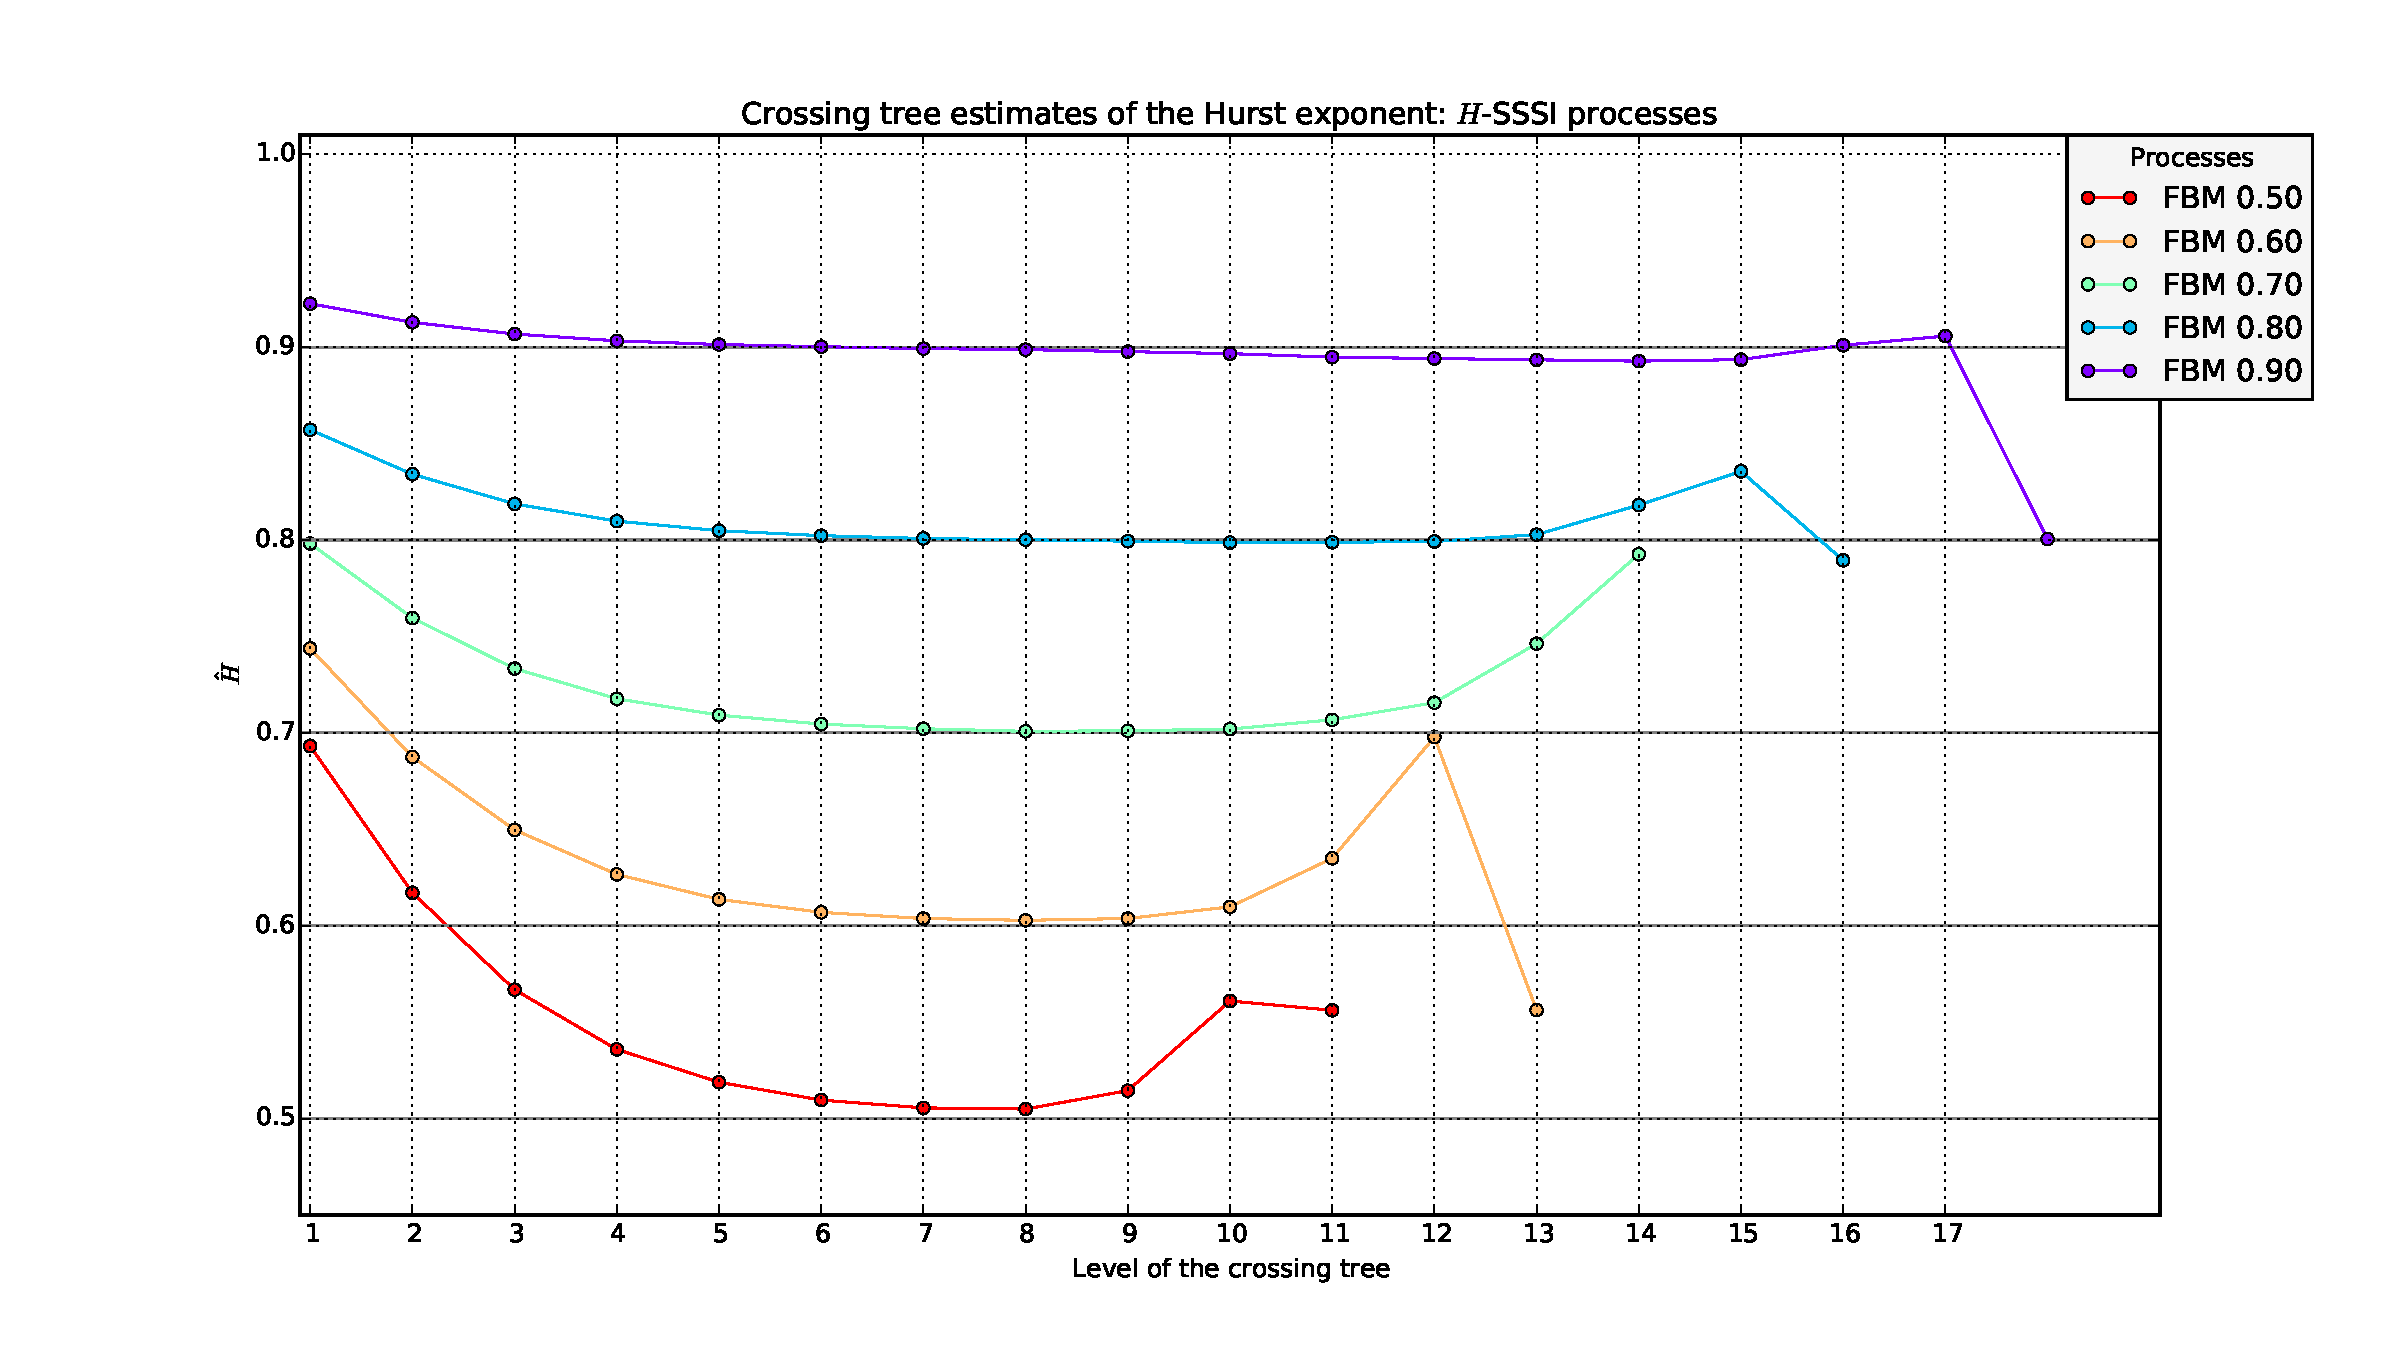
\includegraphics[width=6in]{images/fbm_fig_05_med_1000-21}
    \caption{The plot of the estimates of the Hurst index $H$ on the offspring data
    of a single level of the crossing tree based on $10^3$ Monte-Carlo simulations of
    fBm.}
\label{fig:fbm_hurst_crossing_tree}
\end{center}\end{figure}

Figure~\ref{fig:fbm_hurst_crossing_tree} suggests that scale-invariance properties
for the studied fractional processes and the chosen method of computation of the
base scale manifest their effects at across levels from 6 to 9. In fact the $\chi^2$
test described in section~\ref{sub:analysis_using_the_crossing_tree} does not seem
to support this finding and instead has the lowest empirical rejection rate exactly
at levels from 7 to 8 (see table~\ref{tbl:chi_sq_test_for_fbm_only}).
\begin{table}[h]\begin{center}
	\begin{tabular}{l||c|c|c|c|c|c|}
	Process 		&  $6-7$ &          $7-8$ & $8-9$ &  $6-8$ &  $7-9$ &  $6-9$ \\ \hline\hline
	fBm-$0.50$ 		& $10.6$ & $\mathbf{8.2}$ & $9.1$ & $13.6$ & $12.2$ & $16.2$ \\ \hline 
	fBm-$0.60$ 		& $10.9$ & $\mathbf{9.1}$ & $9.4$ & $14.2$ & $13.1$ & $16.4$ \\ \hline 
	fBm-$0.70$ 		&  $9.4$ & $\mathbf{7.0}$ & $7.2$ & $12.6$ & $11.2$ & $15.8$ \\ \hline 
	fBm-$0.80$ 		& $10.3$ & $\mathbf{6.1}$ & $6.7$ & $12.8$ & $10.7$ & $16.9$ \\ \hline 
	fBm-$0.90$ 		& $11.1$ & $\mathbf{7.8}$ & $7.9$ & $18.0$ & $12.8$ & $27.7$ \\ \hline 
 	\end{tabular}
	\caption{The table of empirical rejection rate at significance level of $\alpha = 5\%$
	of the $\chi^2$ test for self-similarity between levels of the crossing tree. }
\label{tbl:chi_sq_test_for_fbm_only}
\end{center}\end{table}
Since the self-similarity of the simulated fractional Brownian motion paths seems
to become apparent at levels 7 and 8 on average, we pool the crossing tree data of
these levels in order to obtain more reliable estimates.

Restricting the attention to the Brownian motion case (fBm with $H=\tfrac{1}{2}$)
one can easily see that the numerical evidence is well aligned with the theoretical
result of Jones and Rolls (fig.~\ref{fig:fbm_offspring_distribution}).
\begin{figure}[htb]\begin{center}
    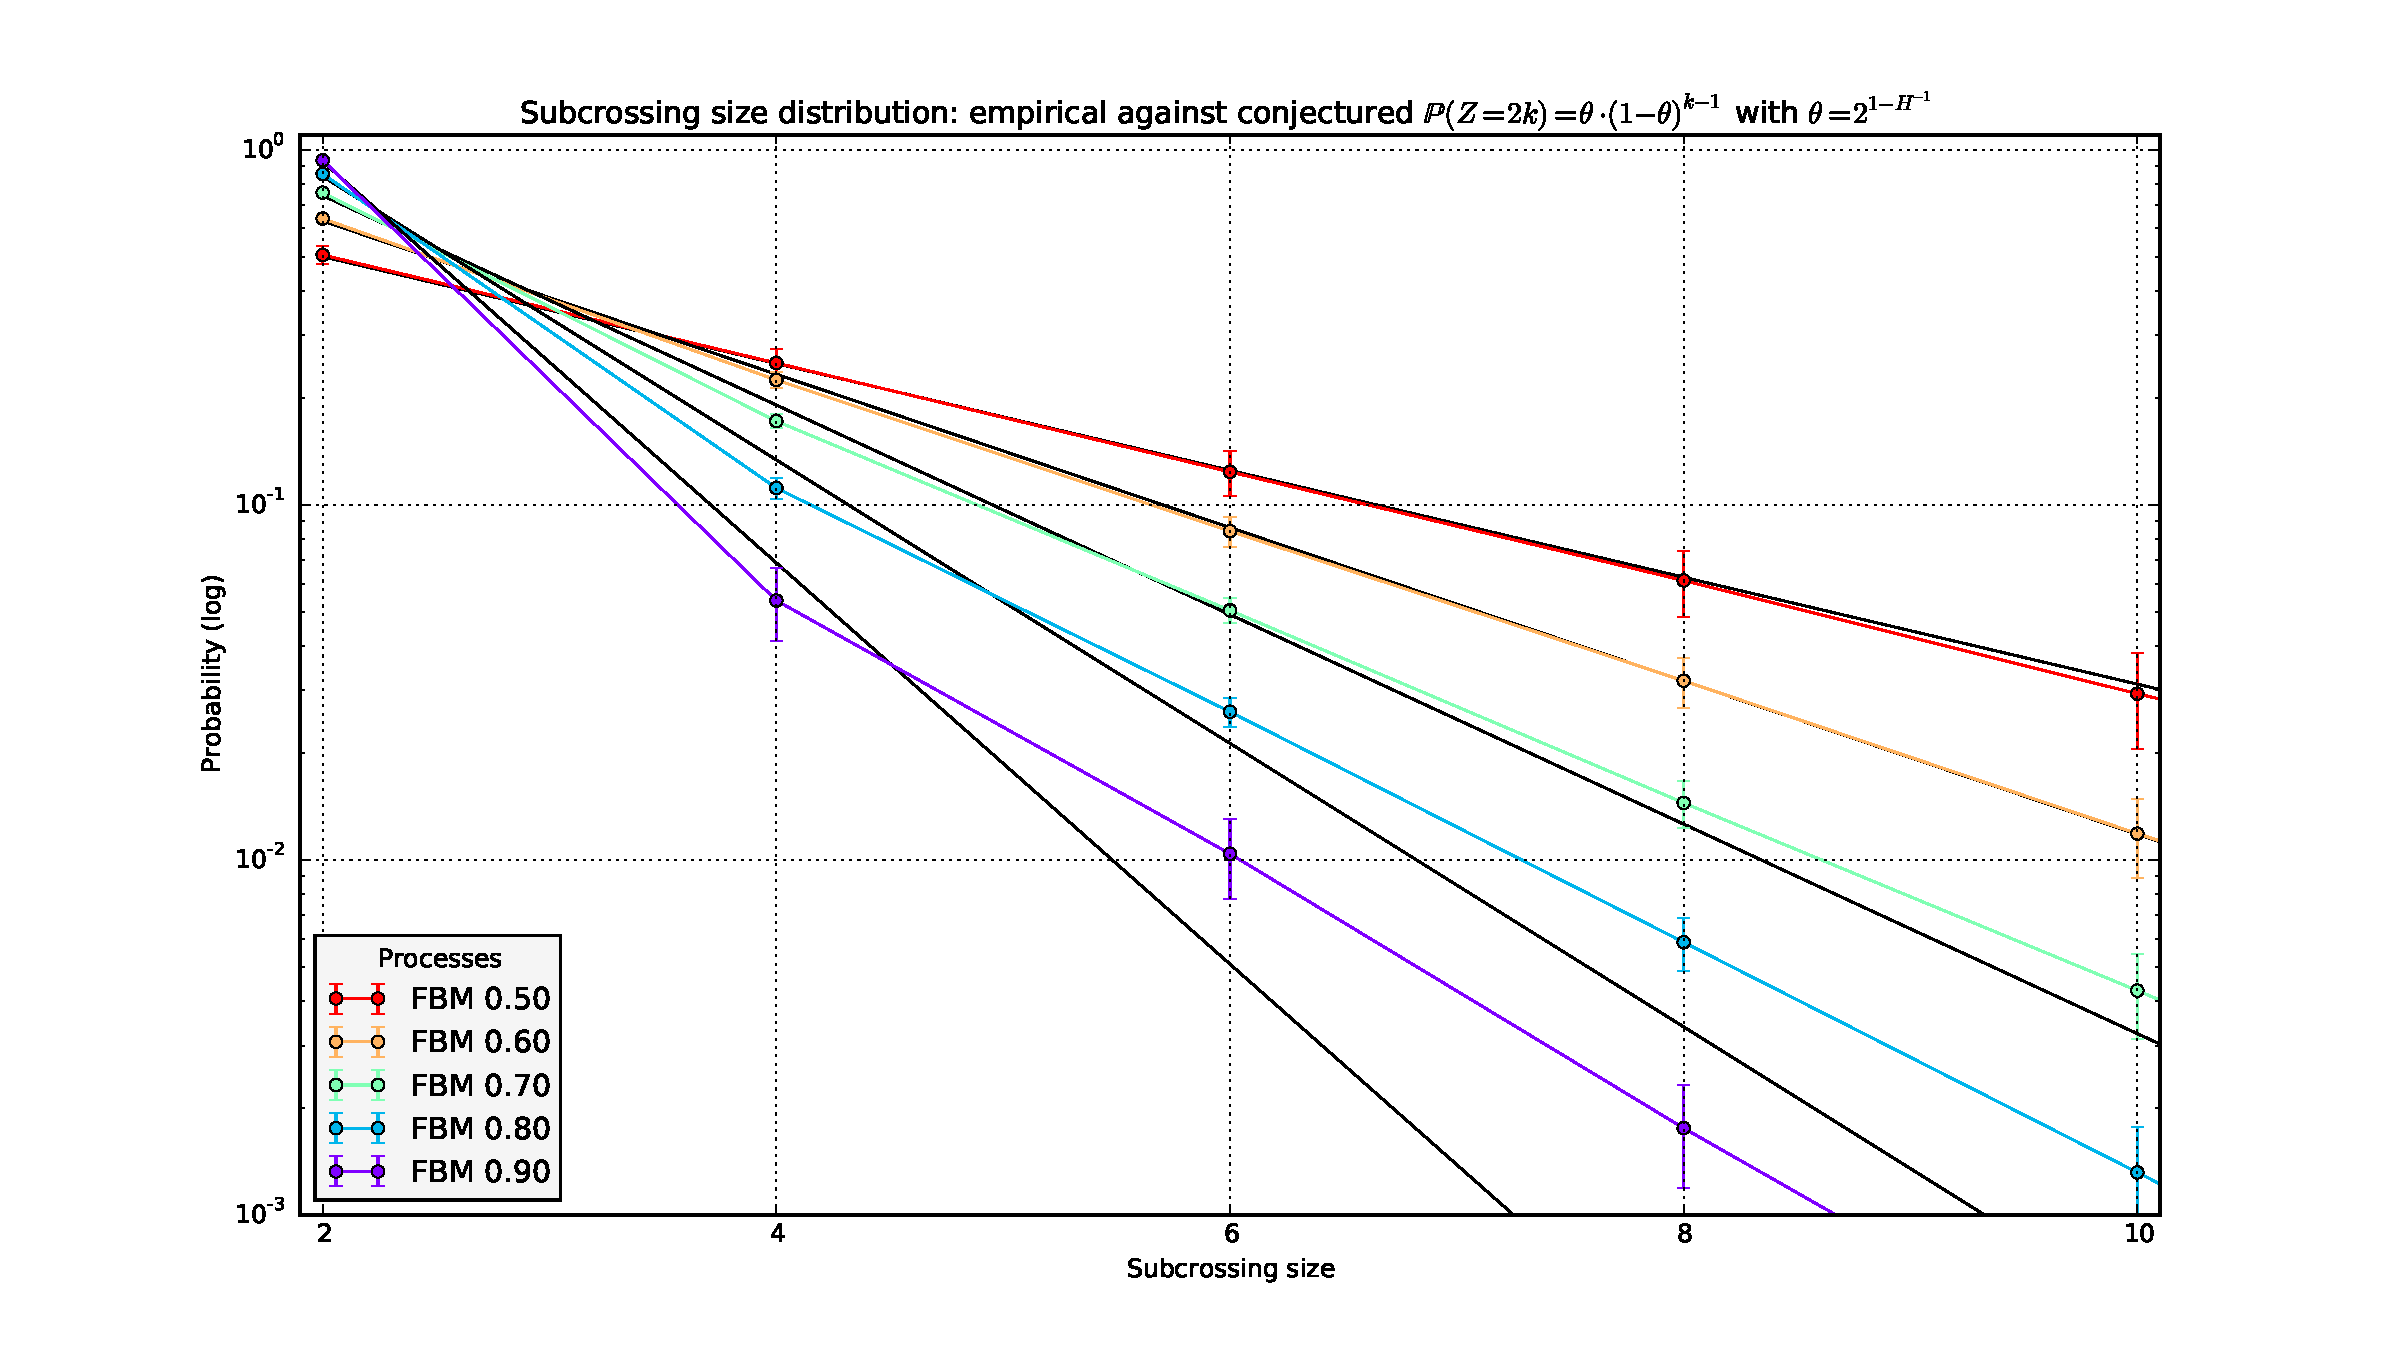
\includegraphics[width=6in]{images/fbm_fig_01_med_1000-21}
    \caption{The log-plot of the offspring distributions estimated on 1000 sample discrete paths
    of the fBm process of length $2^{21}$ and Hurst exponents in the range from $0.5$ to $0.9$.}
\label{fig:fbm_offspring_distribution}
\end{center}\end{figure}
Similarly, the theoretical probability of an up-down crossing conditional on an upcrossing
is matched very closely by the numerical evidence (fig.~\ref{fig:fbm_offspring_up_down}).
The results are similar in the down-up excursions case (fig.~\ref{fig:fbm_offspring_down_up}).

\begin{figure}[htb]\begin{center}
    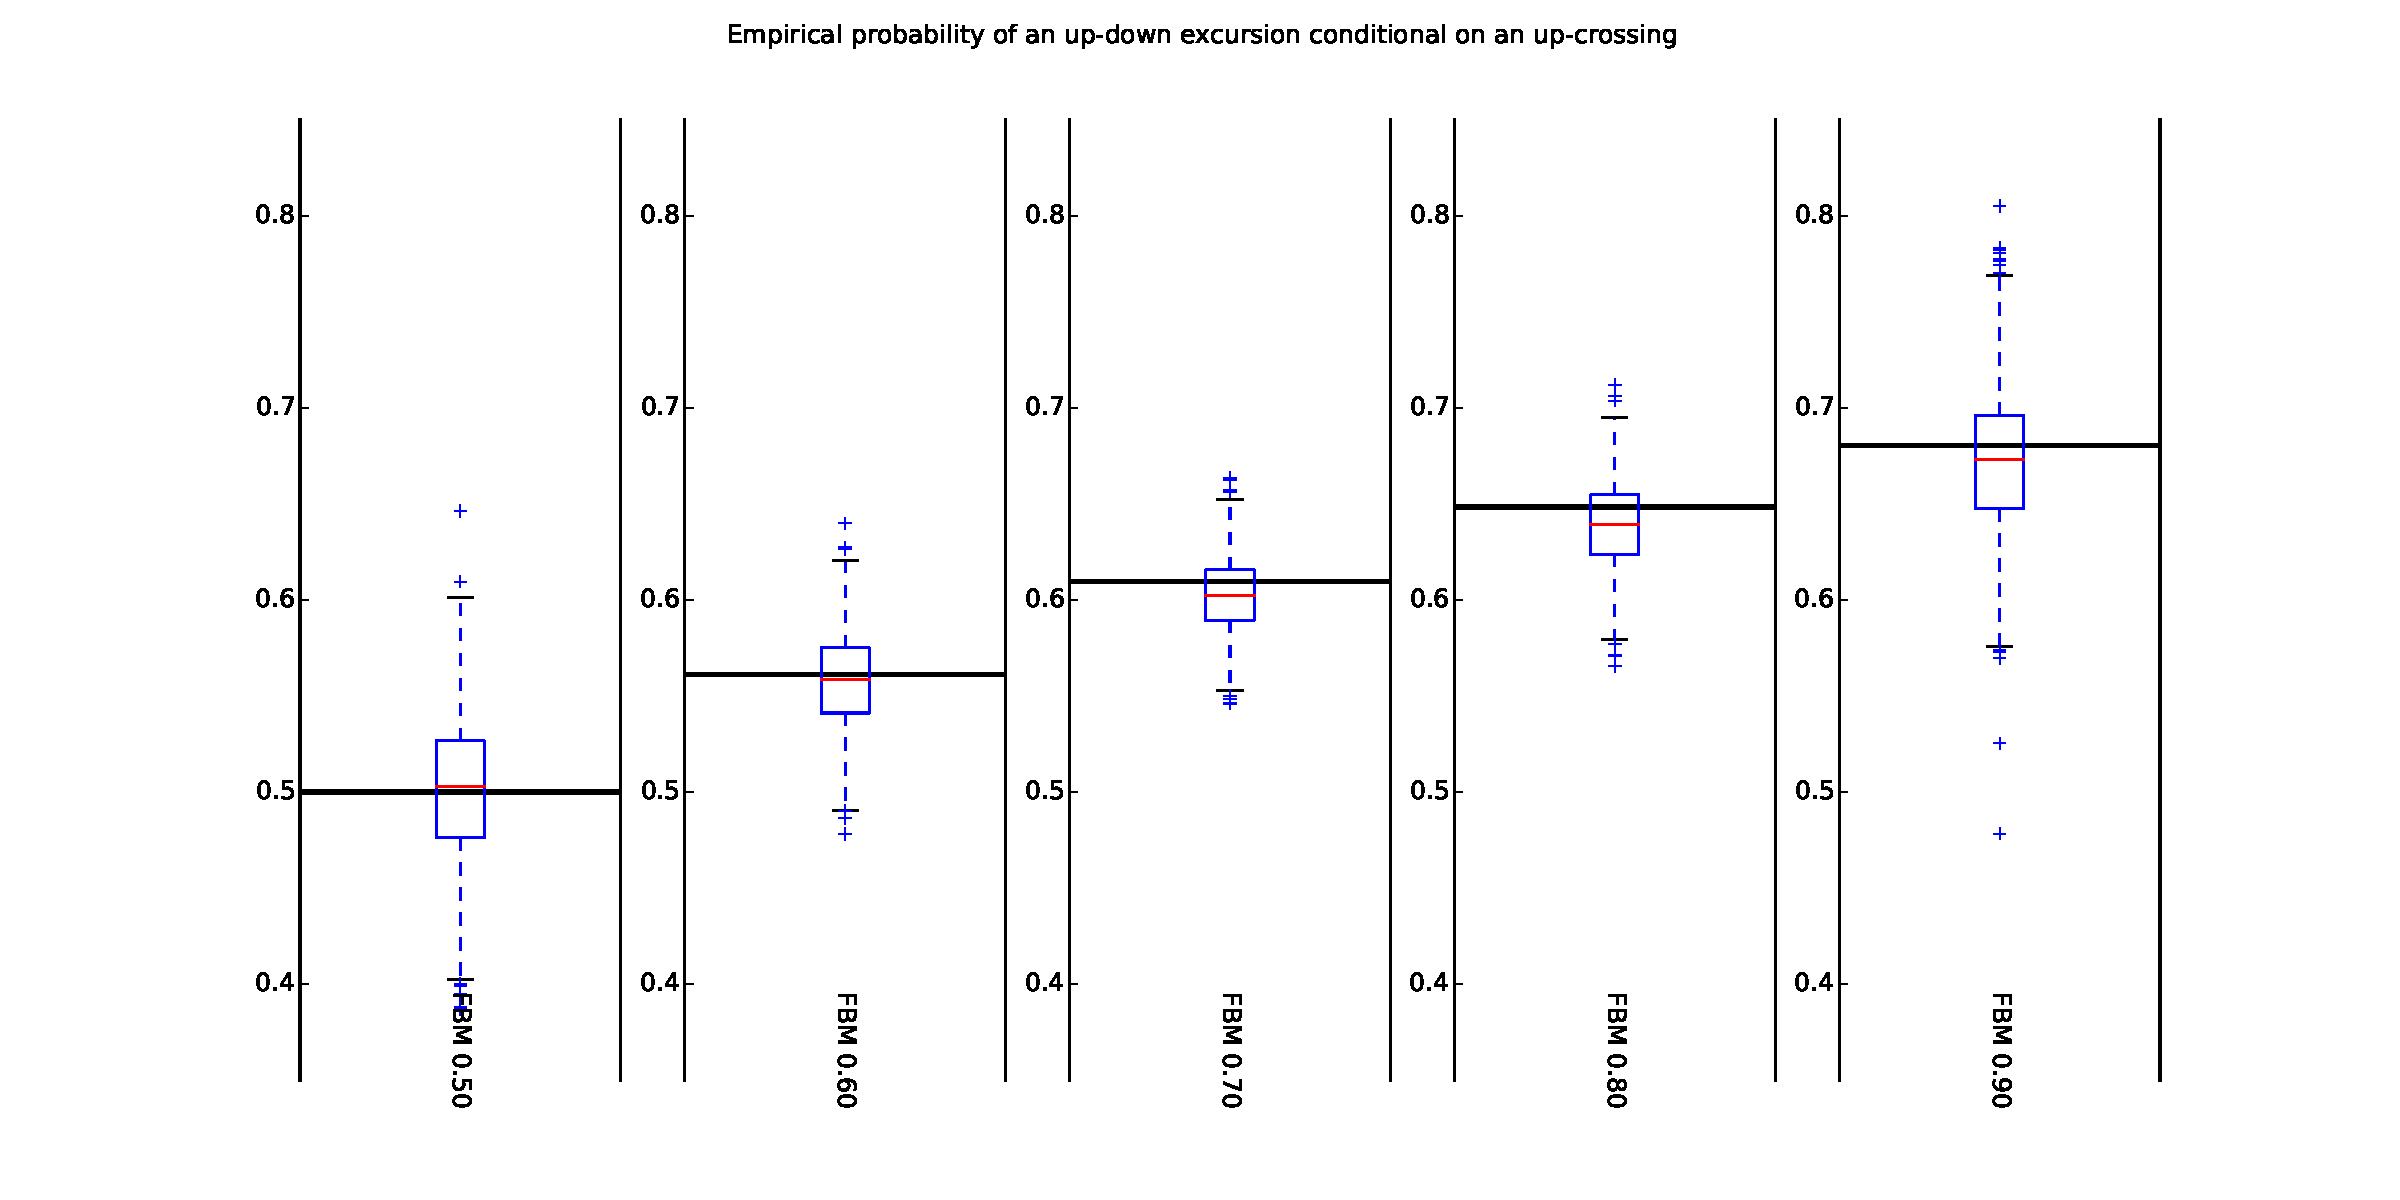
\includegraphics[width=6in]{images/fbm_fig_03_up-down_med_1000-21}
    \caption{The estimated conditional probability of an up-down excursion given upward
    orientation of the parent crossing.}
\label{fig:fbm_offspring_up_down}
\end{center}\end{figure}

\begin{figure}[htb]\begin{center}
    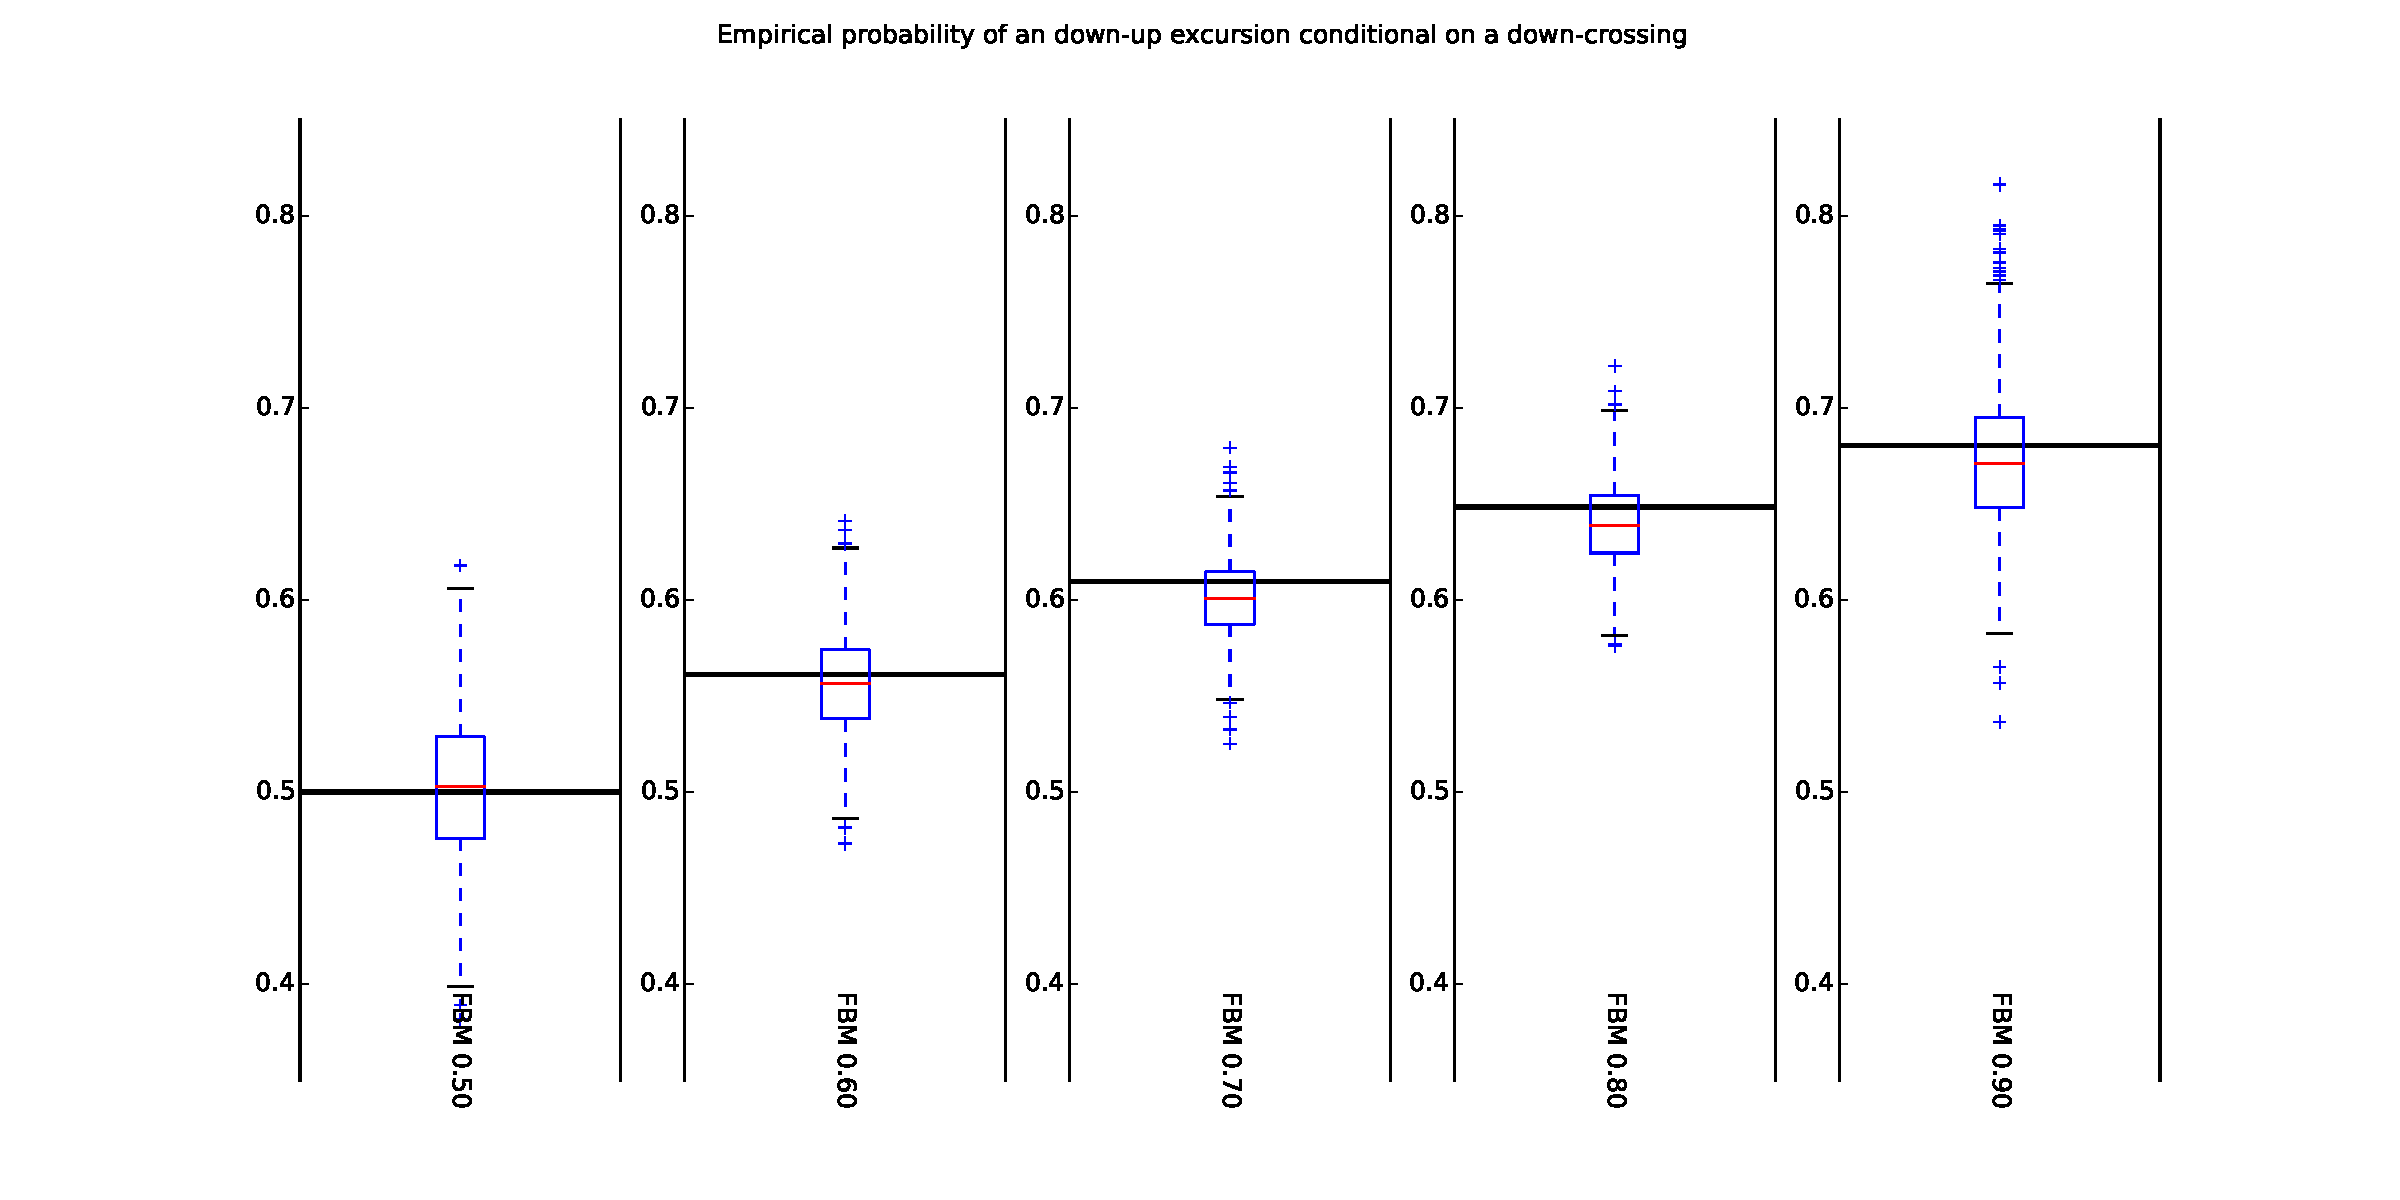
\includegraphics[width=6in]{images/fbm_fig_03_down-up_med_1000-21}
    \caption{The box-plot of the estimates of the probability of an down-up excursion
    conditional on the orientation of the parent crossing being downward.}
\label{fig:fbm_offspring_down_up}
\end{center}\end{figure}

As for the conjectured distribution, the offspring distribution in the performed
experiments seems to suggest that the levels of the tree, at least for the fractional
Brownian motion, tend to be populated by crossings with more than predicted number
of subcrossings (see tables~\ref{tbl:empirical_probs_01} for $H=0.6$
and~\ref{tbl:empirical_probs_02} for $H=0.8$). However the failure of the conjectured
crossing size distribution to match the empirical results closely, should not be
considered as a serious evidence against it in this case. Indeed, the empirical
offspring distribution for fBm with $H=0.5,0.6$ and $0.7$ is aligned quite well
with the conjecture, and since there is no theoretical reason as to why the
dependence on $H$ should break down for values of $H$ closer to $1$, we attribute
this discrepancy to numerical issues of discretizing continuous processes and
simulating fGn with long range dependence. 

Finally, the mean crossing durations, averaged for each replication across all detected
crossings of a single level indeed demonstrate plausibility of the conjectured scaling
between levels of the crossing tree, see fig.~\ref{fig:fbm_avg_crossing_durations} for fBm.
\begin{figure}[htb]\begin{center}
    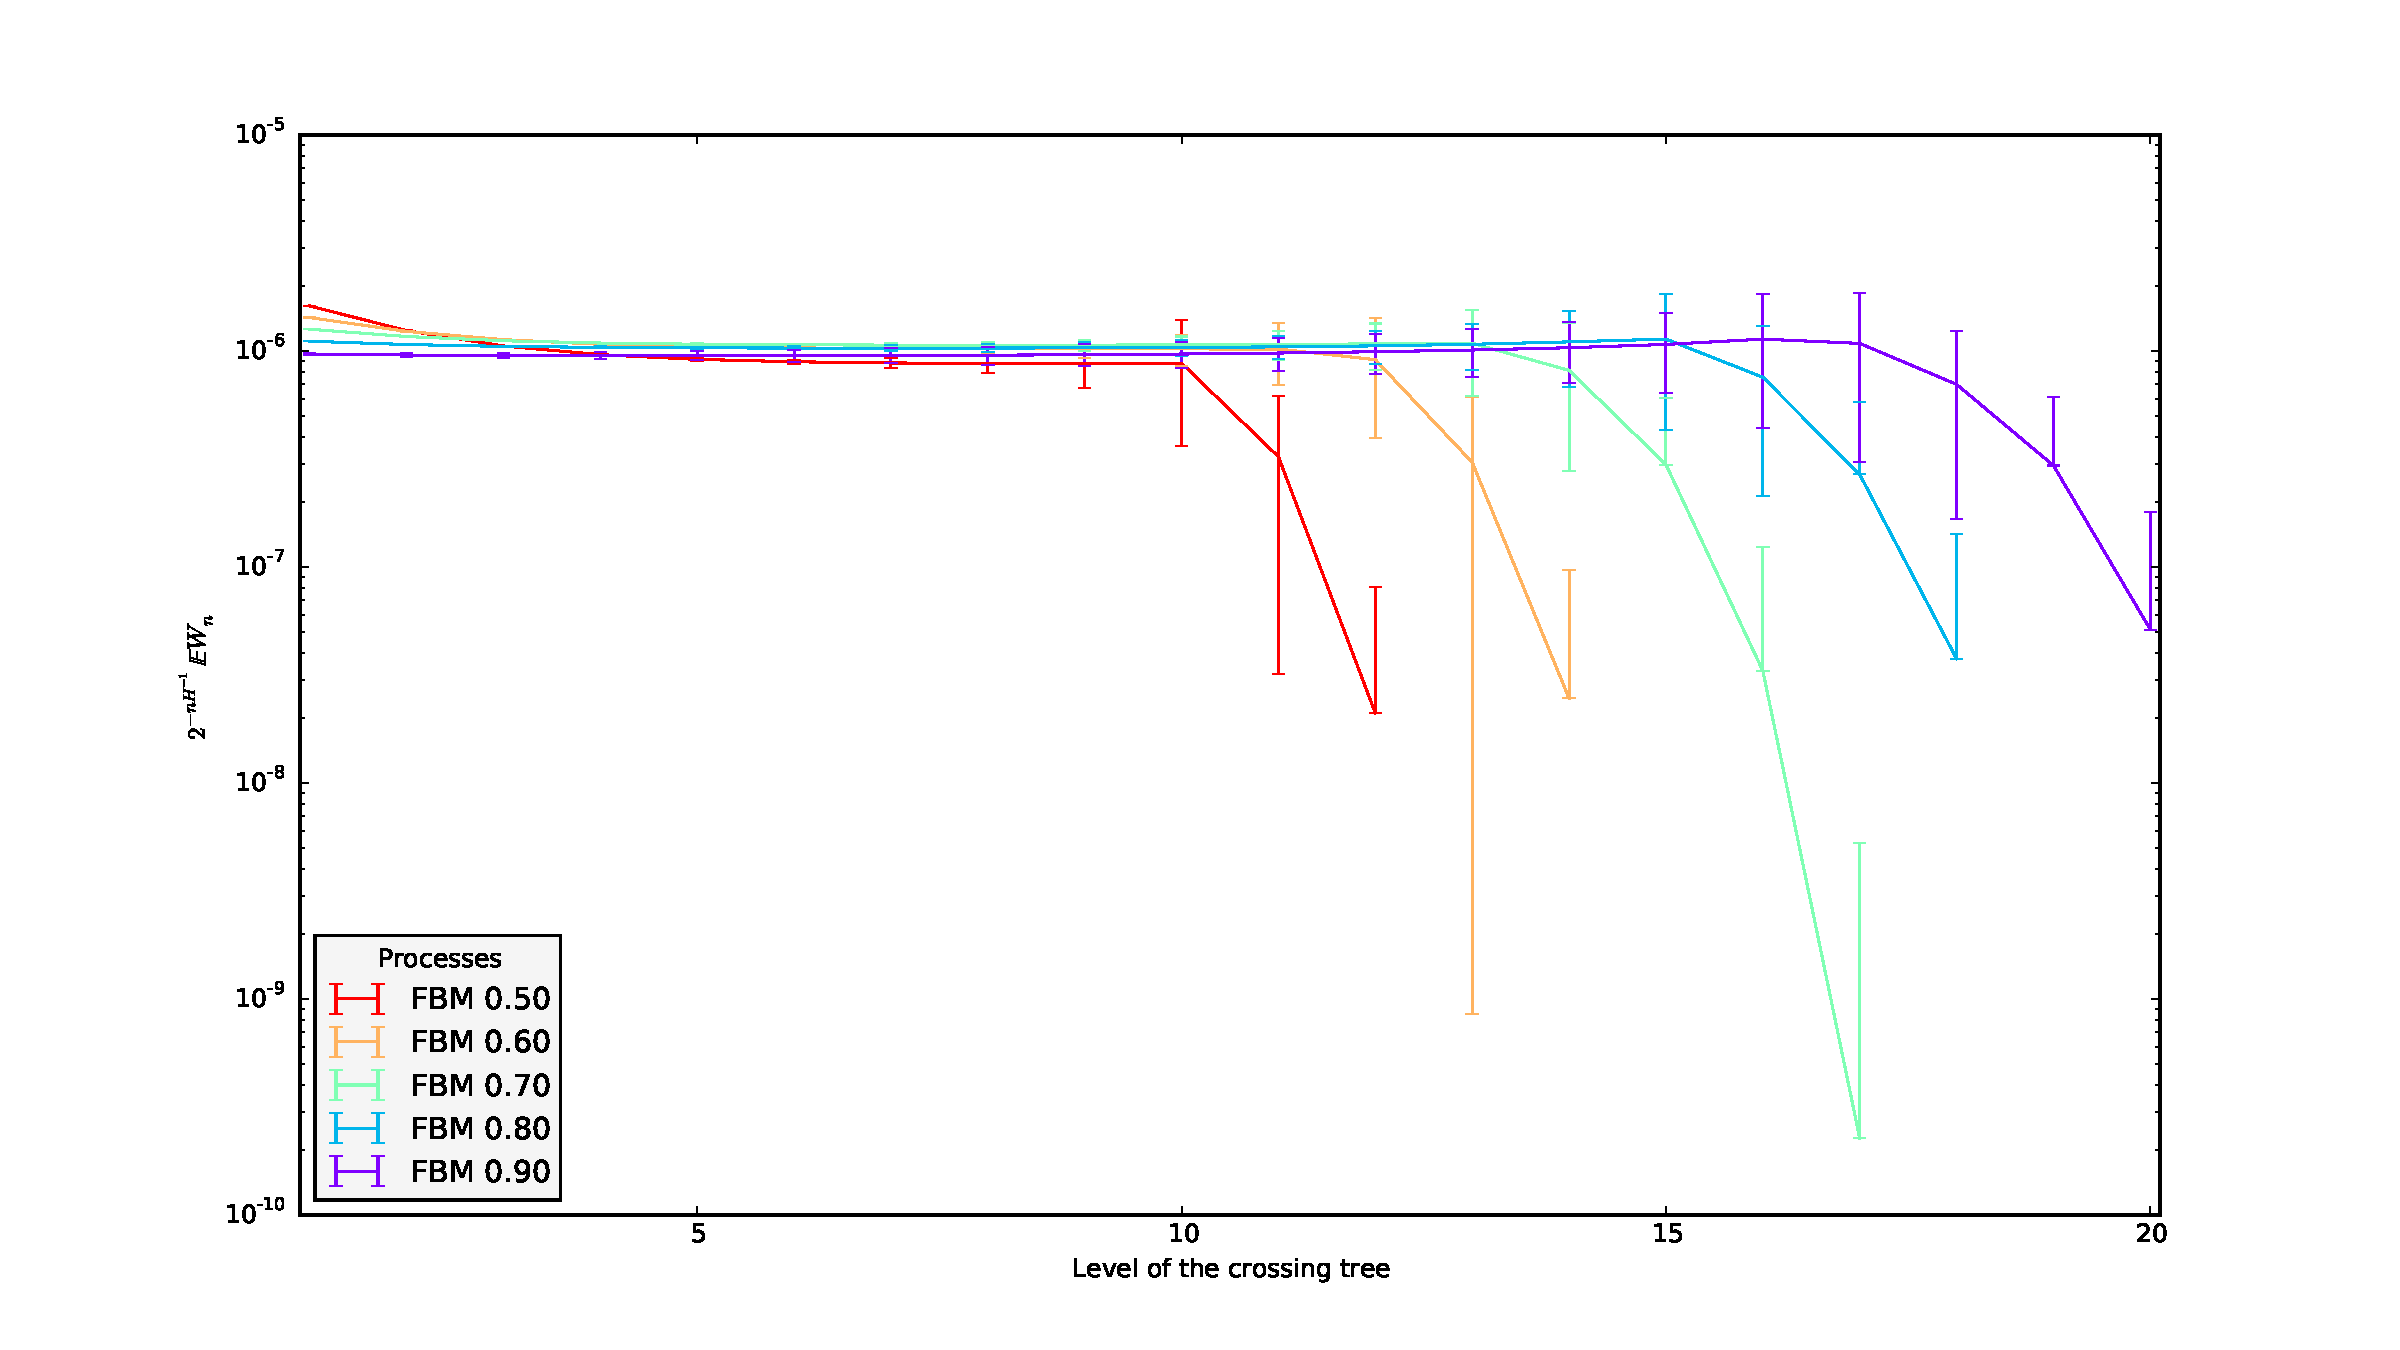
\includegraphics[width=6in]{images/fbm_fig_08_med_1000-21}
    \caption{The average crossing duration at each level of the crossing tree built
    for fractional Brownian motion processes.}
\label{fig:fbm_avg_crossing_durations}
\end{center}\end{figure}

Now let's turn to the Hermite and Weierstrass processes. This time $10^4$ random
replications of sample paths of size $2^{17}$ were generated for each process.
This size limitation was dictated by deteriorating numerical accuracy of the procedure,
responsible for generating sample paths of Hermite processes. Thus in order to produce
comparable results, sample paths of fBm and Weierstrass processes were limited to $2^{17}$
points as well.

Figure~\ref{fig:all_hurst_crossing_tree} suggests that the processes studied share common
statistical properties of the crossing tree.
\begin{figure}[htb]\begin{center}
    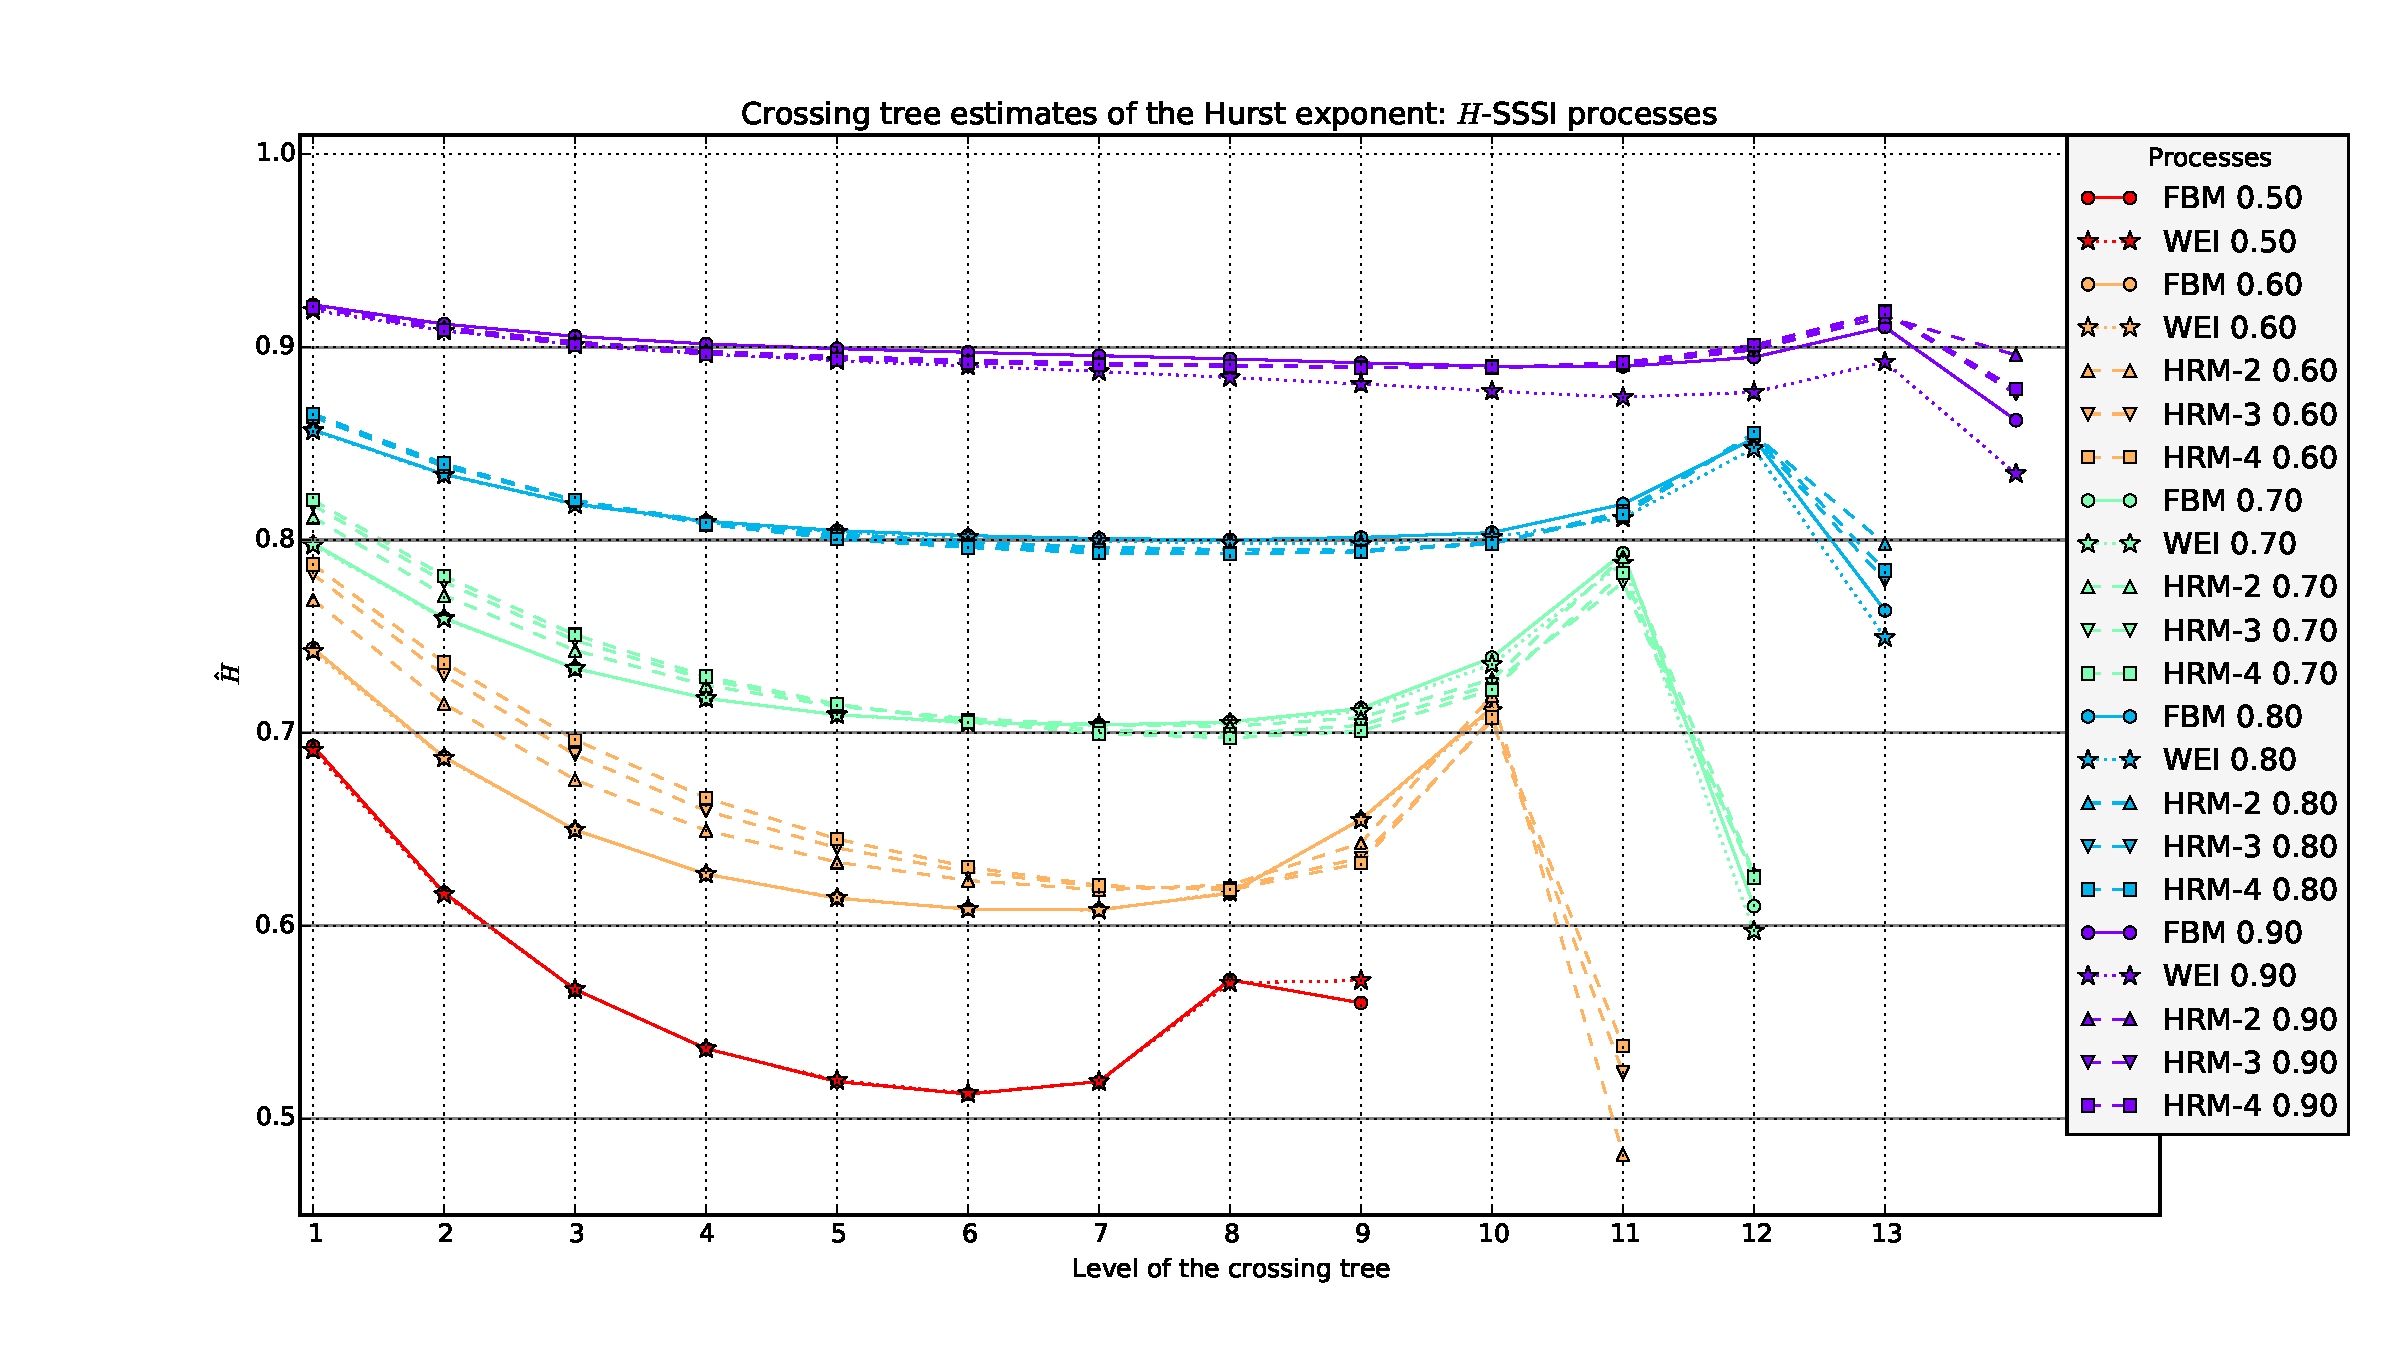
\includegraphics[width=6in]{images/fig_05_med_10000-17}
    \caption{Estimates of the Hurst exponent $H$ based on a single level of the crossing tree for
    the all studied $H$-sssi processes.}
\label{fig:all_hurst_crossing_tree}
\end{center}\end{figure}

Table~\ref{tbl:chi_sq_test_for_all_01} summarizes the empirical rejection rates of
the $\chi^2$ test for self similarity across the range of levels indicated in the
header of the table.
\begin{table}[h]\begin{center}
	\begin{tabular}{l||c|c|c|c|c|c|}
	Process 		& $6-7$ &  $7-8$ &  $8-9$ &  $6-8$ &  $7-9$ &  $6-9$ \\ \hline\hline
	  fBm-$0.50$	& $9.7$ & $15.7$ &     -- & $13.8$ &  $\mathbf{3.6}$ &  $5.4$ \\ \hline
	  fBm-$0.60$	& $8.8$ &  $9.3$ &  $\mathbf{5.6}$ & $14.2$ & $14.3$ & $16.5$ \\ \hline
	  fBm-$0.70$	& $7.6$ &  $\mathbf{6.6}$ & $10.5$ & $13.4$ & $15.7$ & $17.8$ \\ \hline
	  fBm-$0.80$	& $6.5$ &  $4.8$ &  $\mathbf{4.5}$ & $11.5$ & $13.1$ & $16.5$ \\ \hline
	  fBm-$0.90$	& $\mathbf{4.5}$ &  $5.1$ &  $6.9$ & $11.7$ & $13.6$ & $19.8$ \\ \hline\hline

	  WEI-$0.50$	& $9.6$ & $12.4$ &     -- & $13.9$ &  $\mathbf{2.2}$ &  $5.1$ \\ \hline
	  WEI-$0.60$	& $\mathbf{8.2}$ &  $9.6$ & $11.1$ & $13.2$ & $14.8$ & $15.5$ \\ \hline
	  WEI-$0.70$	& $7.0$ &  $\mathbf{5.9}$ &  $\mathbf{5.9}$ & $12.9$ & $14.6$ & $15.8$ \\ \hline
	  WEI-$0.80$	& $6.2$ &  $5.5$ &  $\mathbf{4.9}$ & $13.1$ & $13.2$ & $17.0$ \\ \hline
	  WEI-$0.90$	& $5.0$ &  $\mathbf{1.9}$ &  $8.7$ & $12.2$ &  $9.7$ & $21.0$ \\ \hline\hline

	HRM-2-$0.60$ 	& $9.6$ &  $9.2$ &  $\mathbf{7.1}$ & $15.2$ & $15.9$ & $19.6$ \\ \hline
	HRM-2-$0.70$ 	& $8.5$ &  $\mathbf{7.4}$ & $11.3$ & $13.9$ & $15.1$ & $18.2$ \\ \hline
	HRM-2-$0.80$ 	& $6.5$ &  $\mathbf{5.4}$ &  $5.6$ & $12.5$ & $12.3$ & $17.8$ \\ \hline
	HRM-2-$0.90$ 	& $6.4$ &  $\mathbf{4.9}$ &  $0.0$ & $12.7$ & $14.5$ & $18.7$ \\ \hline\hline

	HRM-3-$0.60$ 	& $9.6$ &  $\mathbf{9.2}$ & $13.7$ & $15.6$ & $17.9$ & $20.3$ \\ \hline
	HRM-3-$0.70$ 	& $\mathbf{7.9}$ &  $8.1$ &  $\mathbf{7.9}$ & $14.5$ & $16.4$ & $19.2$ \\ \hline
	HRM-3-$0.80$ 	& $5.5$ &  $\mathbf{4.3}$ &  $5.4$ & $11.8$ & $13.1$ & $16.7$ \\ \hline
	HRM-3-$0.90$ 	& $\mathbf{5.6}$ &  $7.7$ & $12.5$ & $13.4$ & $14.1$ & $19.8$ \\ \hline\hline

	HRM-4-$0.60$ 	& $9.7$ &  $\mathbf{9.3}$ & $12.3$ & $16.5$ & $17.4$ & $21.4$ \\ \hline
	HRM-4-$0.70$ 	& $8.1$ &  $7.2$ &  $\mathbf{6.0}$ & $15.4$ & $16.8$ & $20.4$ \\ \hline
	HRM-4-$0.80$ 	& $5.7$ &  $7.4$ &  $\mathbf{1.8}$ & $11.7$ & $13.7$ & $16.8$ \\ \hline
	HRM-4-$0.90$ 	& $5.1$ &  $\mathbf{2.9}$ &  $8.3$ &  $9.8$ & $12.9$ & $19.0$ \\ \hline\hline

 	\end{tabular}
	\caption{The table of empirical rejection rate at significance level of $\alpha = 5\%$
	of the $\chi^2$ test for self-similarity between levels of the crossing tree. }
\label{tbl:chi_sq_test_for_all_01}
\end{center}\end{table}
There does not seem to be a common range of levels, at the corresponding resolutions of which
all processes exhibit scale-invariance. This might be attributed to the fact that the path
of the generated processes were insufficiently long to adequately populate the higher
levels of the crossing tree. Nevertheless, it seems reasonable to expect a certain degree
of self-similarity over levels from 7 to 8, which with due caution, could yield empirical
evidence useful for analysing the conjecture.

Indeed, the offspring distribution plot (fig.~\ref{fig:all_xing_probs}) seems to
suggest that even though the theoretical distribution seems to underestimate the real
probability of a crossing of a particular size (in the number of subcrossings) as $H$
increases to $1$, there is still evidence for similarity of the statistical properties
of the crossing tree across different self-similar processes.
\begin{figure}[htb]\begin{center}
    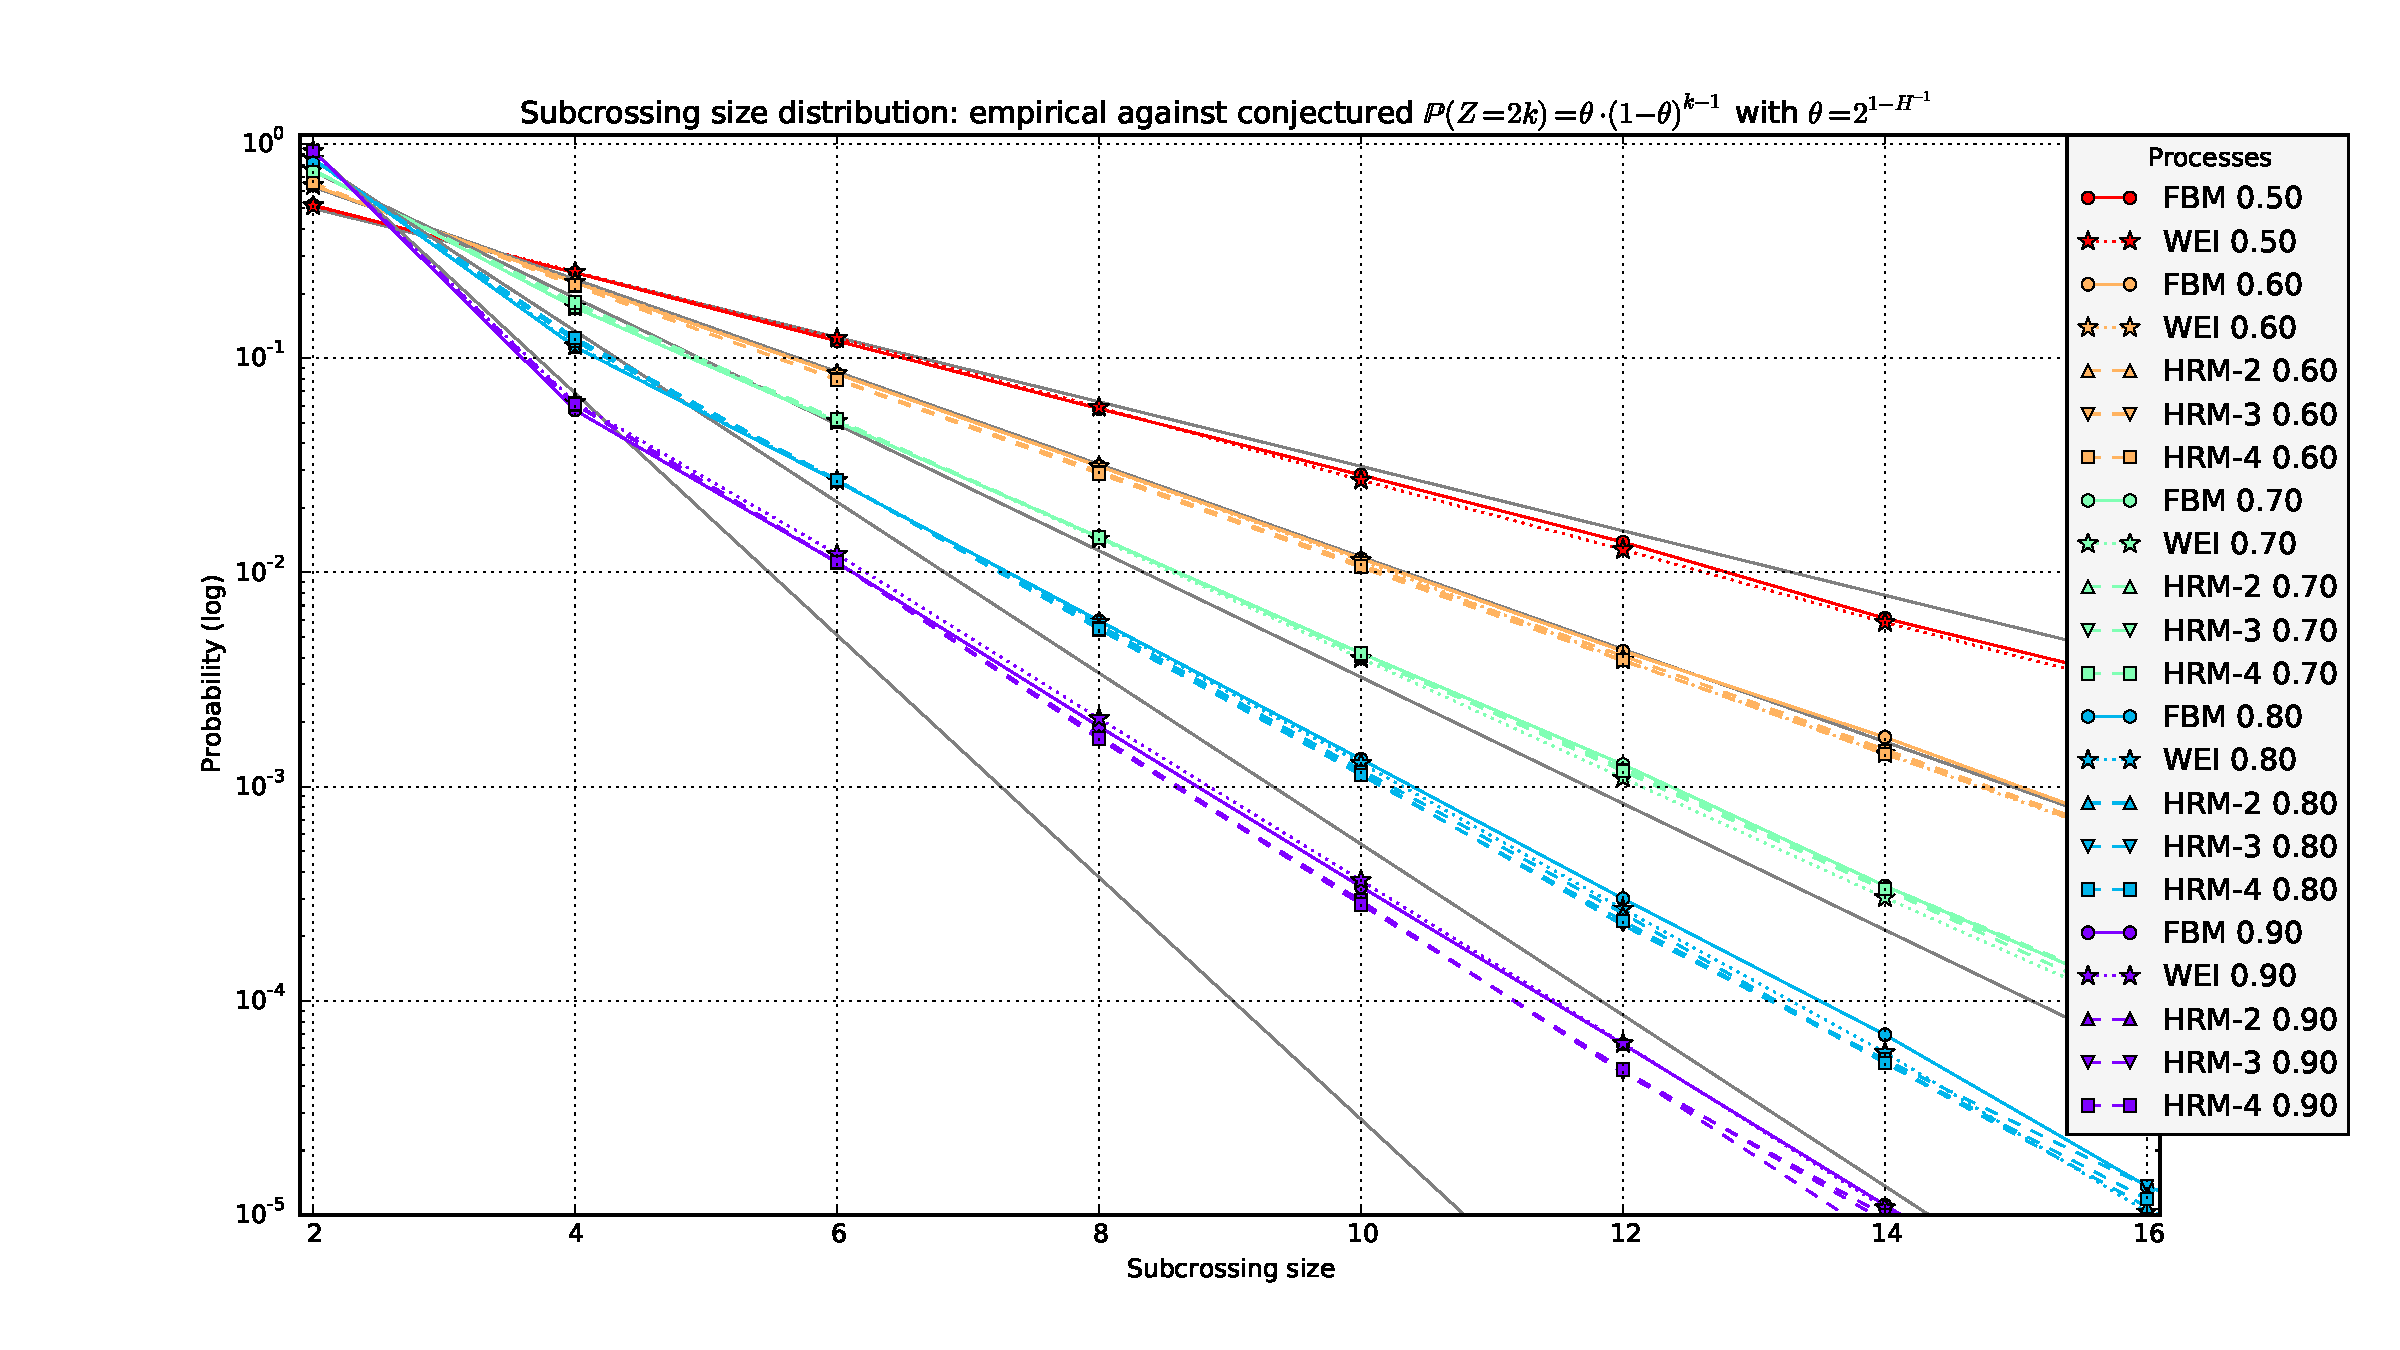
\includegraphics[width=6in]{images/fig_02_med_10000-17}
    \caption{Empirical probabilities of the crossing sizes against the hypothesized
    theoretical probabilities for $10^4$ sample paths of length $2^{17}$ points.}
\label{fig:all_xing_probs}
\end{center}\end{figure}

The tables \ref{tbl:empirical_probs_01} and \ref{tbl:empirical_probs_02} compare the 
conjectured probabilities against the empirical ones. Though there is no strong evidence
for the conjecture, one cannot say that it should be discarded. Indeed, looking at
the box-plots (\ref{fig:all_offspring_down_up} and \ref{fig:all_offspring_up_down})
of the conditional distribution of excursions, it is possible to see that even
though there is significant margin of error there the probabilities seem to agree
quite well with the hypothesised distribution.
\begin{table}[h]\begin{center}
	\begin{tabular}{l||l|l|l|l|}
					$H=0.6$ & $Z_k = 2$ & $Z_k = 4$ & $Z_k = 6$ & $Z_k = 8$ \\ \hline\hline
	\multirow{2}{*}{fBm} 	& $0.630$ & $0.233$ & $0.086$ & $0.032$ \\ \cline{2-5}
							& $0.644\pm0.033$ & $0.224\pm0.027$ & $0.083\pm0.017$ & $0.031\pm0.011$ \\ \hline\hline
	\multirow{2}{*}{WEI} 	& $0.630$ & $0.233$ & $0.086$ & $0.032$ \\ \cline{2-5}
							& $0.642\pm0.027$ & $0.226\pm0.026$ & $0.084\pm0.017$ & $0.031\pm0.010$ \\ \hline\hline
	\multirow{2}{*}{HRM-2} 	& $0.630$ & $0.233$ & $0.086$ & $0.032$ \\ \cline{2-5}
							& $0.663\pm0.034$ & $0.215\pm0.026$ & $0.078\pm0.015$ & $0.028\pm0.009$ \\ \hline\hline
	\multirow{2}{*}{HRM-3} 	& $0.630$ & $0.233$ & $0.086$ & $0.032$ \\ \cline{2-5}
							& $0.666\pm0.038$ & $0.214\pm0.026$ & $0.076\pm0.015$ & $0.027\pm0.009$ \\ \hline\hline
	\multirow{2}{*}{HRM-4} 	& $0.630$ & $0.233$ & $0.086$ & $0.032$ \\ \cline{2-5}
							& $0.667\pm0.039$ & $0.215\pm0.025$ & $0.076\pm0.016$ & $0.027\pm0.009$ \\ \hline\hline
	\end{tabular}
	\caption{The table of empirical probabilities of the first four values of the number
	of subcrossings in a parent crossing for $H$-sssi processes with $H=0.6$. Levels from
	6 to 8 were pooled to get the estimates.}
\label{tbl:empirical_probs_01}
\end{center}\end{table}

\begin{table}[h]\begin{center}
	\begin{tabular}{l||l|l|l|l|}
					$H=0.8$ & $Z_k = 2$ & $Z_k = 4$ & $Z_k = 6$ & $Z_k = 8$ \\ \hline\hline
	\multirow{2}{*}{fBm} 	& $0.841$ & $0.134$ & $0.021$ & $0.003$ \\ \cline{2-5}
 							& $0.855\pm0.023$ & $0.112\pm0.017$ & $0.026\pm0.006$ & $0.006\pm0.002$ \\ \hline\hline
	\multirow{2}{*}{HRM-2} 	& $0.841$ & $0.134$ & $0.021$ & $0.003$ \\ \cline{2-5}
 							& $0.848\pm0.027$ & $0.118\pm0.022$ & $0.026\pm0.006$ & $0.005\pm0.002$ \\ \hline\hline
	\multirow{2}{*}{HRM-3} 	& $0.841$ & $0.134$ & $0.021$ & $0.003$ \\ \cline{2-5}
 							& $0.846\pm0.024$ & $0.121\pm0.019$ & $0.026\pm0.006$ & $0.005\pm0.002$ \\ \hline\hline
	\multirow{2}{*}{HRM-4} 	& $0.841$ & $0.134$ & $0.021$ & $0.003$ \\ \cline{2-5}
 							& $0.844\pm0.021$ & $0.122\pm0.016$ & $0.026\pm0.006$ & $0.005\pm0.002$ \\ \hline\hline
	\multirow{2}{*}{WEI} 	& $0.841$ & $0.134$ & $0.021$ & $0.003$ \\ \cline{2-5}
 							& $0.854\pm0.019$ & $0.113\pm0.015$ & $0.026\pm0.005$ & $0.006\pm0.002$ \\ \hline\hline
	\end{tabular}
	\caption{The table of empirical probabilities of the first four values of the number
	of subcrossings in a parent crossing for $H$-sssi processes with $H=0.8$. Levels from
	6 to 8 were pooled to get the estimates.}
\label{tbl:empirical_probs_02}
\end{center}\end{table}

Crossing duration also do not seem contradict the hypothesized scaling for $H$-sssi
processes and the Weierstrass function (see fig.~\ref{fig:wei_durations} - \ref{fig:hrm_4_durations}).
Also we considered the properly scaled empirical quantiles (not presented here) of
the crossing durations between the processes considered and across all sufficiently
populated levels (from $1$-st to $10$-th) of the sample crossing tree. The conclusion
is that there is indeed similarity (up to a multiplicative constant depending on
the base scale $\delta$) of the crossing durations' distribution among processes
(see fig.~\ref{fig:fbm_quantiles_06}, \ref{fig:fbm_quantiles_08} and \ref{fig:fbm_quantiles_durations}).

\begin{figure}[htb]\begin{center}
    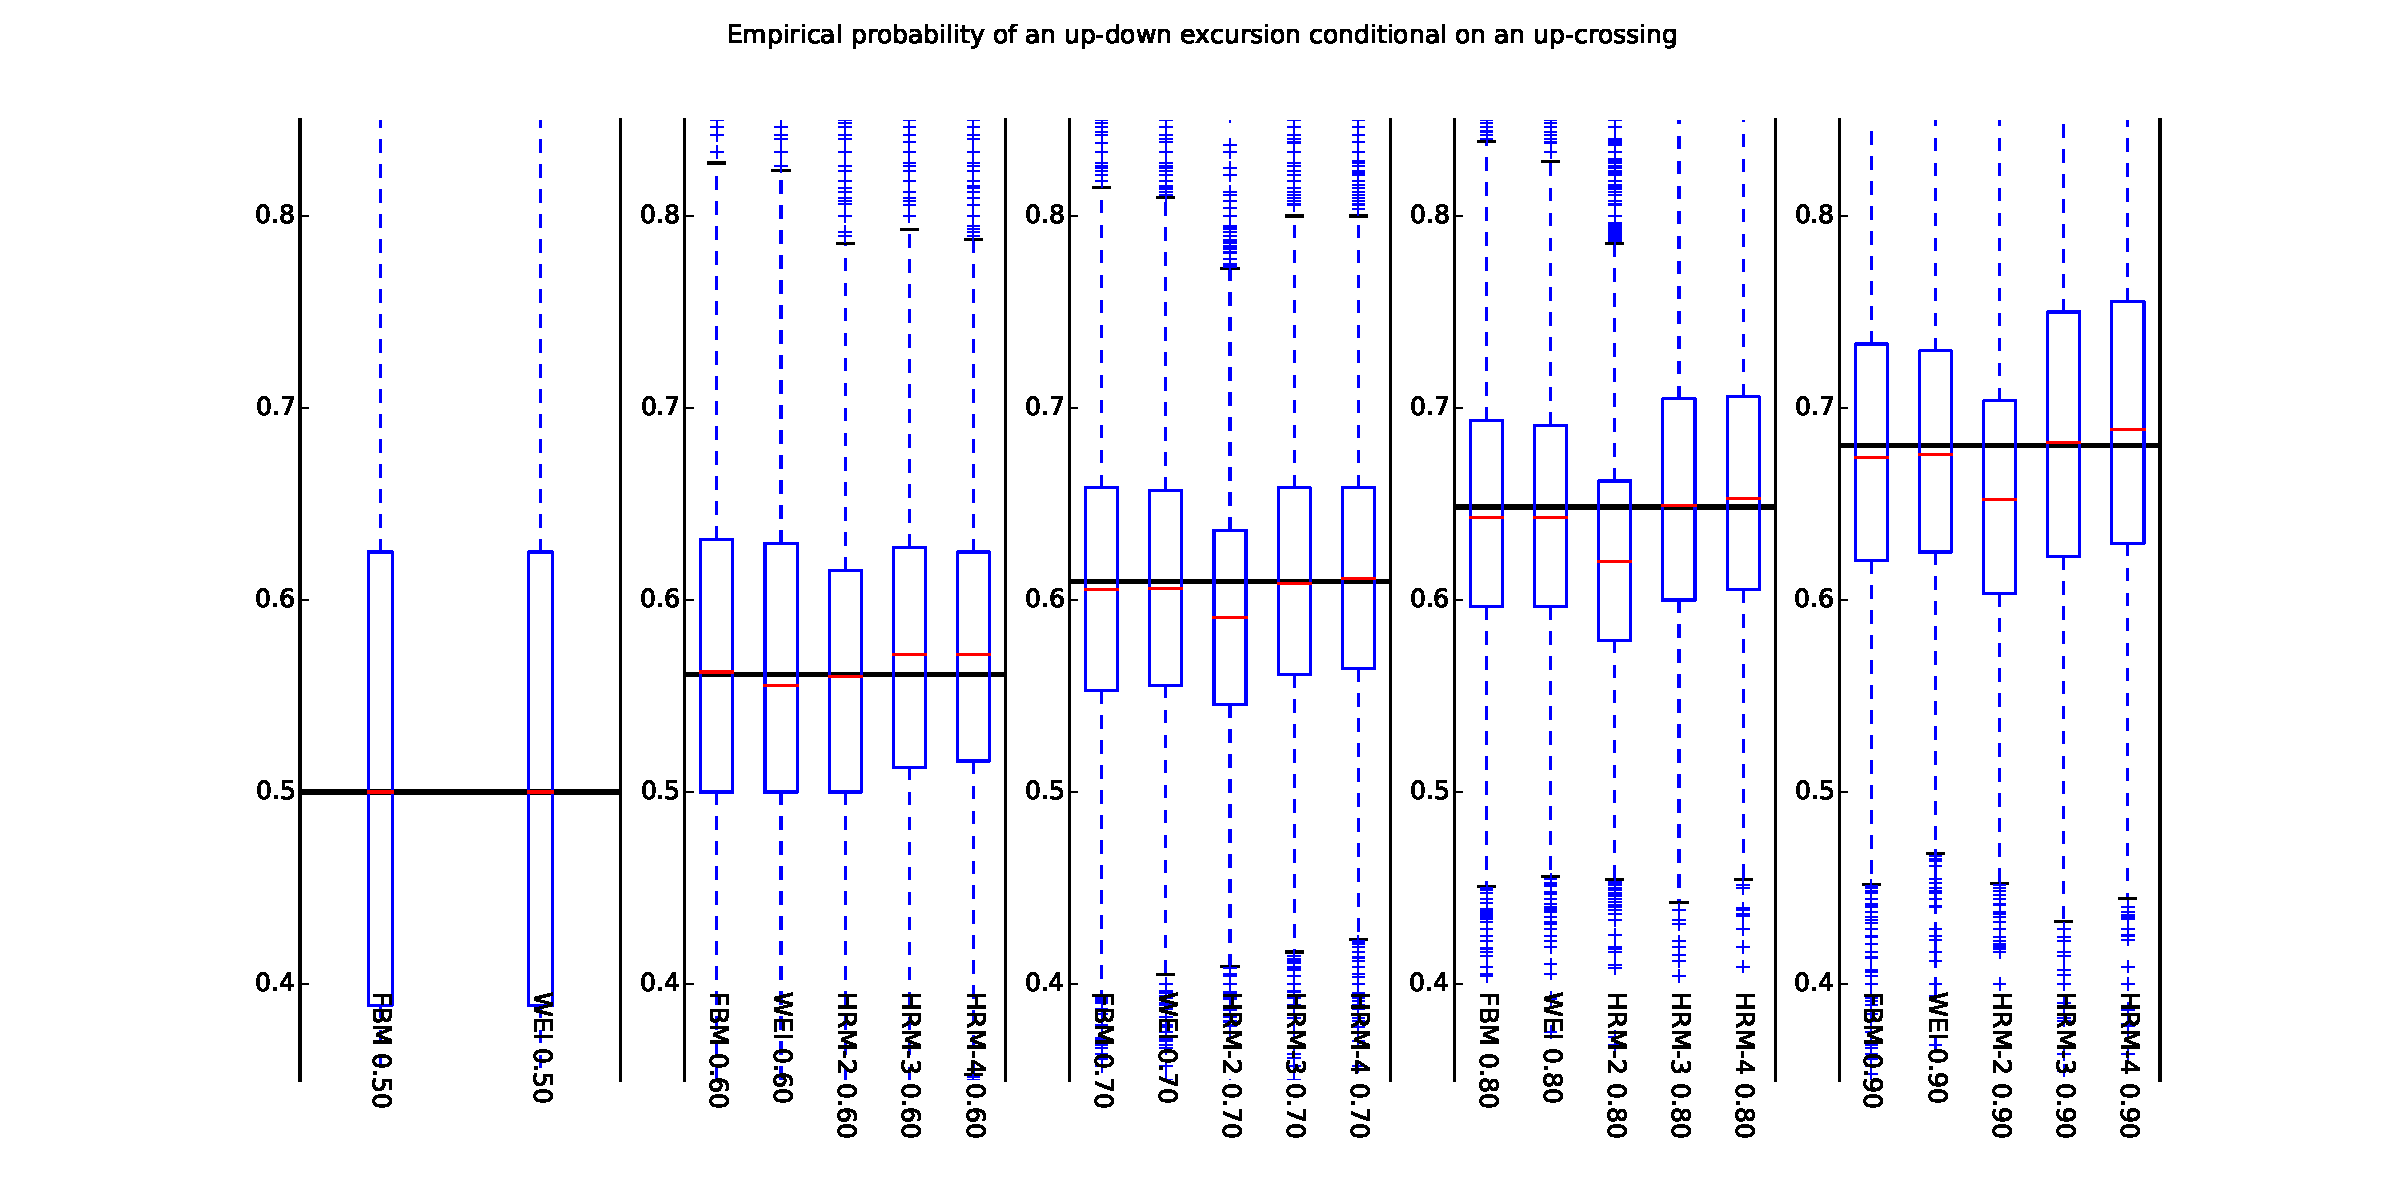
\includegraphics[width=6in]{images/fig_03_up-down_med_10000-17}
    \caption{The empirical estimates of the probability of an up-down excursion conditional on
    the upward orientation of the parent crossing.}
\label{fig:all_offspring_up_down}
\end{center}\end{figure}

\begin{figure}[htb]\begin{center}
    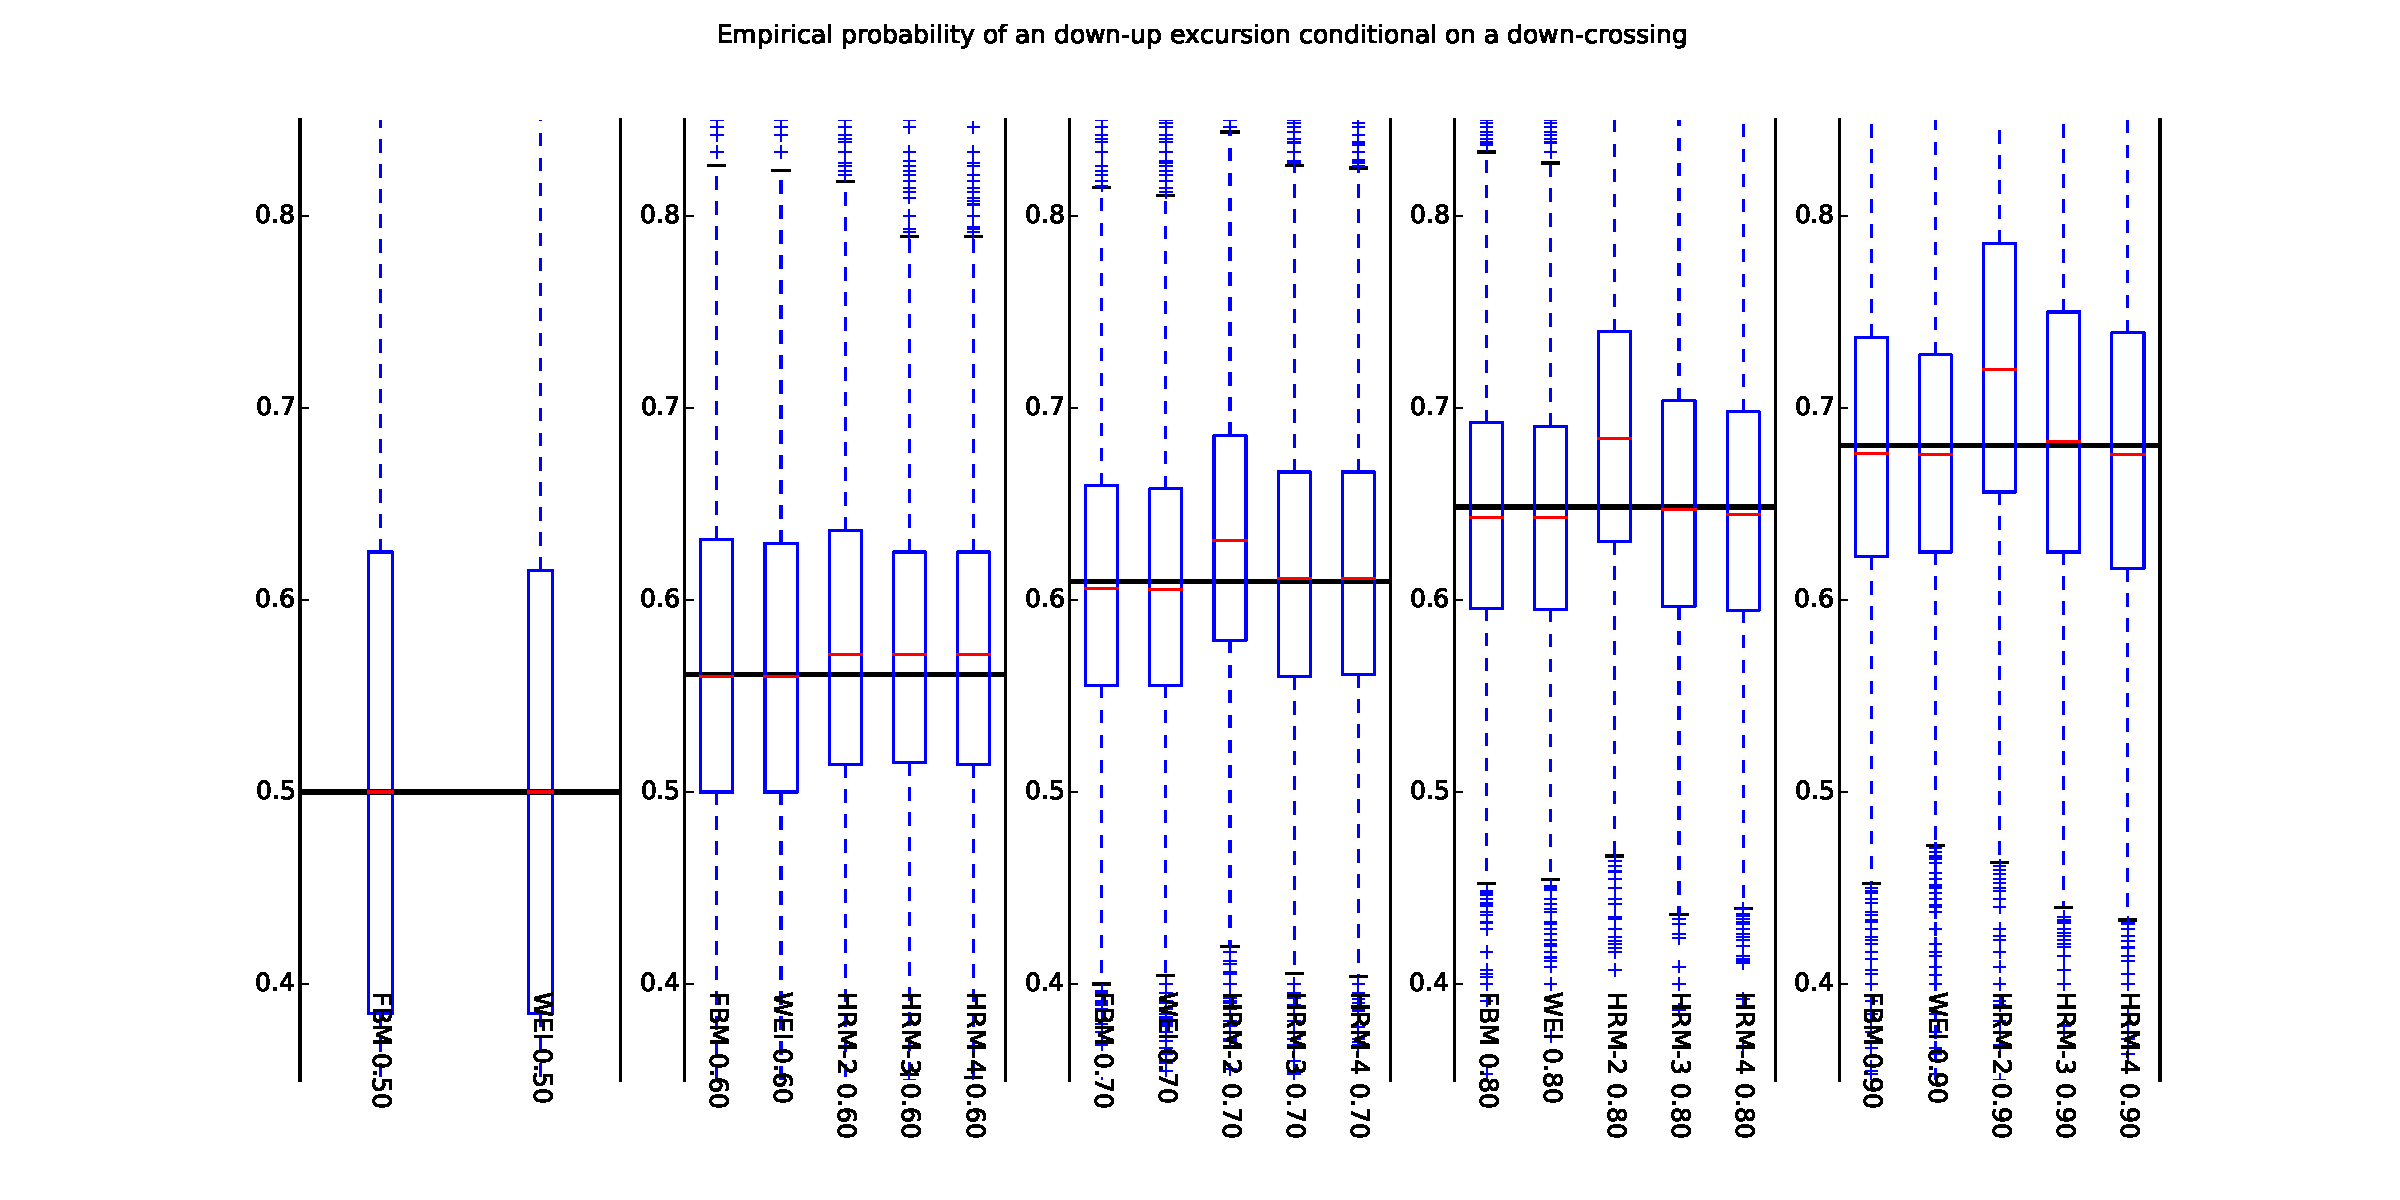
\includegraphics[width=6in]{images/fig_03_down-up_med_10000-17}
    \caption{The same figure as~\ref{fig:all_offspring_up_down} but for down-up excursions
    conditional on the orientation of the parent crossing being downward.}
\label{fig:all_offspring_down_up}
\end{center}\end{figure}

\begin{figure}[htb]\begin{center}
    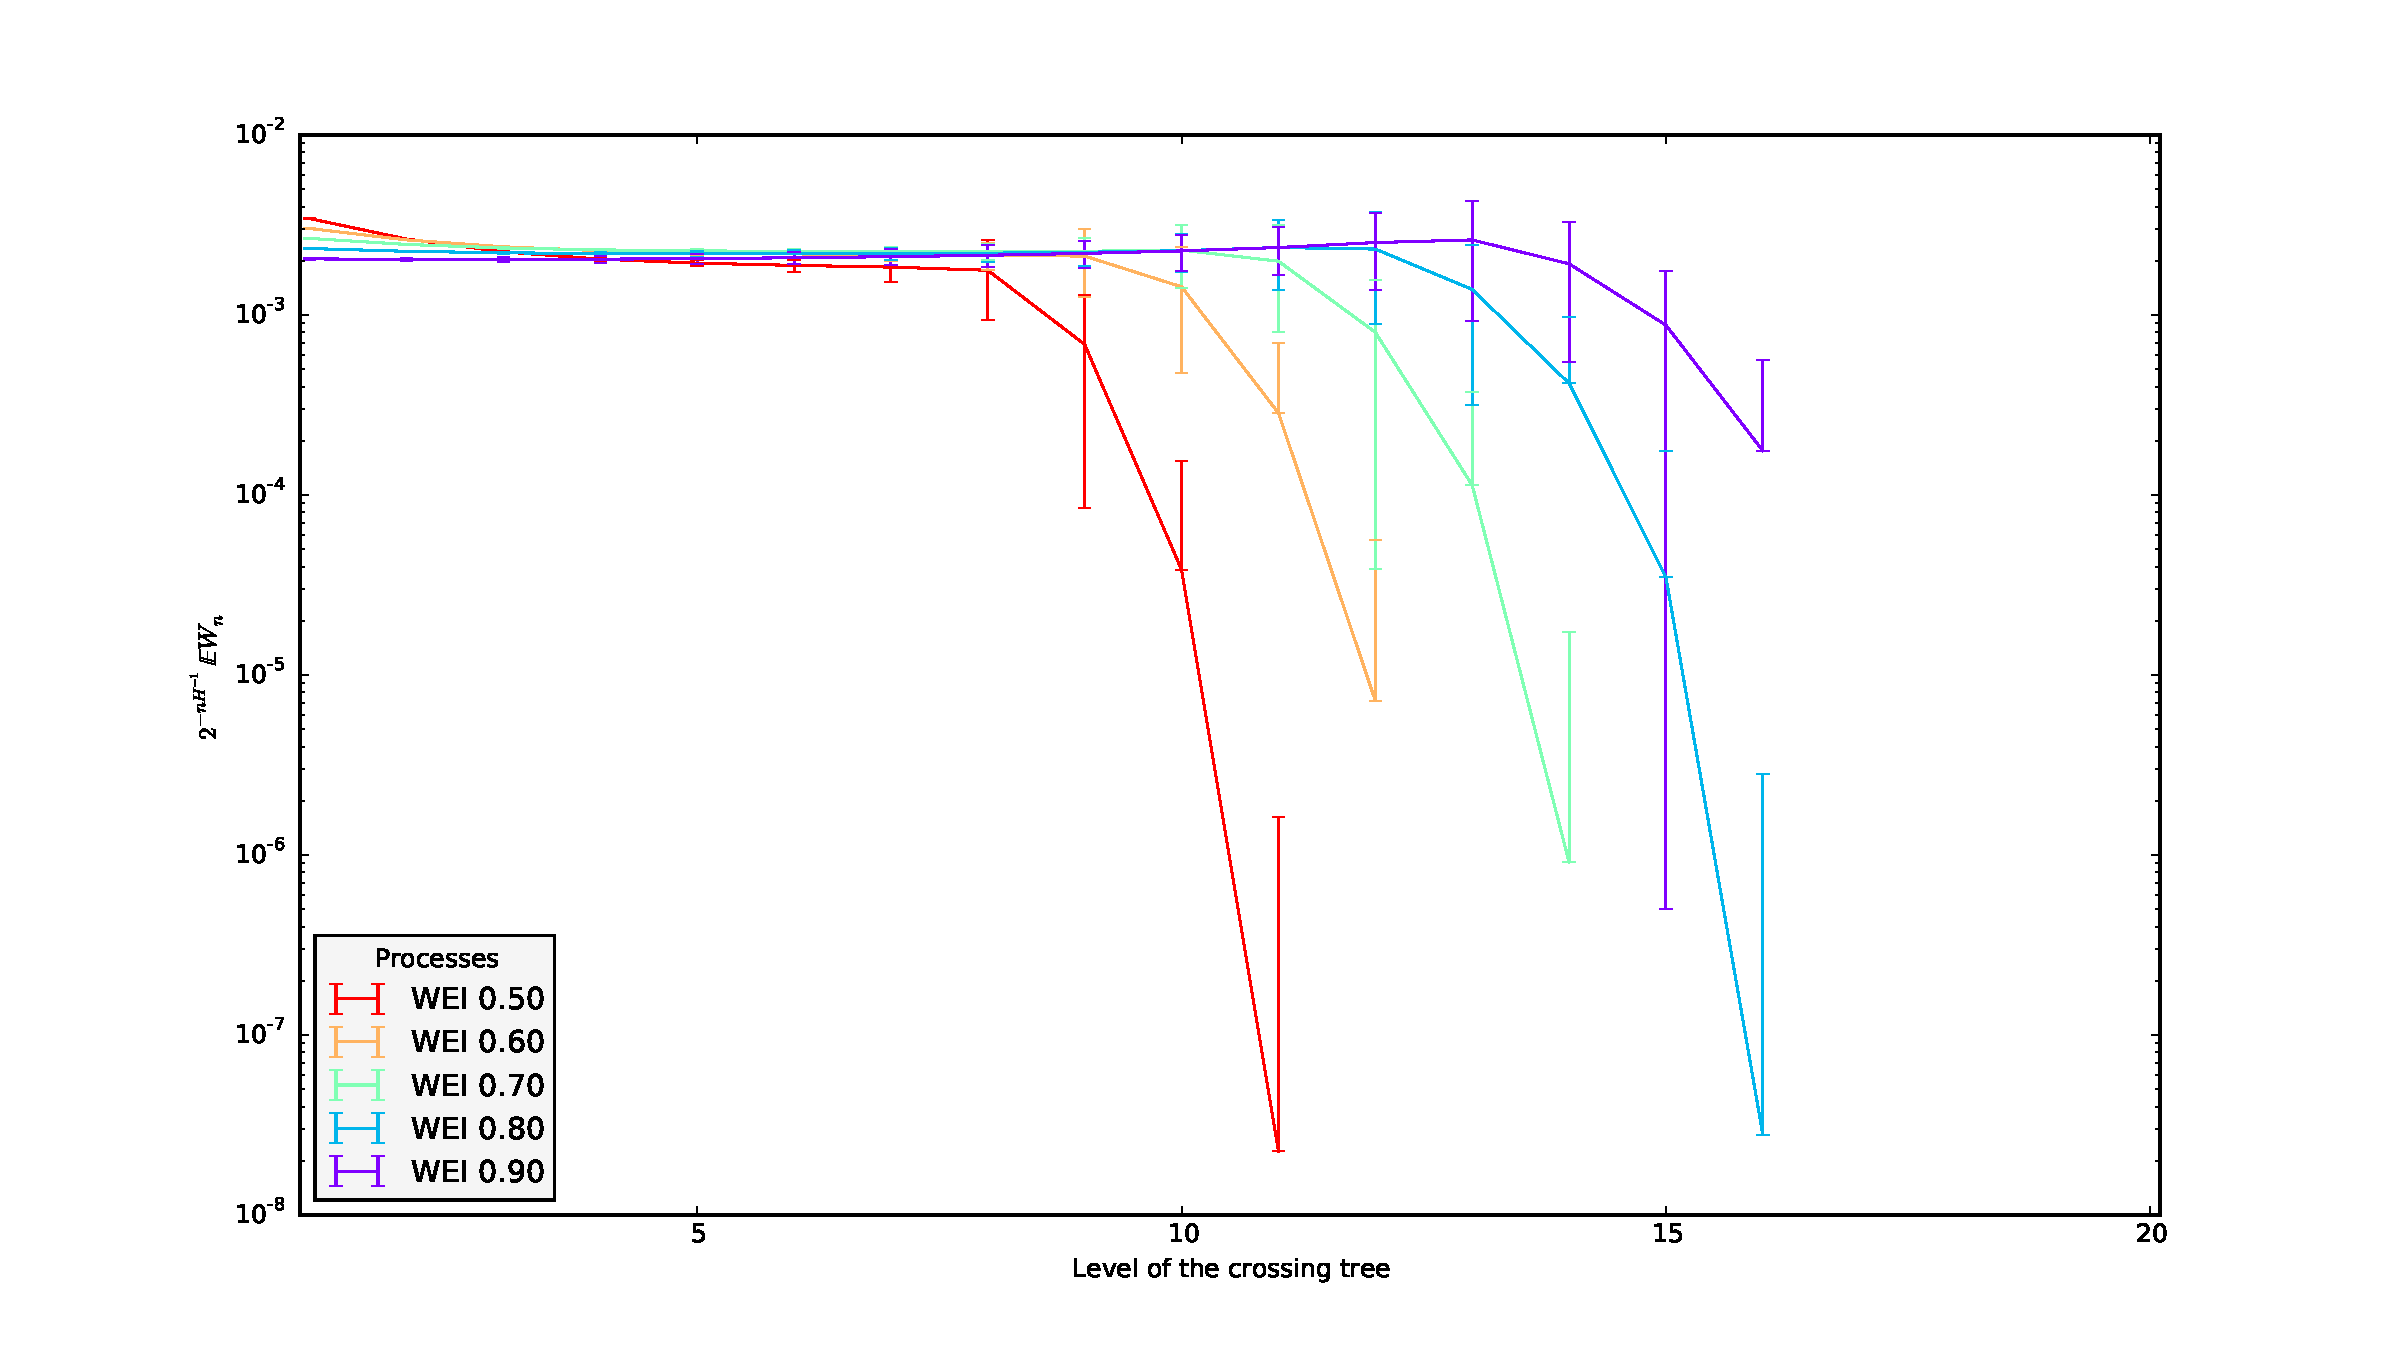
\includegraphics[width=6in]{images/fig_08_med_WEI_10000-17}
    \caption{The average crossing duration at each level of the crossing tree built
    for the Weierstrass processes.}
\label{fig:wei_durations}
\end{center}\end{figure}

\begin{figure}[htb]\begin{center}
    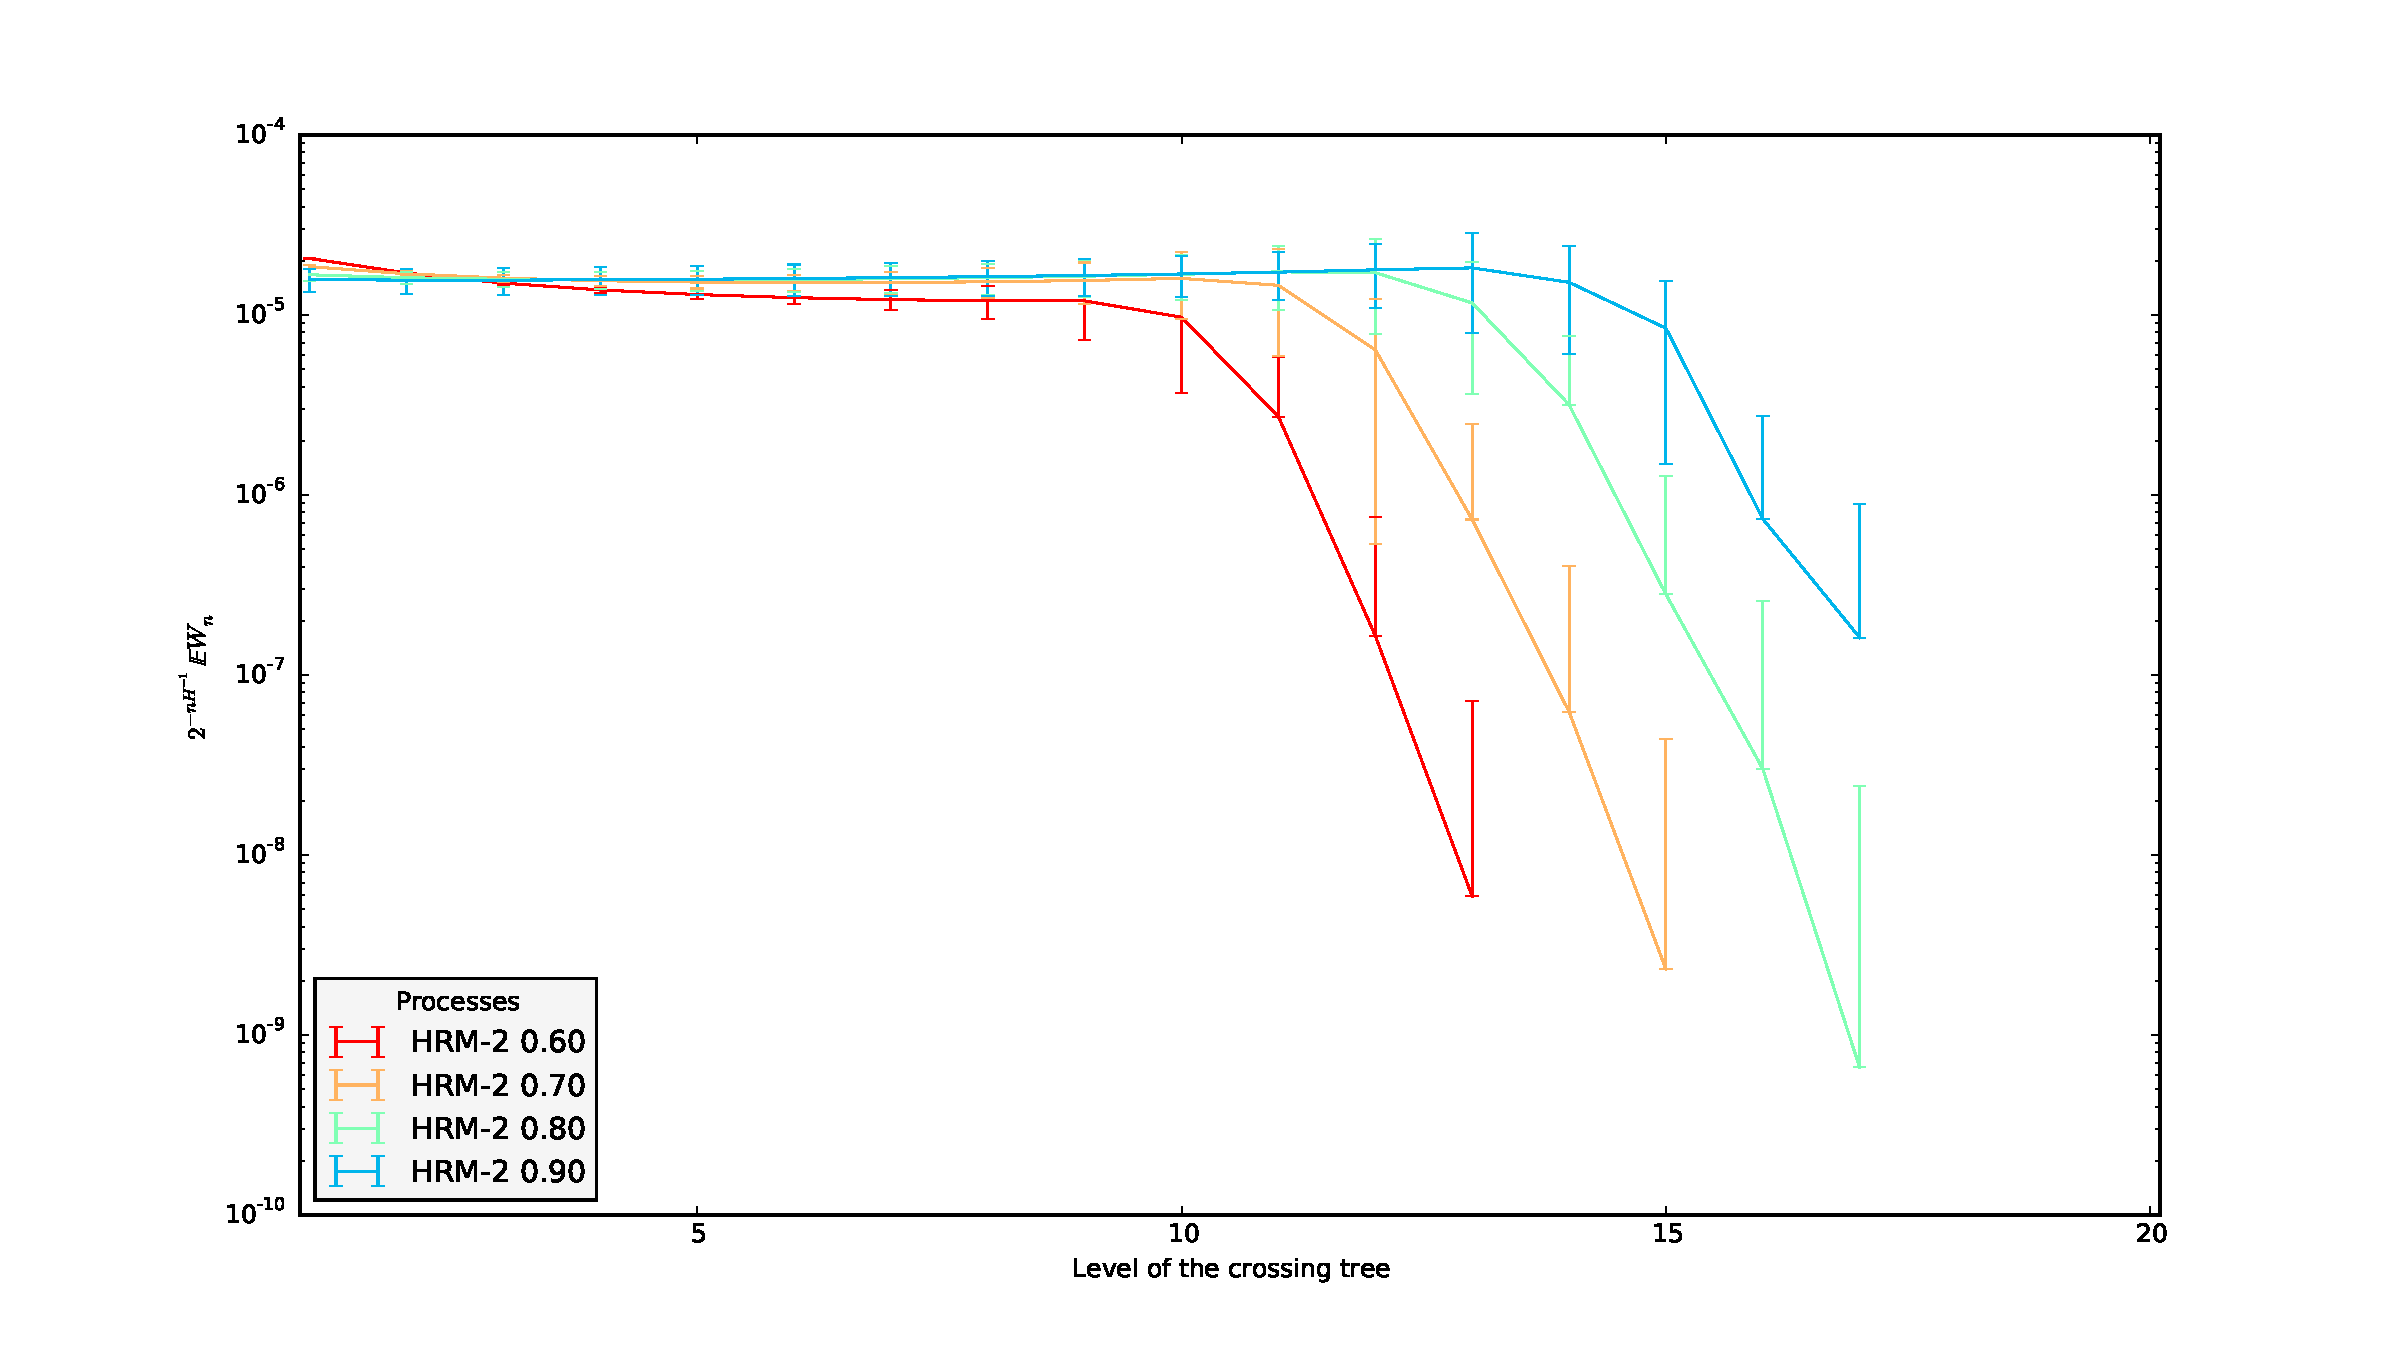
\includegraphics[width=6in]{images/fig_08_med_HRM-2_10000-17}
    \caption{The average crossing duration at each level of the crossing tree built
    for the Hermite processes of order $2$.}
\label{fig:hrm_2_durations}
\end{center}\end{figure}

\begin{figure}[htb]\begin{center}
    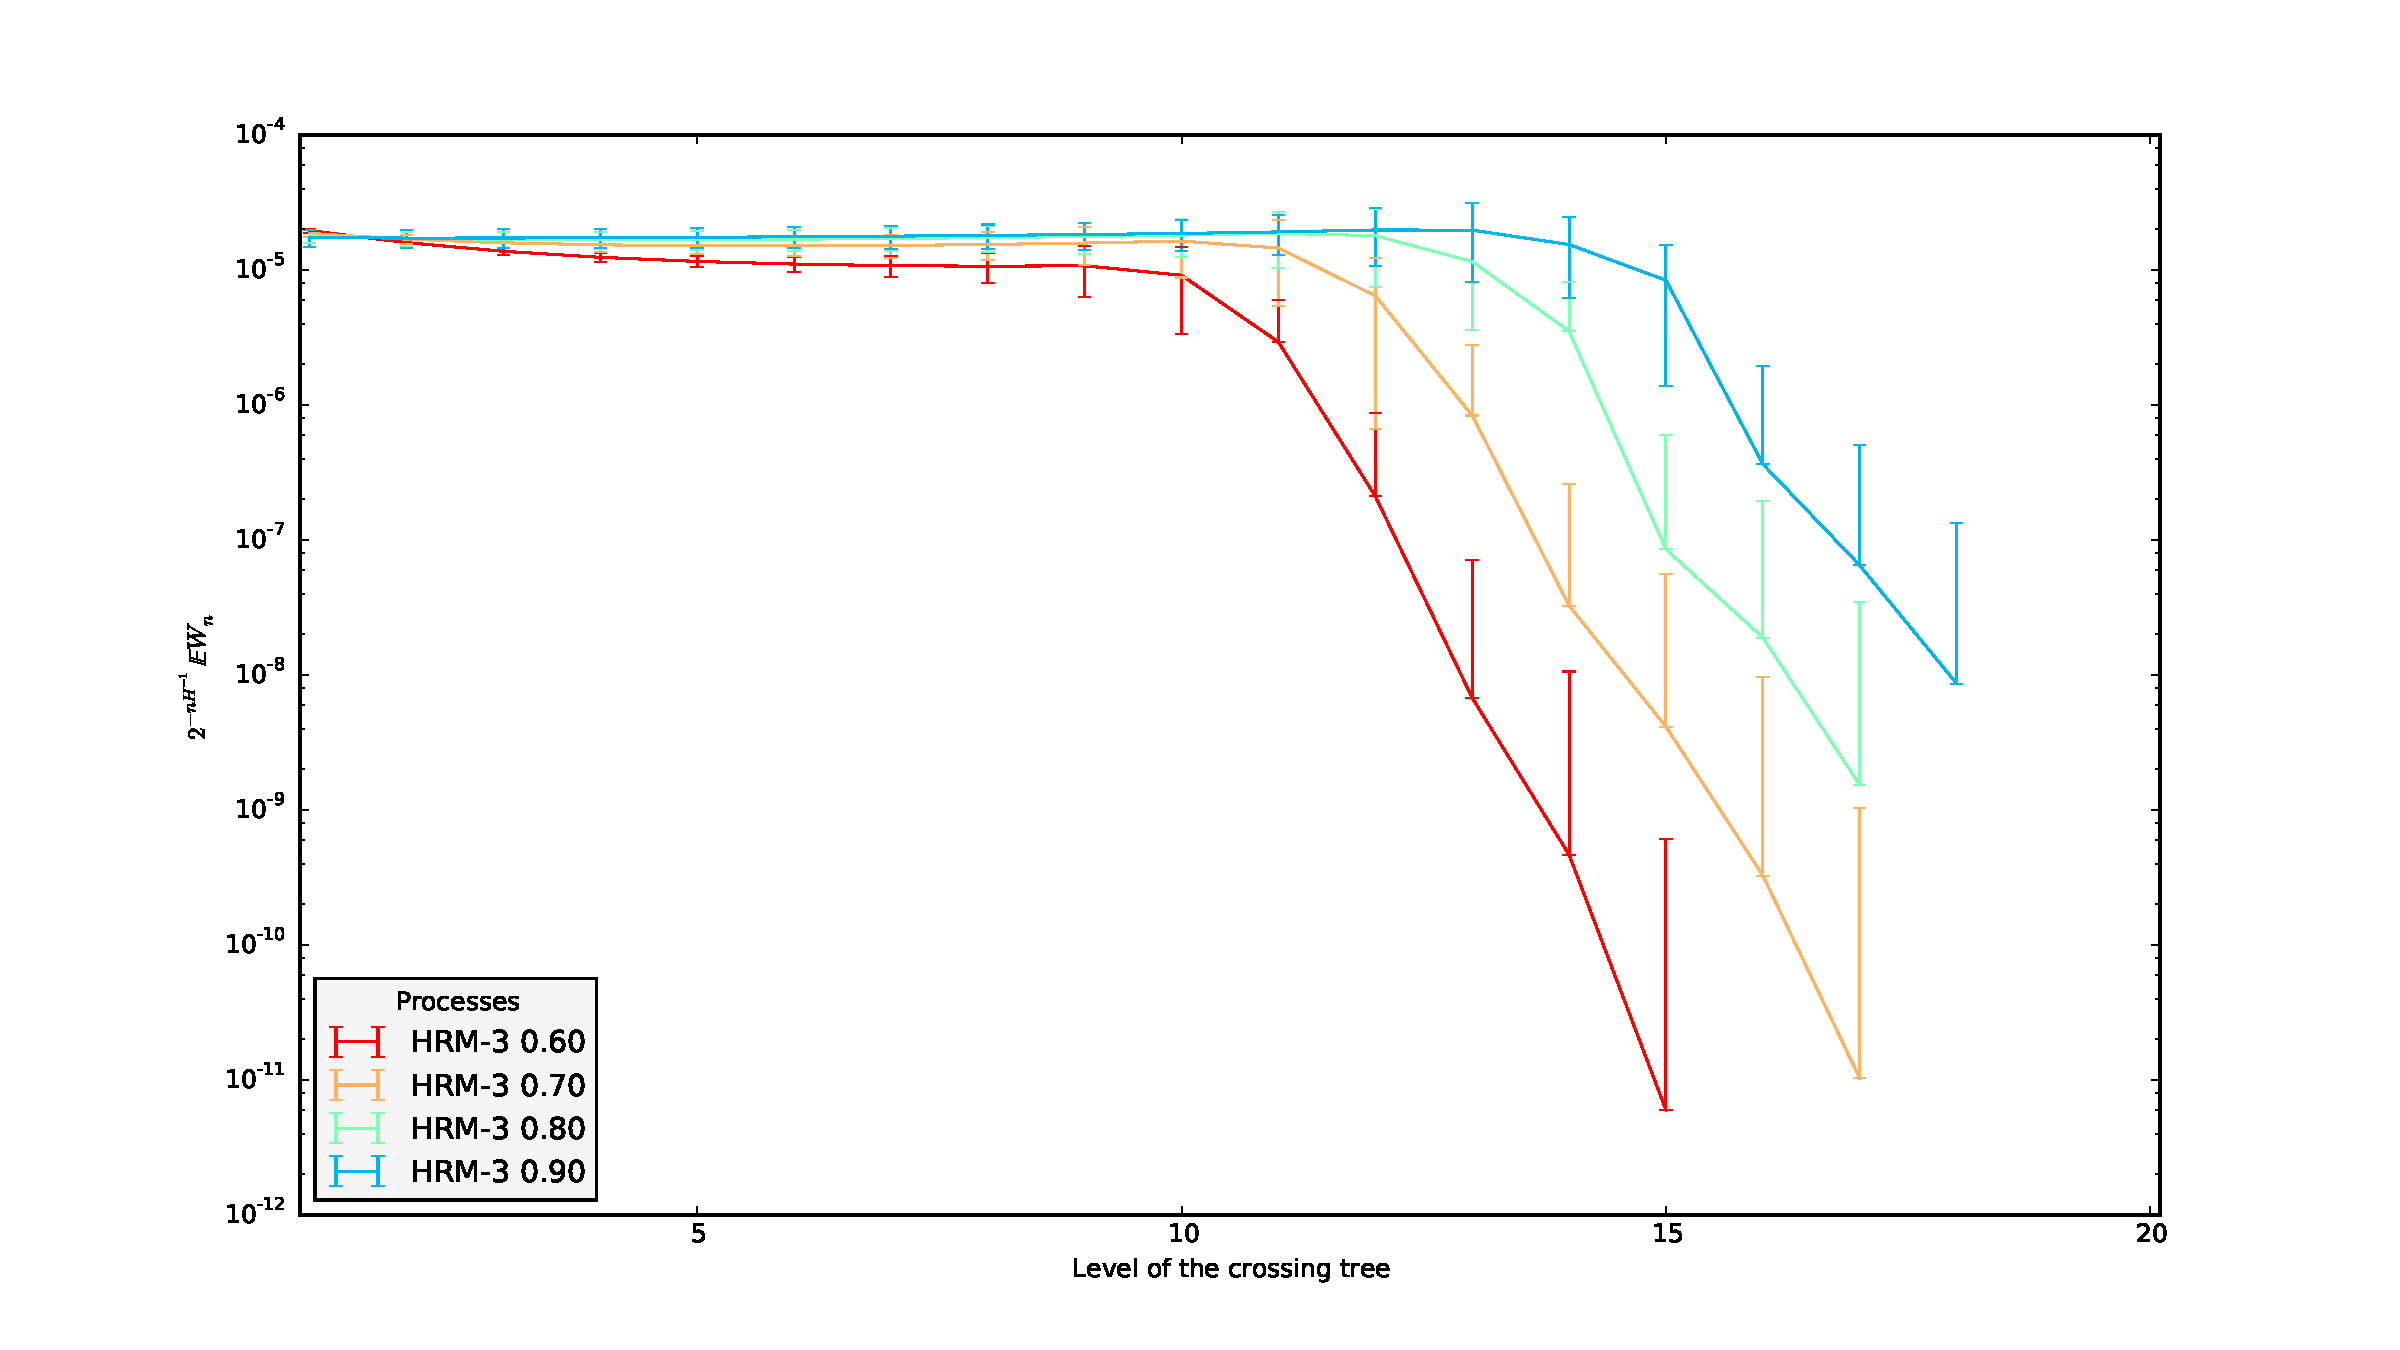
\includegraphics[width=6in]{images/fig_08_med_HRM-3_10000-17}
    \caption{The average crossing duration at each level of the crossing tree built
    for the Hermite processes of order $3$.}
\label{fig:hrm_3_durations}
\end{center}\end{figure}

\begin{figure}[htb]\begin{center}
    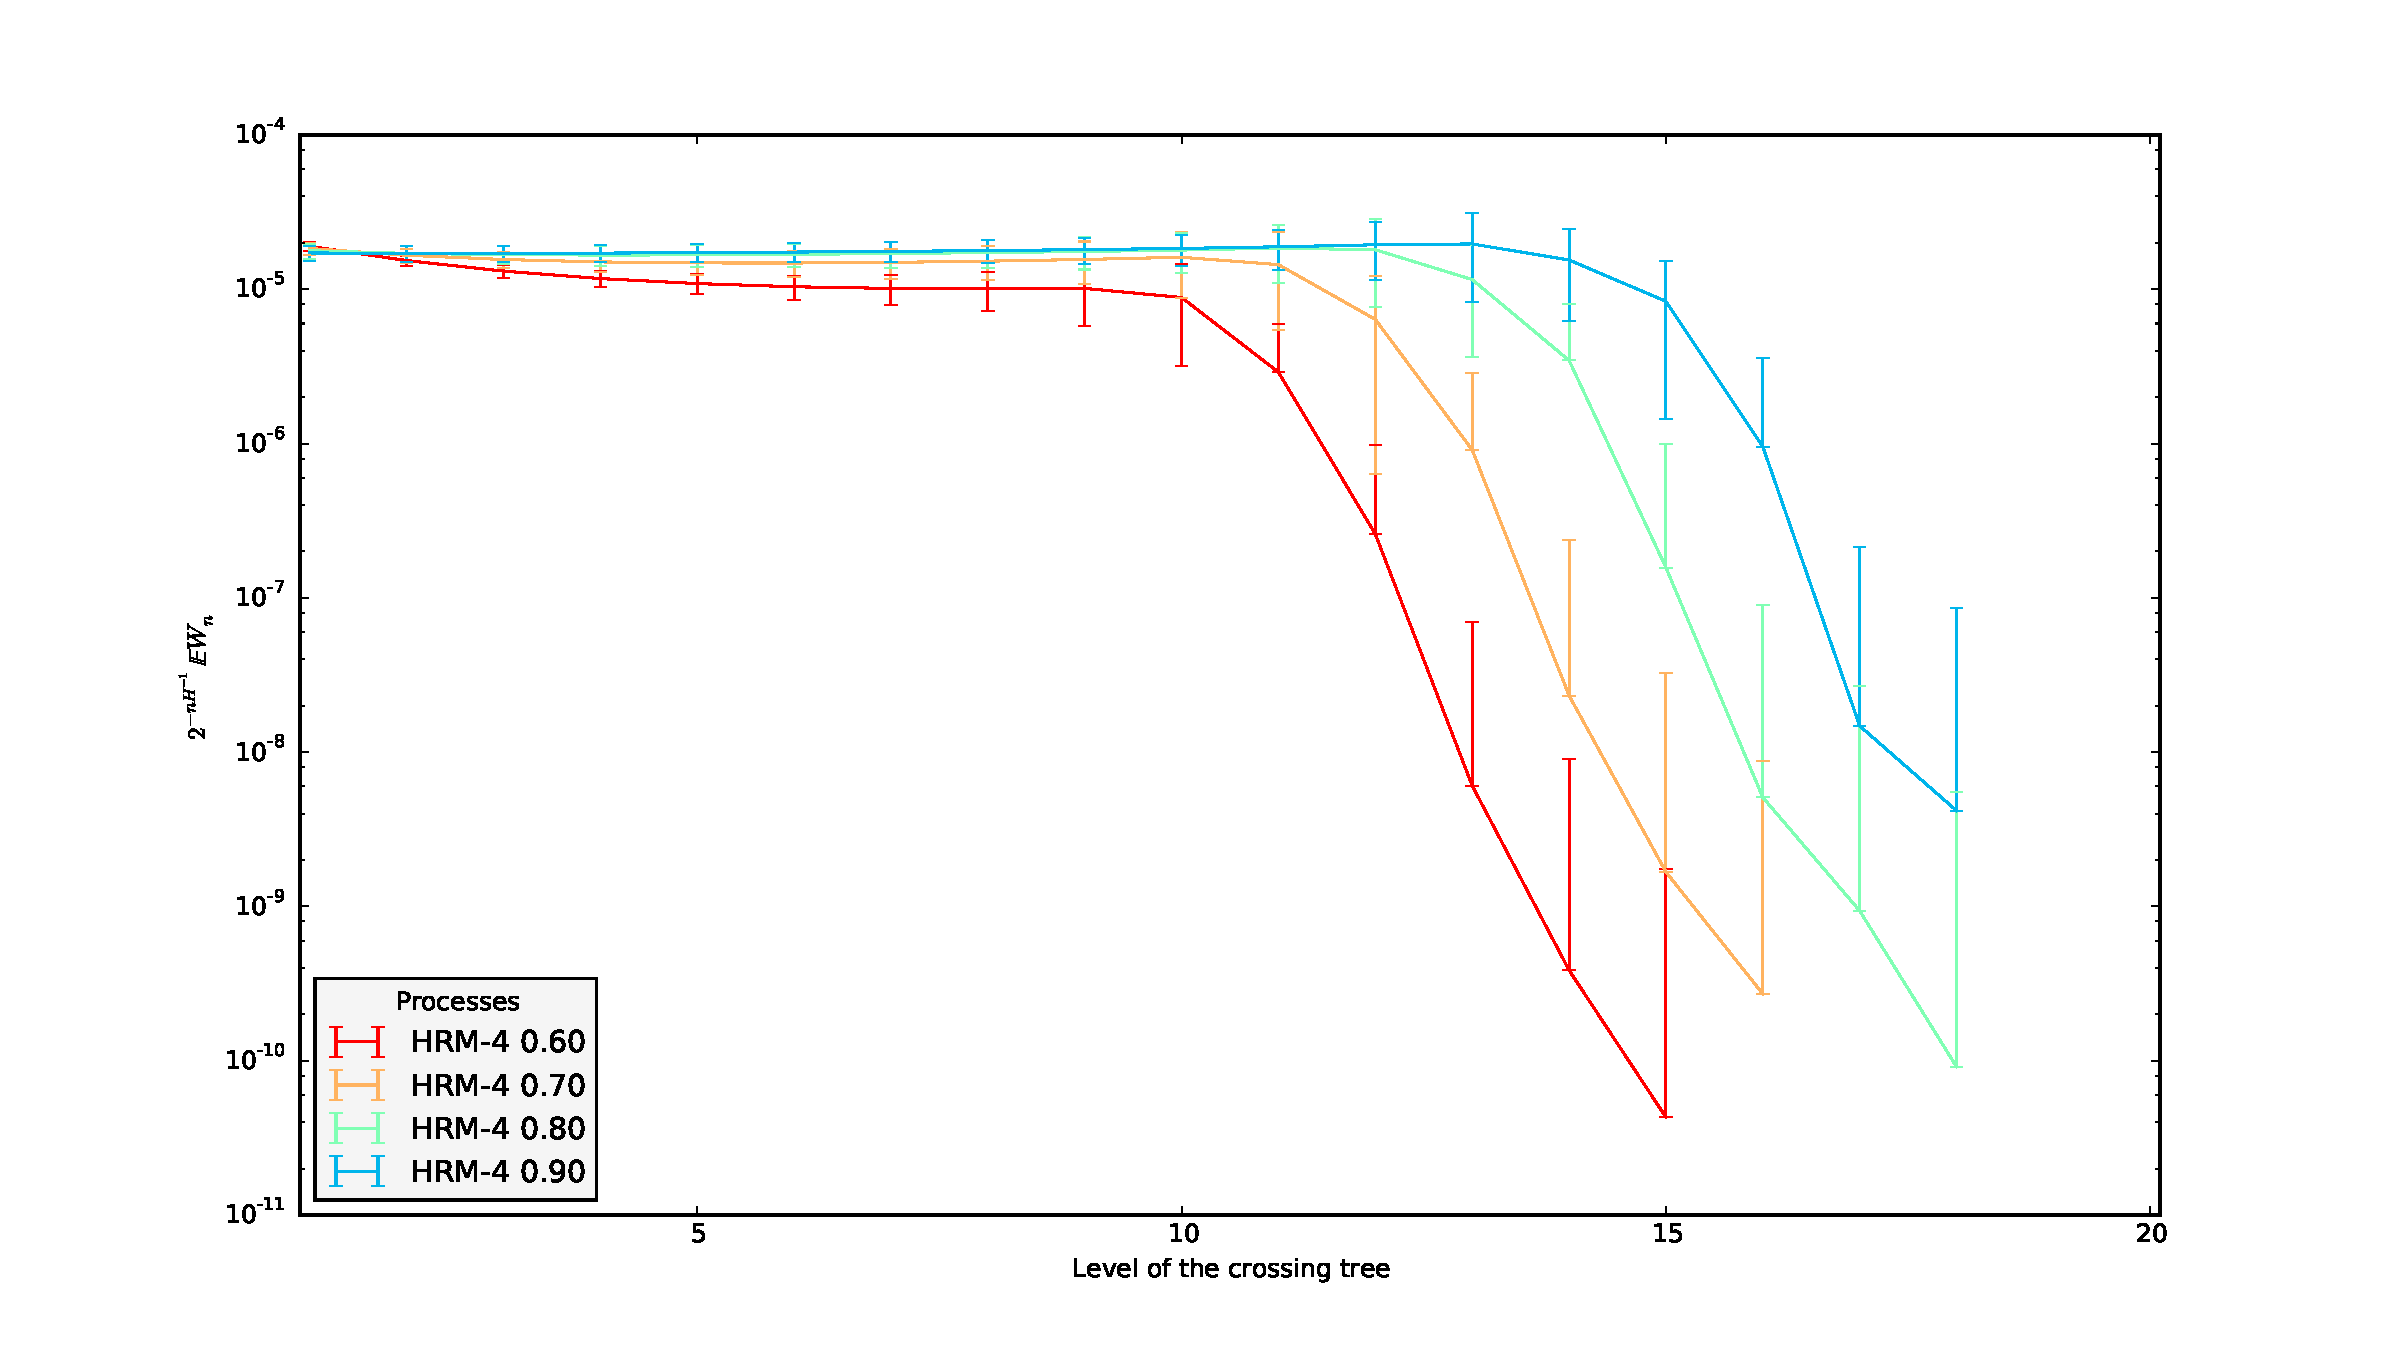
\includegraphics[width=6in]{images/fig_08_med_HRM-4_10000-17}
    \caption{The average crossing duration at each level of the crossing tree built
    for the Hermite processes of order $4$.}
\label{fig:hrm_4_durations}
\end{center}\end{figure}

\begin{figure}[htb]\begin{center}
    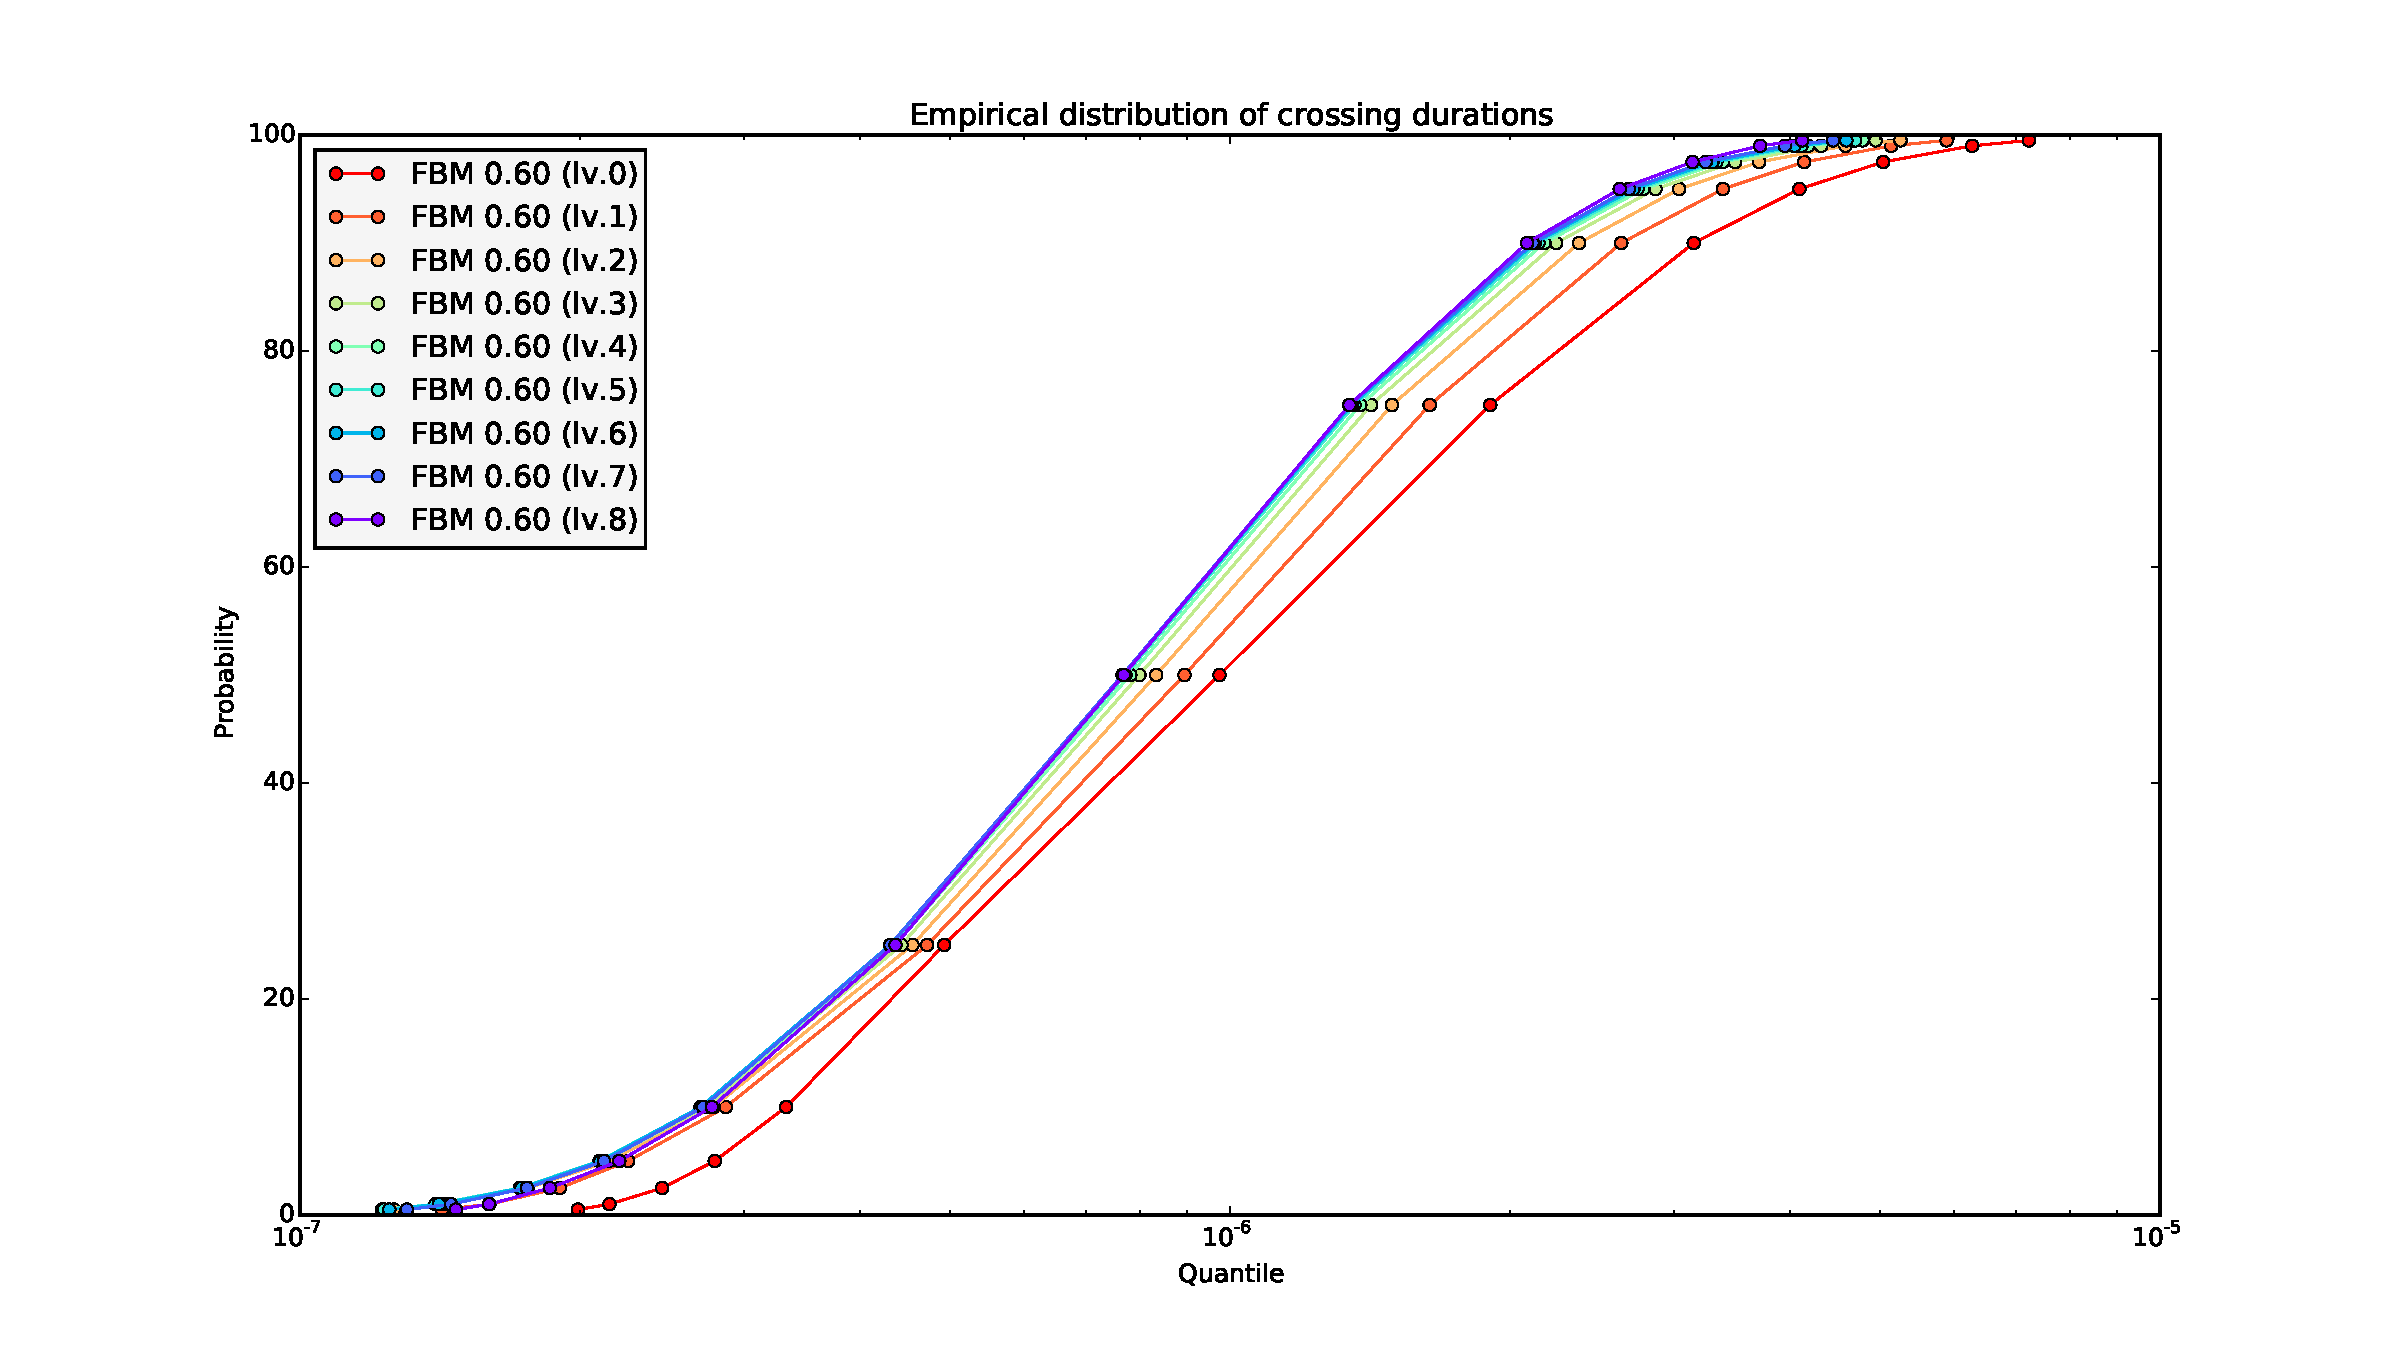
\includegraphics[width=6in]{images/fig_09_med_FBM_060}
    \caption{The empirical distribution of crossing durations at each level of the
    crossing tree built for the fractional Brownian motion ($2^{21}$ datapoints) with $H = 0.6$.
    Averaged across all Monte-Carlo realisations.}
\label{fig:fbm_quantiles_06}
\end{center}\end{figure}

\begin{figure}[htb]\begin{center}
    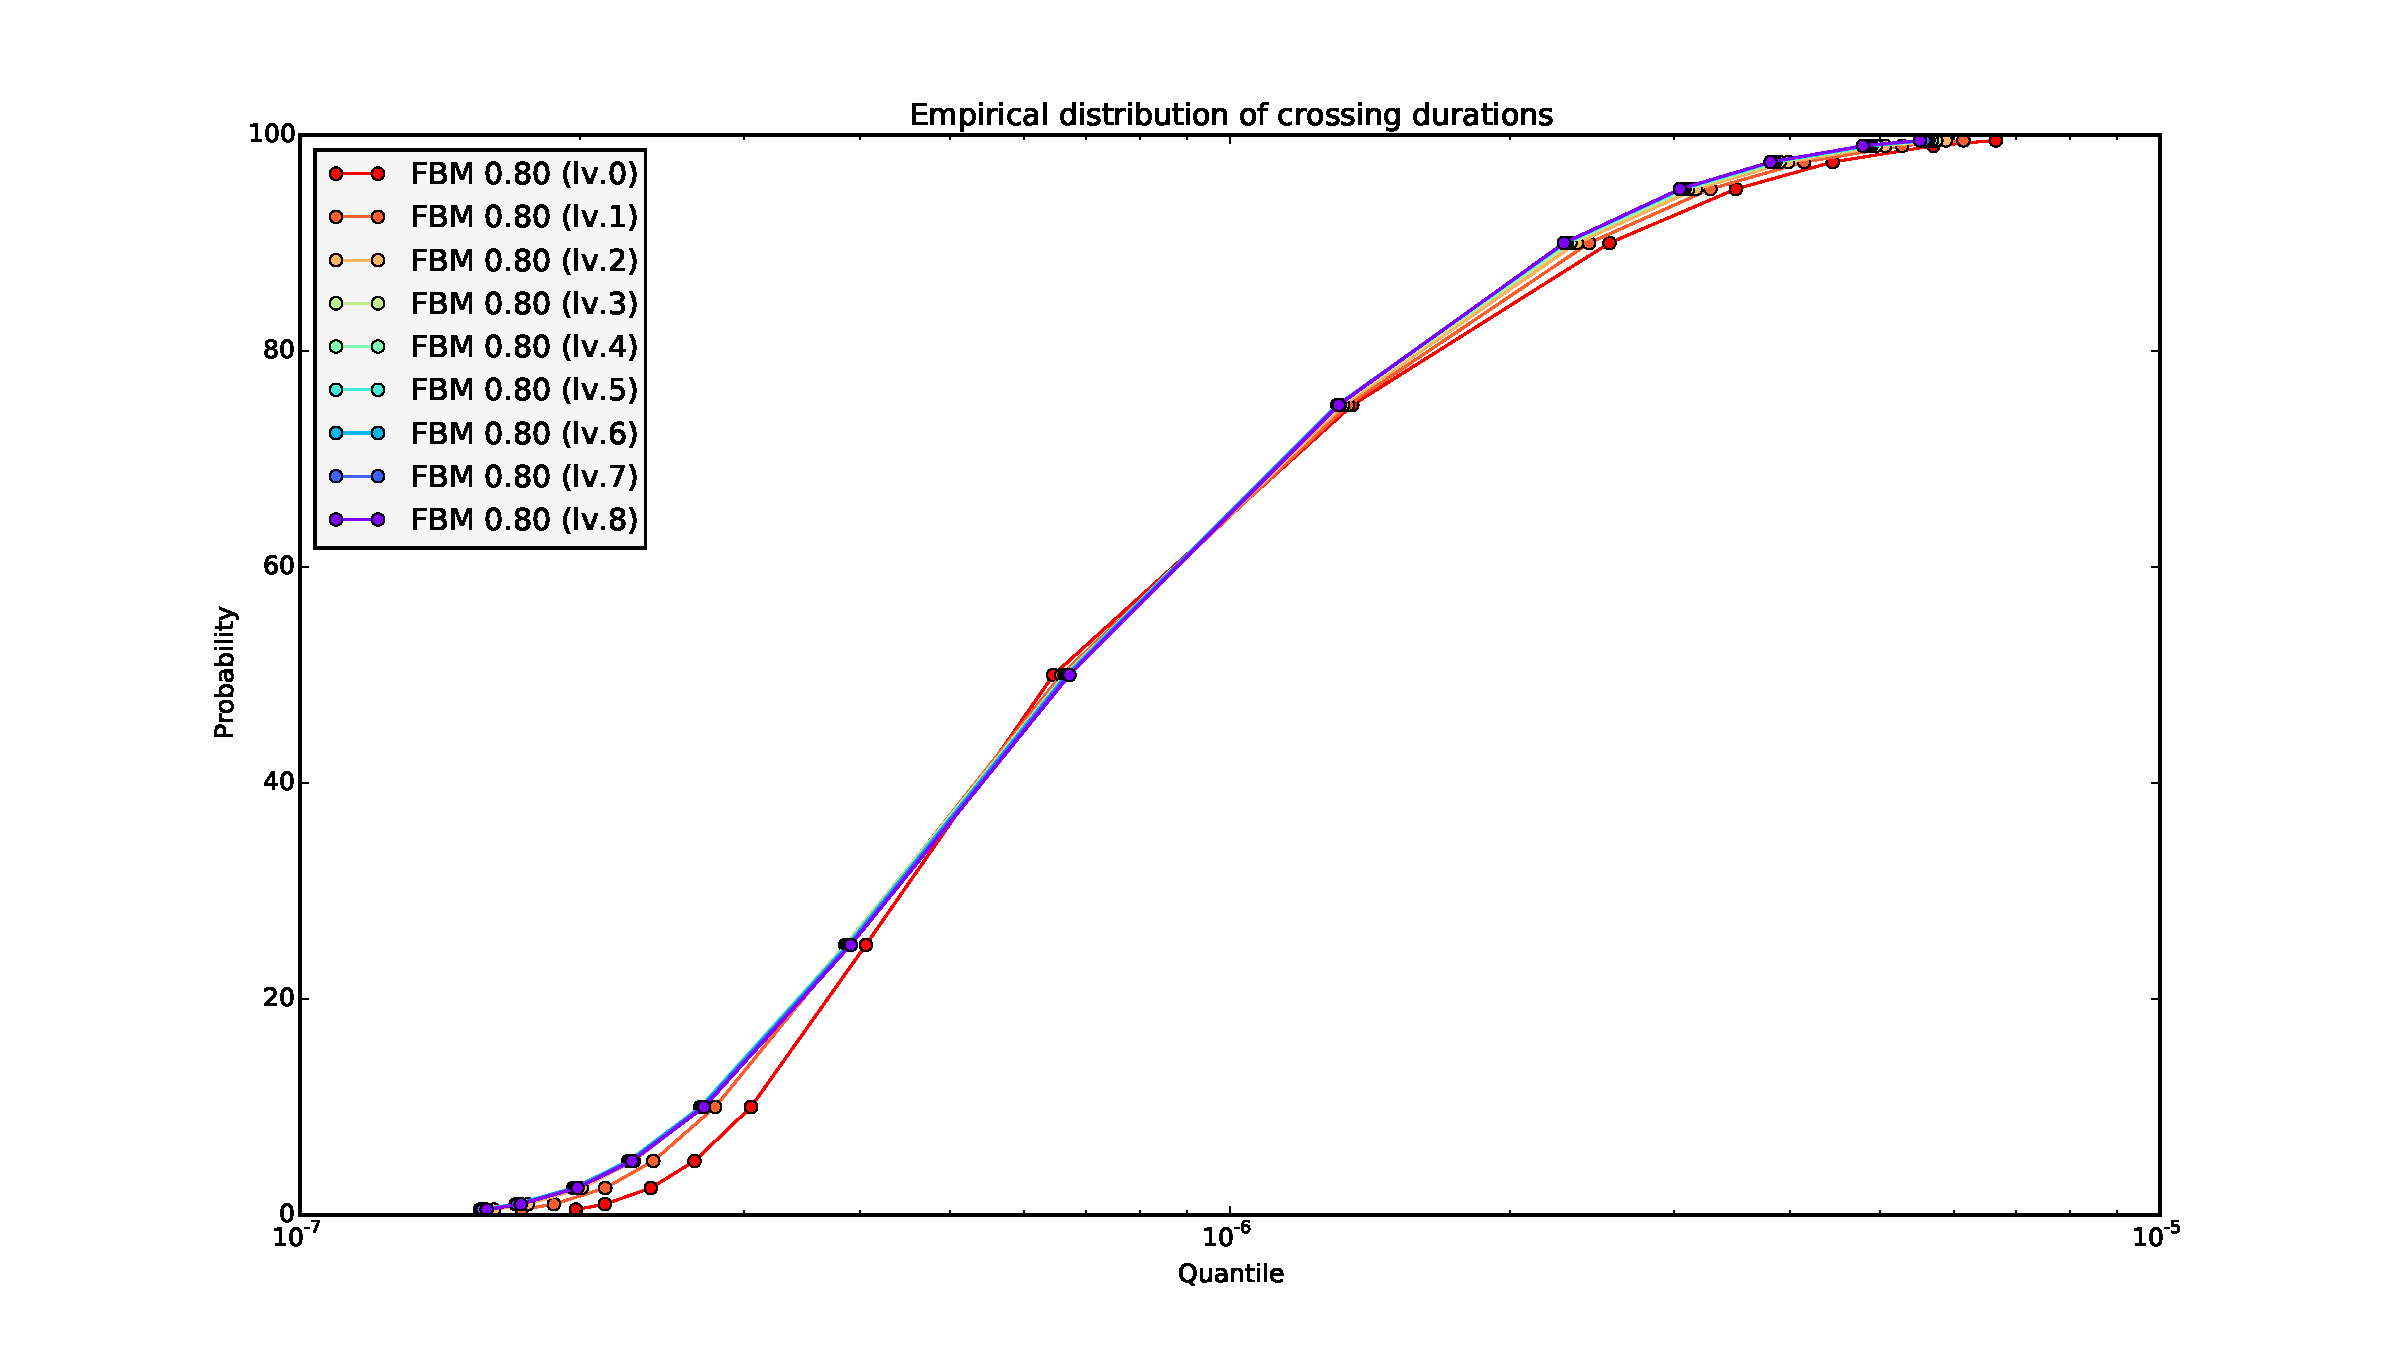
\includegraphics[width=6in]{images/fig_09_med_FBM_080}
    \caption{Similarly to figure~\ref{fig:fbm_quantiles_06} but for fBm with $H=0.8$.}
\label{fig:fbm_quantiles_08}
\end{center}\end{figure}

\begin{figure}[htb]\begin{center}
    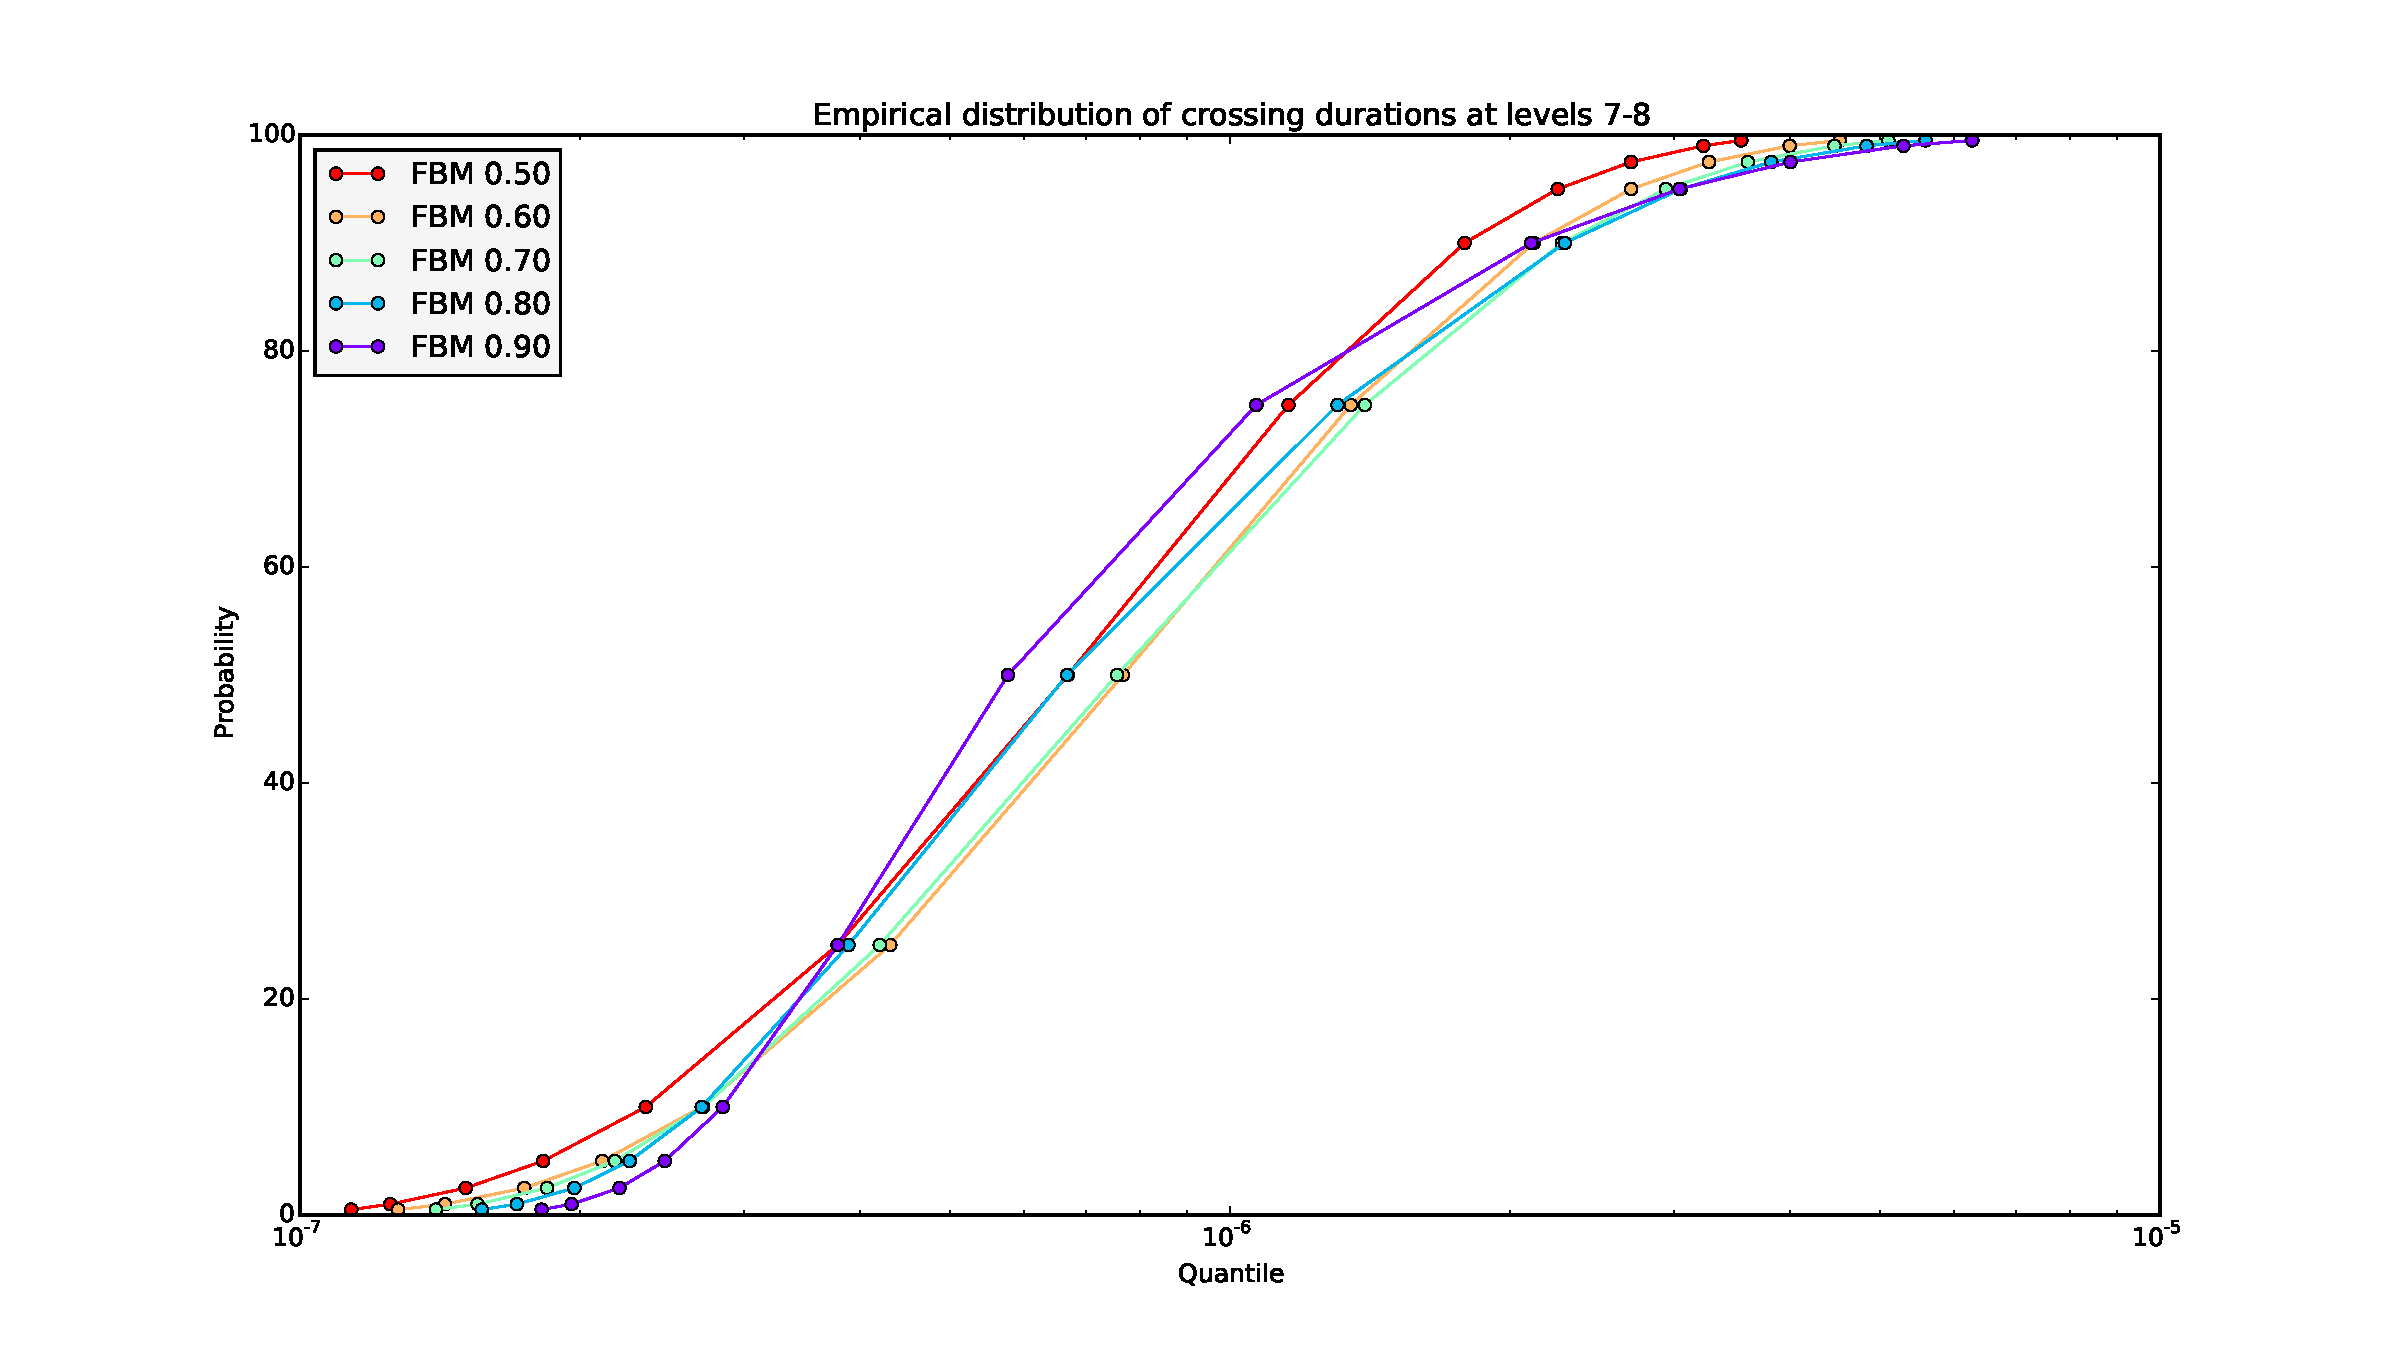
\includegraphics[width=6in]{images/fig_10_med_FBM}
    \caption{Empirical distributions of crossing durations estimated on levels 7-8
    for the fBm ($2^{21}$ datapoints). Averaged across all Monte-Carlo realisations.}
\label{fig:fbm_quantiles_durations}
\end{center}\end{figure}

% section results (end)


\section{Conclusion and further work} % (fold)
\label{sec:conlusion_and_further_work}

This preformed extensive Monte-Carlo simulation suggests, that the considered
classes of $H$-SSSI stochastic processes indeed shares common statistical properties
of the crossing tree. To findings are summarized below: \begin{enumerate}
	\item The crossing tree seems capable of correctly identifying the Hurst
	exponent of the studied series, provided correct tree levels are chosen to
	produce the estimate. The tree levels should not be too close to the leaves
	of the tree, for the sake of avoiding excessive bias due to linear interpolation,
	and be such that there is no statistical evidence to significant variations
	in the offspring distribution at each level;
	\item Processes seem to share similar shape of the empirical distribution of
	the crossing sizes (the number of offspring), though the hypothesized
	relationship between the offspring distribution and the Hurst exponent
	does not seem to hold exactly, (see figures \ref{fig:fbm_offspring_distribution}
	and \ref{fig:all_xing_probs});
	\item The conditional distributions of excursion within each crossing seems
	to agree with the hypothesised values of $2^{\frac{-1}{2H}}$.
	\item The collected empirical evidence seems to confirm similarity of the scaling
	properties of crossing durations across all studied processe.
\end{enumerate}
To summarize, the overall evidence is in favour of the conjecture, it is absolutely
necessary to address the issue of the upward bias in the empirical probabilities of
crossings of size higher than 2.

One of the way in which this study can be improved is the generation of samples paths
of Hermite stochastic processes. Another line of inquiry in the topic of crossing trees
if their application to machine learning and generalization to higher dimensions, which
would find application in image processing. The third possible extension is the utilization
of the crossing tree, or its modification, in the problem of early detection of structural
breaks in univariate or multivariate time series data.

% section conlusion_and_further_work (end)

\bibliographystyle{IEEEbib}
\bibliography{literature}

%% Supplementary material
\section*{Appendix} % (fold)
\label{sec:appendix}

\subsection*{Details on the practical procedure} % (fold)
\label{sub:details_on_the_practical_procedure}

% subsection* details_on_the_practical_procedure (end)

% section* appendix (end)

\end{document}
